\documentclass[a4paper, 11pt]{book}
\usepackage{anyfontsize}
\usepackage[CJKchecksingle, AutoFakeBold]{xeCJK}
\usepackage{CJKnumb}

\usepackage{setspace}
\onehalfspacing
\renewcommand{\arraystretch}{1}

\setlength{\parindent}{2em}

\usepackage[intlimits, leqno]{amsmath}
\usepackage{amssymb}
\usepackage[centercolon]{mathtools}
\usepackage{siunitx}

\usepackage{fontspec}
\usepackage{unicode-math}

\setmainfont[
    Extension=.otf,
    UprightFont=*-Regular,
    BoldFont=*-Bold,
    ItalicFont=*-Italic,
    BoldItalicFont=*-BoldItalic
]{STIXTwoText}

\setmathfont[
    Extension=.otf,
    BoldFont=*
]{STIXTwoMath-Regular}

\let\exerciseQuestion\Question
\AtBeginDocument{%
    \let\mathQuestion\Question
    \let\Question\exerciseQuestion
}

\setsansfont{TeX Gyre Heros}
\setmonofont{Courier New}

\usepackage{esint}

\DeclareSymbolFont{CMlargesymbols}{OMX}{cmex}{m}{n}
\let\sumop\relax\let\prodop\relax
\DeclareMathSymbol{\sumop}{\mathop}{CMlargesymbols}{"50}
\DeclareMathSymbol{\prodop}{\mathop}{CMlargesymbols}{"51}

\usepackage{euscript}

\newcommand{\bm}{\symbfit}
\newcommand{\smalltriangle}{\mathbin{\vcenter{\hbox{\scalebox{0.65}{$\triangle$}}}}}

\setCJKmainfont[
    ItalicFont=FZKai-Z03S
]{FZShuSong-Z01S}

\setCJKsansfont[
    BoldFont=* Medium,
    ItalicFont=FZKai-Z03S
]{Noto Sans CJK SC}

\setCJKmonofont[
    ItalicFont=FZKai-Z03S
]{FZShuSong-Z01S}

\setCJKfamilyfont{kai}{FZKai-Z03S}

\setCJKfamilyfont{song}[
    ItalicFont=FZKai-Z03S
]{FZShuSong-Z01S}

\setCJKfamilyfont{fangsong}[
    ItalicFont=FZKai-Z03S
]{FZFangSong-Z02S}

\setCJKfamilyfont{hei}{Noto Sans CJK SC Medium}
\setCJKfamilyfont{hei2}[
    BoldFont=* Bold
]{Noto Sans CJK SC}

\setCJKfamilyfont{black}[
    BoldFont=* Black
]{Noto Sans CJK SC}

\setCJKfamilyfont{sectionfont}[
    BoldFont=* Black
]{Noto Sans CJK SC}

\setCJKfamilyfont{pffont}[
    BoldFont=* Medium
]{Noto Sans CJK SC}

\setCJKfamilyfont{emfont}[
    BoldFont=* Medium
]{Noto Sans CJK SC}

\defaultfontfeatures{Ligatures=TeX} 
\XeTeXlinebreaklocale "zh"
\XeTeXlinebreakskip=0pt plus 1pt minus 0.1pt

\newcommand\kaishu{\CJKfamily{kai}}
\newcommand\songti{\CJKfamily{song}}
\newcommand\heiti{\CJKfamily{hei}}
\newcommand\thmheiti{\CJKfamily{hei2}}
\newcommand\fangsong{\CJKfamily{fangsong}}
\renewcommand{\em}{\bfseries\CJKfamily{emfont}}


\usepackage[unicode, colorlinks, bookmarksnumbered]{hyperref}
\hypersetup{
	linkcolor=blue,
	citecolor=red,
	urlcolor=teal,
	pdfauthor={王畅},
	pdftitle={ICS 问题求解(2021 秋)}
}

\usepackage[iso, english]{isodate}
\usepackage{geometry}
\geometry{
	paper=a4paper,
	top=3cm,
	inner=2.54cm,
	outer=2.54cm,
	bottom=3cm,
	headheight=6ex,
	headsep=6ex,
}

\usepackage[svgnames, dvipsnames, table]{xcolor}

\usepackage{paralist}
\usepackage{commands}
\usepackage[font=small, labelfont=bf]{caption}
\usepackage{graphicx}
\usepackage{float}
\usepackage{longtable}
\usepackage{multirow}
\usepackage{tikz}
\usetikzlibrary{shapes.symbols, backgrounds, matrix, calc, arrows, math, arrows.meta, shapes.gates.logic.US, shapes.gates.logic.IEC, decorations.pathreplacing}
\usepackage{minted}
\renewcommand\fcolorbox[4][]{\textcolor[rgb]{0.63,0.63,0.00}{\strut#4}}
\renewcommand{\theFancyVerbLine}{\texttt{\scriptsize{\arabic{FancyVerbLine}}}}
\tikzset{hassenode/.style={circle, draw=black, fill=white, inner sep=1pt, minimum size=5pt}}

\newcommand\MemoryLayout[2]{
	\begin{tikzpicture}[scale=0.3]
		% \draw[thick] (0,0) -- ++(0,3) node[above] {$0$};
		\foreach \pt/\col/\lab [remember=\pt as \tp (initially 0)] in {#1} {
			\pgfmathparse{\pt-1}
			\foreach \a in {\tp, ..., \pgfmathresult} {
				\draw[fill=\col] (-\a,0) rectangle ++(-1,2);
			}
			% \draw[thick] (-\pt,0) -- ++(0,3) node[above] {$\pt$};
			\if\lab\relax\relax\else
				\draw[thick, decorate, decoration={brace, amplitude=4mm}] (-\tp,-0.2) -- node[below=4mm]{\lab} (-\pt,-0.2);
			\fi
    	}
		#2
  	\end{tikzpicture}
}

\numberwithin{equation}{chapter}
\renewcommand{\theequation}{\thechapter.\arabic{equation}}

\usepackage{ulem}
\normalem

\usepackage{datetime}

\usepackage{xstring}
\usepackage{wasysym}
\usepackage{fancyhdr}
\newcommand\sectionname{\arabic{chapter}.\arabic{section}}
\pagestyle{fancy}
\renewcommand{\chaptermark}[1]{\markboth{
	\CJKnumber{\thechapter}\quad #1
}{}}
\renewcommand{\sectionmark}[1]{\markright{\arabic{chapter} \quad #1}}
\fancyhf{}
\fancyhead[EC]{\CJKfamily{hei2}\footnotesize{\leftmark}\vspace{1mm}}
\fancyhead[OC]{\CJKfamily{hei2}\footnotesize{\leftmark}\vspace{1mm}}
\fancyhead[LE, RO]{{\footnotesize \thepage}\vspace{1mm}}
\fancyhead[RE, LO]{}
\renewcommand{\headrulewidth}{0.5pt}
\renewcommand{\footrulewidth}{0pt}
\addtolength{\headheight}{0.5pt}
\renewcommand{\headrulewidth}{0pt}
\renewcommand{\footrulewidth}{0pt}
\addtolength{\headheight}{0.5pt}

\usepackage[many]{tcolorbox}

\newtcolorbox{summary}{
	breakable,
	enhanced,
	width=\textwidth,
	colback=white, colbacktitle=white,
	colframe=gray!50, boxrule=0.2mm,
	coltitle=black,
	fonttitle=\bfseries\sffamily,
	attach boxed title to top left={yshift=-\tcboxedtitleheight/2, xshift=\tcboxedtitlewidth/4},
	boxed title style={boxrule=0pt, colframe=white},
	after skip=1cm,
	top=3mm,
	bottom=3mm,
	title={要点}
}

\usepackage[calcwidth, explicit, nobottomtitles, newparttoc, indentafter]{titlesec}
\usepackage{titletoc}
\usepackage[titles]{tocloft}
\cftsetpnumwidth{1.75em}
\providecommand{\dmchapterttl}[1]{\IfSubStr{ABCDEFGHIJKLMNOPQRSTUVWXYZ}{#1}{附录 #1	}{\CJKnumber{#1}}}

\newlength{\BoxTtlwidth}

\newcommand{\MakeChapBox}[2]{%
	\settowidth{\BoxTtlwidth}{\dmchapterttl{#1}}
	\begin{tcolorbox}[
		enhanced jigsaw,
		skin=bicolor,
		frame engine=path,
		sharp corners=all,
		width=0.9\textwidth,
		top=4mm, bottom=4mm,
		sidebyside,
		frame hidden,
		boxrule=0mm,
		lefthand width=\BoxTtlwidth,
		colupper=white,
		colback=gray!80,
		colbacklower=gray!10,
		sidebyside align=center,
		halign=center]
		\dmchapterttl{#1}
		\tcblower
		#2
	\end{tcolorbox}%
}

\newcommand{\MakeChapBoxSingle}[1]{%
	\begin{tcolorbox}[
		enhanced,
		width=0.7\textwidth,
		sharp corners=all,
		top=4mm, bottom=4mm,
		frame hidden,
		boxrule=0mm,
		colback=gray!10,
		halign=center]
		#1
	\end{tcolorbox}
}

\newtcbox{\MakeSectBox}{
	enhanced,
	arc=0pt, outer arc=0pt,
	before skip=0pt, after skip=0.4em, left skip=0pt, right skip=0pt,
	top=0pt, left=0pt, right=0pt, bottom=1.5mm,
	sharp corners=all,
	valign=bottom,
	colback=white,
	colframe=white,
	boxsep=0pt, leftrule=0pt, rightrule=0pt, toprule=0pt, bottomrule=0pt,
	overlay={ \draw[line width=1pt] (interior.south west) -- (interior.south east); }
}

\newcommand*\chapterlabel{}
\titleformat{\chapter}
  	{\gdef\chapterlabel{}\sffamily\CJKfamily{black}\bfseries\Huge}
  	{\gdef\chapterlabel{\thechapter\ }}{0pt}
  	{\begin{tikzpicture}[remember picture, overlay]
		\node[yshift=-3cm] at (current page.north west)
	  		{\begin{tikzpicture}[remember picture, overlay]
				\draw[fill=titlepagecolor!20] (0,0) rectangle (\paperwidth, 3cm);
				\node[anchor=east, xshift=0.9\paperwidth, rectangle,  rounded corners=20pt, inner sep=11pt, fill=titlepagecolor] {\color{white} {\fontsize{48}{60}\selectfont\chapterlabel}#1};
			\end{tikzpicture}};
   	\end{tikzpicture}
}
\titlespacing*{name=\chapter, numberless}
	{1pc}{*4}{1em}

\titleformat{name=\section}
	{\filleft\normalfont\sffamily\bfseries\CJKfamily{sectionfont}}
	{}
	{0mm}
	{ \settowidth{\BoxTtlwidth}{\Huge \thesection \hspace{0.7em} \Large #1}
		\ifdim \BoxTtlwidth < \textwidth
			\MakeSectBox{\Huge \thesection \hspace{0.7em} \Large #1}\vskip-18pt%
		\else
			\Huge \underline{\thesection} \hspace{0.7em} \Large #1%
		\fi%
	}
	[]

\titleformat{name=\section, numberless}
	{\filleft\normalfont\sffamily\bfseries\CJKfamily{sectionfont}}
	{}
	{0mm}
	{ \settowidth{\BoxTtlwidth}{\Large #1}
		\ifdim \BoxTtlwidth < \textwidth
			\MakeSectBox{\Large #1}\vskip-18pt%
		\else
			\Large #1
		\fi
	}
	[]
	
\titlespacing*{name=\section}
	{1pc}{*1.3}{*1}

\usepackage{zhnumber}
\usepackage[answerdelayed, lastexercise]{exercise}
\renewcommand{\ExerciseListName}{}
\renewcommand{\AnswerListName}{}
\renewcommand{\ExerciseHeaderNB}{\theExercise}
\renewcommand{\QuestionNB}{(\arabic{Question})}
\renewcommand{\ExerciseHeaderOrigin}{\ ({\kaishu\ExerciseOrigin})}
\renewcommand{\ExerciseListHeader}{\ExerciseHeaderDifficulty\textbf{\ExerciseHeaderNB}\textbf{.}\ExerciseHeaderOrigin\enspace}
\renewcommand{\AnswerListHeader}{\textbf{\ExerciseHeaderNB.}\enspace}
\renewcounter{Exercise}[chapter]
\renewcommand{\AtBeginAnswer}{\vspace{-1\baselineskip}}
\newcommand{\pro}{\Exercise}
\newcommand{\qn}{\Question}
\newcommand{\subqn}{\subQuestion}
\newcommand{\sol}{\Answer}
\setlength{\subQuestionBefore}{.25em}

\makeatletter
\renewcommand{\@@@ExeCmd}{%
	\ifnum\@QuestionLevel=0
		\advance \@QuestionLevel by 1
		\begin{list}{\@getExerciseInfo\ExerciseListHeader}%
		{\partopsep \Exepartopsep \labelsep \Exelabelsep \itemsep \Exesep \listparindent 2em%
		\parsep \Exeparsep \topsep \Exetopsep \labelwidth \Exelabelwidth%
		\leftmargin \Exeleftmargin \rightmargin \Exerightmargin}
	\else
		\termineliste{1}\@EndExeBox
	\fi
	\@selectExercise
	\global\@Answerfalse\@BeginExeBox\refstepExecounter%
	\addcontentsline{\ext@exercise}{\toc@exercise}{\ExerciseName\
	\theExercise\ \expandafter{\itshape \ExerciseTitle}\hspace{.66em}}
	\item\ignorespaces\AtBeginExercise
}
\makeatother

\newcounter{soleq}
\counterwithin{soleq}{chapter}
\newenvironment{soleq}{\refstepcounter{soleq}\equation}{\tag{S-\thesoleq}\endequation}

\makeatletter
\newenvironment{problems}{%
	\begin{ExerciseList}
		\global\setbox\temp@Answerbox%
		\vbox{\unvbox\all@Answerbox\vspace{1cm}\section*{参考答案\zhnum{chapter}}\unvbox\@Exercisebox\vskip\z@}%
		\global\setbox\all@Answerbox\copy\temp@Answerbox
		}{
	\end{ExerciseList}
}

\newenvironment{choices}{\begin{compactenum}[\quad\ \,A.{\ \ \ }]}{\end{compactenum}}

\newenvironment{hint}{%
	\ifvmode
		\ignorespaces
	\else
		\quad
	\fi
	\begin{tikzpicture}[baseline=(H.base), every node/.style={signal, draw, very thin, signal to=east, signal from=nowhere, signal pointer angle=120, inner sep=2pt}]
		\node[anchor=mid west] (H) at (0,0) {\heiti\footnotesize 提示};
	\end{tikzpicture}
}{}

\g@addto@macro\frontmatter{\setcounter{tocdepth}{1}
	\setcounter{page}{1}
	\thispagestyle{empty}
	\addtocontents{toc}{\protect\thispagestyle{empty}}
	
	\renewcommand{\contentsname}{目录}
	\tableofcontents
}

\renewcommand{\figurename}{图}
\renewcommand{\tablename}{表}

\renewcommand{\listfigurename}{图片索引}
\renewcommand{\listtablename}{表格索引}

\pretocmd{\listoffigures}{%
	\cleardoublepage
	\phantomsection
	\addcontentsline{toc}{chapter}{\listfigurename}
}{}{}
\pretocmd{\listoftables}{%
	\cleardoublepage
	\phantomsection
	\addcontentsline{toc}{chapter}{\listtablename}
}{}{}

\usepackage[thmmarks, amsmath, hyperref]{ntheorem}
\theoremstyle{change}
\theorembodyfont{\fangsong}
\theoremheaderfont{\sffamily\bfseries\thmheiti}
\theoremseparator{\ }
\setlength{\theorempreskipamount}{2mm}
\setlength{\theorempostskipamount}{2mm}

\newtheorem{theorem}{定理}[chapter]

\theorembodyfont{\songti}
\newtheorem{problem}[theorem]{例题}
\newtheorem{example}[theorem]{例}

\theorembodyfont{}
\theoremstyle{nonumberplain}
\theoremheaderfont{\sffamily\bfseries\CJKfamily{pffont}}
\theoremseparator{\enspace}
\theoremsymbol{}
\newtheorem{solution}{解}

\numberwithin{equation}{section}
\renewcommand{\theequation}{\thesection.\arabic{equation}}
\allowdisplaybreaks

\newcommand{\proy}[1]{\pro[origin={#1}]}
\newcommand*\circled[1]{\tikz[baseline=(char.base)]{\node[shape=circle, draw, inner sep=0.5pt] (char) {#1};}}

\usepackage{epigraph}

\renewcommand\epigraphflush{flushright}
\renewcommand\epigraphsize{\normalsize}
\setlength\epigraphwidth{0.7\textwidth}

\definecolor{titlepagecolor}{cmyk}{1, 0.6, 0, 0.4}

\newcommand\titlepagedecoration{%
	\begin{tikzpicture}[remember picture,overlay,shorten >= -10pt]
		\coordinate (aux1) at ([yshift=-15pt] current page.north east);
		\coordinate (aux2) at ([yshift=-410pt] current page.north east);
		\coordinate (aux3) at ([xshift=-4.5cm] current page.north east);
		\coordinate (aux4) at ([yshift=-150pt] current page.north east);

		\begin{scope}[titlepagecolor!40, line width=12pt, rounded corners=12pt]
			\draw (aux1) -- coordinate (a) ++(225:5) -- ++(-45:5.1) coordinate (b);
			\draw[shorten <= -10pt] (aux3) -- (a) -- (aux1);
			\draw[opacity=0.6,titlepagecolor,shorten <= -10pt] (b) -- ++(225:2.2) -- ++(-45:2.2);
		\end{scope}
		
		\draw[titlepagecolor, line width=8pt, rounded corners=8pt, shorten <= -10pt] (aux4) -- ++(225:0.8) -- ++(-45:0.8);
		
		\begin{scope}[titlepagecolor!70, line width=6pt, rounded corners=8pt]
			\draw[shorten <= -10pt] (aux2) -- ++(225:3) coordinate[pos=0.45] (c) -- ++(-45:3.1);
			\draw (aux2) -- (c) -- ++(135:2.5) -- ++(45:2.5) -- ++(-45:2.5) coordinate[pos=0.3] (d);   
			\draw (d) -- +(45:1);
		\end{scope}
	\end{tikzpicture}%
}

\begin{document}
	\begin{titlepage}
		\noindent
		{\fontsize{40}{40} \selectfont \bfseries \sffamily \CJKfamily{sectionfont} ICS 问题求解} \par
		\vspace{1cm}
		\epigraph{\LARGE PKU 04832363:计算机系统导论讨论班}{\Large 2021 年秋}
		\null\vfill
		\begin{center} \href{https://www.pku.edu.cn/}{
\includegraphics[height=60pt]{logo.eps}} \end{center}
		\titlepagedecoration
	\end{titlepage}
	\newpage
	\thispagestyle{empty}
	\begin{center}
		\LARGE 编译于 {\today} \currenttime
	\end{center}
	\vfill
	\begin{flushleft}
		\large \textbf{汇编:} 王畅 \\
    	\textbf{勘误:} 请写信到 \href{mailto:wchang@pku.edu.cn}{\texttt{wchang@pku.edu.cn}} \\
		\vspace{\baselineskip}
		\textbf{说明:}以下内容是 2021 年秋计算机系统导论讨论班(04832363,班号 16)使用的材料。主要的练习题均来源于往年计算机系统导论课程,编者仅做了汇编和微小的改动。考题只选择了 2018 年及之前的内容,不选用更新的题目是因为 2019 年和 2020 年的试卷将留给大家复习备考时整套使用。有关 Lab 的指导则为编者自行组织。后面附有部分题目的分析和答案,“部分”选择的要旨是对较难的题目作详细解释;对于往年题我们只给出较难的题或者无答案题的分析。
	\end{flushleft}

	\frontmatter

	\mainmatter
	\chapter{位级表示}\thispagestyle{empty}
    \begin{summary}
        \begin{compactitem}
            \item 知道整数、浮点数在系统的存储方式(字节序)。
            \item 熟练掌握整数、浮点数的位级表示规则,快速完成其同十进制数的相互转换。
            \item 理解整数、浮点数规范中的各类特殊数的计算方法及其性质。
            \item 运用浮点数舍入的规则进行运算,知道类型转换的基本规则,能针对整数、浮点数的一些常见“反常情况”进行判断。
        \end{compactitem}
    \end{summary}

    \begin{problems}
        \pro 在 x86-64 机器上,定义 \texttt{unsigned int A = 0x123456}。请画出 \texttt{A} 在内存中的存储方式:
        \begin{table}[H]
            \centering
            \begin{tabular}{|c|c|c|c|c|c|c|c|}
                \hline
                ... & 低地址 & \multicolumn{4}{c|}{\texttt{A}} & 高地址 & ... \\ \hline
                \multicolumn{2}{|c|}{...} & {\qquad \qquad} & {\qquad \qquad} & {\qquad \qquad} & {\qquad \qquad} & \multicolumn{2}{c|}{...} \\ \hline
            \end{tabular}
        \end{table}
        定义 \texttt{unsigned short B[2] = \{0x1234, 0x5678\}}。请画出 \texttt{B} 在内存中的存储方式:
        \begin{table}[H]
            \centering
            \begin{tabular}{|c|c|c|c|c|c|c|c|}
                \hline
                ... & 低地址 & \multicolumn{4}{c|}{\texttt{B}} & 高地址 & ... \\ \hline
                \multicolumn{2}{|c|}{...} & {\qquad \qquad} & {\qquad \qquad} & {\qquad \qquad} & {\qquad \qquad} & \multicolumn{2}{c|}{...} \\ \hline
            \end{tabular}
        \end{table}
        \sol 根据小端法可知分别为 \verb|0x56 0x34 0x12 0x00|、\verb|0x34 0x12 0x78 0x56|。
        \pro 在 x86-64 机器上,有下列 C 代码:
        \begin{minted}[frame=single, fontsize=\small, linenos]{c}
    int main() {
        unsigned int A = 0x11112222;
        unsigned int B = 0x33336666;
        void *x = (void *)&A;
        void *y = 2 + (void *)&B;
        unsigned short P = *(unsigned short *)x;
        unsigned short Q = *(unsigned short *)y;
        printf("0x%04x", P + Q);
        return 0;
    }
        \end{minted}
        运行该代码,结果是什么?
        \sol 根据小端法,\verb|A| 在内存中从高地址到低地址分别是 \verb|11 11 22 22|,得到 \verb|P = 0x2222|,同理 \verb|Q = 0x3333|,结果为 \verb|0x5555|。
        \pro 在 x86-64 机器上,有下列 C 代码:
        \begin{minted}[frame=single, fontsize=\small, linenos]{c}
    int main() {
        char A[12] = "11224455";
        char B[12] = "11445577";
        void *x = (void *)&A;
        void *y = 2 + (void *)&B;
        unsigned short P = *(unsigned short *)x;
        unsigned short Q = *(unsigned short *)y;
        printf("0x%04x", Q - P);
        return 0;
    }
        \end{minted}
        运行该代码,结果是什么?
        \sol 答案为 \verb|0x0303|,分析方法和前一题一样。
        \pro 在 x86-64 机器上,有如下的定义:
        \begin{minted}[frame=single, fontsize=\small, linenos]{c}
    int x = ...; // 表达式 A
    int y = ...; // 表达式 B
    unsigned int ux = x;
    unsigned int uy = y;
        \end{minted}
        判断下表中的表达式是否等价:
        \begin{table}[H]
            \centering
            \begin{tabular}{|c|c|c|}
                \hline
                序号 & 表达式 \verb|A| & 表达式 \verb|B| \\ \hline
                1 & \verb|x > y| & \verb|ux > uy| \\ \hline
                2 & \verb+(x > 0) || (x < ux)+ & \verb|1| \\ \hline
                3 & \verb|x ^ y ^ x ^ y ^ x| & \verb|x| \\ \hline
                4 & \verb|((x >> 1) << 1) <= x| & \verb|1| \\ \hline
                5 & \verb|((x / 2) * 2) <= x| & \verb|1| \\ \hline
                6 & \verb|x ^ y ^ (~x) - y| & \verb|y ^ x ^ (~y) - x| \\ \hline
                7 & \verb|(x == 1) && (ux - 2 < 2)| & \verb|(x == 1) && ((!!ux) - 2 < 2)| \\ \hline
            \end{tabular}
        \end{table}
        \begin{hint}
            减法的运算优先级比按位异或高。布尔运算的结果都是有符号数。
        \end{hint}
        \sol 1 取 \verb|x = 1, y = -1| 即不正确;2 取 \verb|x = -1| 即不正确;3 正确,利用异或的交换律、结合律,以及 \verb|x ^ x == 0|(视为模 2 加法即可);4 正确,即使是对负数;5 不正确,负奇数该运算向 0 舍入;6 正确,\verb|(~x) – y| 也就是 \verb|(~x) + (~y) + 1|,注意运算优先级;7 不正确,\verb|!!ux| 是有符号数。
        \pro 下列代码的目的是将字符串 \texttt{A} 的内容复制到字符串 \texttt{B},覆盖 \texttt{B} 原有的内容,并输出“Hello World”;但实际运行输出是“Buggy Codes”。尝试找到代码中的错误。
        \begin{minted}[frame=single, fontsize=\small, linenos]{c}
    int main() {
        char A[12] = "Hello World";
        char B[12] = "Buggy Codes";
        int pos;
        for (pos = 0; pos - sizeof(B) < 0; pos++)
            B[pos] = A[pos];
        printf("%s\n", B);
    }
        \end{minted}
        \sol \verb|sizeof| 返回的结果是无符号数,因此循环条件恒不成立,不会执行循环体。
        \pro 假设某浮点数格式为 1 位符号、3 位阶码、4 位小数。下表给出了用该格式表达的浮点数 $(-1)^SM \cdot 2^E$ 与其二进制表示的关系。完成下表。
        \begin{table}[H]
            \centering
            \begin{tabular}{|c|c|c|c|c|}
                \hline
                描述 & 二进制表示 & $M$(写成分数) & $E$ & $f$ \\ \hline
                负零 &  & / & / & \texttt{-0.0} \\ \hline
                / & \verb|01000101| &  &  &  \\ \hline
                最小的非规格化负数 &  &  &  &  \\ \hline
                最大的规格化正数 &  &  &  &  \\ \hline
                一 &  &  &  & \texttt{1.0} \\ \hline
                / &  &  &  & \texttt{5.5} \\ \hline
                $+\infty$ &  & / & / & / \\ \hline
            \end{tabular}
        \end{table}
        \sol 这是基本练习,填完的表格如下:
        \begin{table}[H]
            \centering
            \begin{tabular}{|c|c|c|c|c|}
                \hline
                描述 & 二进制表示 & $M$(写成分数) & $E$ & $f$ \\ \hline
                负零 & \verb|10000000| & / & / & \texttt{-0.0} \\ \hline
                / & \verb|01000101| & \verb|21/16| & \verb|1| & \verb|1/8| \\ \hline
                最小的非规格化负数 & \verb|10001111| & \verb|15/16| & \verb|-2| & \verb|-15/64| \\ \hline
                最大的规格化正数 & \verb|01101111| & \verb|31/16| & \verb|3| & \verb|31/2| \\ \hline
                一 & \verb|00110000| & \verb|1| & \verb|0| & \texttt{1.0} \\ \hline
                / & \verb|01010110| & \verb|11/8| & \verb|2| & \texttt{5.5} \\ \hline
                $+\infty$ & \verb|01110000| & / & / & / \\ \hline
            \end{tabular}
        \end{table}
        \pro 假设浮点数格式 A 为 1 位符号、3 位阶码、4 位小数,浮点数格式 B 为 1 位符号、4 位阶码、3 位小数。回答下列问题。
            \qn 格式 A 中有多少个二进制表示对应于正无穷大?
            \qn 考虑能精确表示的实数的最大绝对值。A 比 B 大还是比 B 小,还是两者一样?
            \qn 考虑能精确表示的实数的最小非零绝对值。A 比 B 大还是比 B 小,还是两者一样?
            \qn 考虑能精确表示的实数的个数。A 比 B 多还是比 B 少,还是两者一样?
        \sol 根据无穷大的定义,类 IEEE 754 的浮点数都只有 1 个无穷大。一般阶码越多,则最大绝对值越大,所以 B 大;A 大,理由同前;小数长度越多,则 \verb|NaN| 越多,而总的可能表示的模式数一样,所以 B 更多。
        \pro 判断下列说法的正确性。
            \qn 对于任意的单精度浮点数 \texttt{a} 和 \texttt{b},如果 \texttt{a > b},那么 \texttt{a + 1 > b}。
            \qn 对于任意的单精度浮点数 \texttt{a} 和 \texttt{b},如果 \texttt{a > b},那么 \texttt{a + b > b + b}。
            \qn 对于任意的单精度浮点数 \texttt{a} 和 \texttt{b},如果 \texttt{a > b},那么 \texttt{a + 1 > b + 1}。
            \qn 对于任意的双精度浮点数 \texttt{d},如果 \texttt{d < 0},那么 \texttt{d * d > 0}。
            \qn 对于任意的双精度浮点数 \texttt{d},如果 \texttt{d < 0},那么 \texttt{d * 2 < 0}。
            \qn 对于任意的双精度浮点数 \texttt{d},\texttt{d == d}。
            \qn 将 \texttt{float} 转换成 \texttt{int} 时,既有可能造成舍入,又有可能造成溢出。
        \sol 1 正确;2 取 \verb|a = INF, b = FLT_MAX|;3 取 \verb|a = 16777220, b = 16777218|;4 取最大的非规格化负数;5 正确;6 \verb|nan != nan|;7 正确。
        \pro 遵循 IEEE 754 浮点数标准,考虑下列代码:
        \begin{minted}[frame=single, fontsize=\small, linenos]{c}
    for (int x = 0; ; x++) {
        float f = x;
        if (x != (int)f) {
            printf("%d", x);
            break;
        }
    }
        \end{minted}
        试问代码的运行结果是什么?或者死循环?
        \sol $16777217=2^{24}+1$,这时写成科学计数法小数点后面要 24 位,超出了单精度浮点的表示范围,会发生舍入。
        \pro 遵循 IEEE 754 浮点数标准,考虑下列代码:
        \begin{minted}[frame=single, fontsize=\small, linenos]{c}
    int x = 33554466; // 2^25 + 34
    int y = x + 8;
    for ( ; x < y; x++) {
        float f = x;
        printf("%d ", x - (int)f);
    }
        \end{minted}
        写出程序的运行结果。
        \sol 写出 $2^{25}+34$ 的科学计数法表示后按要求舍入即可,这些数舍入到单精度浮点数的结果计算如下。我们用下划线表示单精度浮点数小数表示的极限位置,后面的需要进行舍入,根据四舍六入五成双规则即可得到答案(注意最后一位相当于 1,倒数第二位相当于 2)。
        \begin{compactenum}
            \item \ \verb|1.00000000000000000001000_10 * 2^25|,差 2。
            \item \ \verb|1.00000000000000000001000_11 * 2^25|,差 $-1$。
            \item \ \verb|1.00000000000000000001001_00 * 2^25|,差 0。
            \item \ \verb|1.00000000000000000001001_01 * 2^25|,差 1。
            \item \ \verb|1.00000000000000000001001_10 * 2^25|,差 $-2$
            \item \ \verb|1.00000000000000000001011_11 * 2^25|,差 $-1$。
            \item \ \verb|1.00000000000000000001010_00 * 2^25|,差 0。
            \item \ \verb|1.00000000000000000001010_01 * 2^25|,差 1。
        \end{compactenum}
    \end{problems}

    \section*{附:有关位运算的技巧}
    \begin{summary}
        \begin{compactitem}
            \item 了解位级操作中常见的小模块,包括 de Morgan 律、加法器、减法器、popcount 等,会运用常见策略处理非常规的位运算编程要求,如掩码设计、模拟、分治、位级表示展开等。
            \item 了解各种运算符的优先顺序。知道 ANSI C 与 C99 等标准的不同。初步了解整数在发生强制转换时的基本规则。
            \item 熟练运用 IEEE 754 标准,会使用该标准直接构造浮点数。
            \item 推荐的课外参考书:\textit{Hacker's Delight} 和 \textit{Matters Computational: Ideas, Algorithms, Source Code},以及一个链接 \url{https://graphics.stanford.edu/~seander/bithacks.html},里面介绍了一些位运算魔法。Datalab 和往年有一些比较过分的考题大量出自前一本书。因为 datalab 已经 due,故列出来供大家参考。
        \end{compactitem}
    \end{summary}

    我们下面通过几个新例子来回顾 datalab 中用到的重要技巧,供大家回顾、反思和练习,以便于确保从 datalab 中学到了东西。当然,解法不唯一。

    首先是大家已经熟练使用的掩码。它是指一串二进制数字,通过与目标数字的按位操作,达到屏蔽指定位而抽取信息的需求。例如,我们要取得某个二进制数 \texttt{x} 的最高位,可以使用 \verb|(x >> 31) & 1|,这里 \texttt{1} 就是掩码。又如,获得 \texttt{x} 的所有偶数位,可以使用 \verb|x & 0xcccccccc|,这里 \texttt{0xcccccccc} 就是掩码,等等。这段话中我们回顾了 \texttt{allOddBits} 的做法。

    在第一个正式例子中,我们回顾 \texttt{bitNot, bitXor} 两个题的基本思路。
    \begin{example}[de Morgan 律]
        我们知道 \verb+~, &, |+ 可以表达“所有”的逻辑表达式,比方说异或 \verb+x ^ y = (x & ~y) | (~x & y)+。而实际上 \verb+~, |+ 就足以做到这件事,因为我们有 \verb+x & y = ~(~x | ~y)+。这样的情况称为\emph{连接词的完备集},以后大家还会反复学到。

        当然,其实单纯一个与非或者一个或非也够了。假设\emph{或非} 用 $\downarrow$ 表示(即 $\texttt{x} \downarrow \texttt{y} = \verb+~(x | y)+$),请你完成以下代码:唯一允许的位运算操作符是 $\downarrow$。
        \begin{minted}[frame=single, fontsize=\small, linenos]{c}
    unsigned xor_with_nor(unsigned x, unsigned y) {
        return _________________________; // return x ^ y with only NOR
    }
        \end{minted}
    \end{example}

    在第二个例子中,我们总结和 \texttt{isLessOrEqual, sm2tc, counter1To5} 几个题有关的重要技巧。
    \begin{example}[选择器]
        试用位级运算的技术计算表达式 \texttt{cond ? t : f}。根据注释中的提示尝试补全下面的代码,假设 \texttt{cond} 的输入总是 1 或者 0。
        \begin{minted}[frame=single, fontsize=\small, linenos]{c}
    int conditional(int cond, int t, int f) {
        /* Compute a mask that equals 0x00000000
         * or 0xFFFFFFFF depending on the value of cond */
        int mask = ____________________;
        /* Use the mask to toggle between returning t or returning f */
        return ____________________;
    }
        \end{minted}
        这个例子的意义是,如果你一定想要用 \texttt{if},可以用这个办法避开 datalab 的限制。更显然地,减法、常数乘法都是事实上可以用的,此外你也可以回顾你在实验题中是怎样表达 \texttt{==} 的。
        \begin{minted}[frame=single, fontsize=\small, linenos]{c}
    int equal(int x, int y) {
        return _________________________; // return x == y
    }

    int minus(int x, int y) {
        return _________________________; // return x - y
    }
        \end{minted}
    \end{example}

    下面的例子则和 \texttt{fullSub, satAdd} 以及 \texttt{trueFiveEighths} 有关。
    \begin{example}[加法器与减法器]
        你可能以前听说过,如果要计算两个无符号数的平均 $\left \lfloor \frac{x+y}{2} \right \rfloor$ 而不发生溢出可以用:\verb|(x & y) + ((x ^ y) >> 1)|。不难看出其原理:\verb|x ^ y| 是半加(不考虑进位)的部分,不会发生溢出,右移即可;另一部分则包括进位,当且仅当两位均为 1 时发生,而如果将这个进位保留在原地,恰好就是除以 2 的效果。这样的思想来自于计算机的加法器。
        \begin{figure}[H]
            \centering
            \tikzstyle{branch}=[fill, shape=circle, minimum size=3pt, inner sep=0pt]
            \begin{tikzpicture}[label distance=2mm]
                \node (x) at (-1,6) {$x$};
                \node (y) at ($(x) + (0,-1.2)$) {$y$};
                \node[not gate US, draw] at ($(x)+(0.5,-0.8)$) (notx) {};
                \node[not gate US, draw] at ($(y)+(0.5,-0.8)$) (noty) {};
                \node[and gate US, draw, rotate=-90, logic gate inputs=nn] at (1,3) (A) {};
                \node[and gate US, draw, rotate=-90, logic gate inputs=nn] at ($(A)+(2,0)$) (B) {};
                \node[and gate US, draw, rotate=-90, logic gate inputs=nn] at ($(B)+(2,0)$) (C) {};
                \node[or gate US, draw, rotate=-90, logic gate inputs=nn] at ($(A)+(1,-1.5)$) (D) {};
                \foreach \i in {x,y} {
                    \path (\i) -- coordinate (punt\i) (\i |- not\i.input);
                    \draw (\i) |- (punt\i) node[branch] {} |- (not\i.input);
                }
                \draw (puntx) -| (C.input 1);
                \draw (punty) -| (C.input 2);
                \draw (puntx) -| (B.input 1);
                \draw (punty) -| (A.input 2);
                \draw (notx) -| (A.input 1);
                \draw (noty) -| (B.input 2);
                \draw (A.output) -- ([yshift=-0.2cm] A.output) -| (D.input 2);
                \draw (B.output) -- ([yshift=-0.2cm] B.output) -| (D.input 1);
                \draw (C) -- ($(C) + (0, -1.8)$) -- node[right] {$C$} ($(C) + (0, -2.5)$);
                \draw (D.output) -- node[right] {$S$} ($(D) + (0, -1)$);
            \end{tikzpicture}
            \caption{半加器的结构,它计算两个一位整数的和 $S$ 及其进位 $C$。可以看出 $S = x \oplus y, C=x \& y$。}
        \end{figure}
        假如我们要运算两个两位数相加,不难看出,只需要将第一位的进位 $C$ 连接到下一位的加法中即可,即下一位是 $x \oplus y \oplus C$,以此类推。

        如果要将加法改成减法,大家都很清楚怎么办,因为 \verb|x - y = x + (~y + 1)|。

        一般来说,有符号数的处理比无符号数稍微需要一些讨论。根据上面的方法,请你尝试给出两个有符号数的平均 $\left \lfloor \frac{x+y}{2} \right \rfloor$ 而不发生溢出的算法;对 $\left \lceil \frac{x+y}{2} \right \rceil$ 做同样的事。
        
        与此相关,请问如何用位运算检查 $x+y$ 是否溢出了?\begin{hint} 检查符号位。 \end{hint}
        \begin{minted}[frame=single, fontsize=\small, linenos]{c}
    int addOK(int x, int y) {
        ________________________________;
        ________________________________;
        // You can add more lines
        return ____; // Determine if we can compute x + y without overflow
    }
        \end{minted}
    \end{example}

    剩下的若干例子中,我们仔细回顾 \texttt{countConsecutive1} 和 \texttt{palindrome} 这两个比较难的问题需要用到的分治技巧。
    \begin{example}[计数]
        让我们来决定一个给定数的二进制表示中,1 的个数是偶数还是奇数;奇数返回 1,否则返回 0。允许使用 datalab 整数部分规定的所有运算符。
        
        这里我们采用\emph{分治}的策略,首先考察比较短的数。例如,当所处理的数只有两位时,采用的代码十分显然:
        \begin{minted}[frame=single, fontsize=\small, linenos]{c}
    int bitParity2bit(int x) {
        int bit1 = 0b01 & x;
        int bit2 = 0b01 & (x >> 1);
        return bit1 ^ bit2;
    }
        \end{minted}
        将异或理解为 $\mathbb F_2$ 上的加法是非常有益的。

        对于四位整数,我们两位两位操作,并让操作的过程某种意义上“并行”进行。首先分别确定 1、2 和 3、4 位的奇偶性,所得结果再设法异或一次。(思考:\texttt{mask2} 可以改成其他数吗?)
        \begin{minted}[frame=single, fontsize=\small, linenos]{c}
    int bitParity4bit(int x) {
        int mask = 0b0101;
        int halfParity = (mask & x) ^ (mask & (x >> 1));
        int mask2 = 0b0011;
        return (mask2 & halfParity) ^ (mask2 & (halfParity >> 2));
    }
        \end{minted}

        现在,请你尝试根据上面的提示,补全下面针对八位整数的算法(要求使用操作符数目不超过 12 个)。
        \begin{minted}[frame=single, fontsize=\small, linenos]{c}
    int bitParity8bit(int x) {
        int mask = ____________________;
        int quarterParity = ____________________;
        int mask2 = ____________________;
        int halfParity = ____________________;
        int mask3 = ____________________;
        return ____________________;
    }
        \end{minted}
        最后,试完成针对十六位或更长整数的算法(注意,根据 datalab 要求,立即数有效长度不能超过 8 位)。
        
        作为模仿练习,请你对问题“决定一个给定数的二进制表示中有多少个 1”做同样的事。
        \begin{minted}[frame=single, fontsize=\small, linenos]{c}
    /* Let's count how many bits are set in a number */
    int bitCount8bit(int x) {
        int mask = ____________________;
        int quarterSum = ____________________;
        int mask2 = ____________________;
        int halfSum = ____________________;
        int mask3 = ____________________;
        return ____________________ + ____________________;
    }
        \end{minted}
    \end{example}

    \begin{example}[模拟操作 2]
        对于一个无符号整数,我们希望将它的位反过来(记为 $\operatorname{rev}(\cdot)$),例如 \texttt{0x01234567} 倒过来就是 \texttt{0xE6A2C480}。

        这个某种意义上是一个广为流传的\sout{面试题}。我们沿用\emph{分治}的思想。假设二进制数 $x$ 有 $2m$ 位 $(\underbracket{b_{2m-1} \dotsm b_m}_{x_h} \underbracket{b_{m-1} \dotsm b_0}_{x_l})_2$,那么显然有
        \[ \operatorname{rev}(x) = \operatorname{rev}(x_l) \operatorname{rev}(x_h). \]
        根据这个思路,请你补全以下代码:
        \begin{minted}[frame=single, fontsize=\small, linenos]{c}
    unsigned reverseBits(unsigned n) {
        n = (n >> 16) | (n << 16);
        n = ((n & __________) >> 8) | ((n & __________) << 8);
        n = ________________________ | _______________________;
        n = __________________________________________________;
        n = __________________________________________________;
        return n;
    }
        \end{minted}

        读过两个分治的操作之后,请思考:给一个整数,如何计算它有多少个前导零?允许的操作符包括所有的位级运算,以及加法和 \texttt{!}。\begin{hint} 二分查找。 \end{hint}
    \end{example}

    \begin{example}[算术运算]
        考虑这样一个问题:对一个无符号整数 $x$, 计算 $x \bmod 5$。除了加法之外不能用其他算术操作。

        方法上这很标准,假设 $x=(b_{31} \dotsm b_1b_0)_2$,通过计算 $2^i \pmod 5$ 的周期,我们知道
        \[ x \equiv \sum_{i=0}^{31} b_i2^i \equiv 1b_0+2b_1+4b_2+3b_3+1b_4 + \dotsb + 3b_{31} \pmod 5. \]
        技术上,对一个四位无符号整数 $(b_3b_2b_1b_0)_2$ 计算 $b_0+2b_1+4b_2+3b_3$ 可以非常直接:比如首先取得各位,然后用左移配合加法计算结果。你也可以思考有什么更省操作符数目的方法。

        注意,当你需要求取 $x \bmod 2^i$ 时,总是可以简单使用 \verb|x & ((1 << i) - 1)|。
    \end{example}

\chapter{位级表示{---}往年考题}\thispagestyle{empty}
    \begin{problems}
        \proy{2018} 下列哪种类型转换既可能导致溢出,又可能导致舍入?
        \begin{choices}
            \item \texttt{int} 转 \texttt{float}
            \item \texttt{float} 转 \texttt{int}
            \item \texttt{int} 转 \texttt{double}
            \item \texttt{float} 转 \texttt{double}
        \end{choices}
        \sol B。
        \proy{2018} 在采用小端法存储机器上运行下面的代码,输出的结果是?(\texttt{int}、\texttt{unsigned} 为 32 位长,\texttt{short} 为 16 位长,0\textasciitilde9 的 ASCII 码是 \texttt{0x30}\textasciitilde\texttt{0x39})
        \begin{minted}[frame=single, fontsize=\small, linenos]{c}
    char *s = "2018";
    int *p1 = (int *)s;
    short s1 = (*p1) >> 12;
    unsigned u1 = (unsigned) s1;
    printf("0x%x\n", u1);
        \end{minted}
        \begin{choices}
            \item \texttt{0x00002303}
            \item \texttt{0x00032303}
            \item \texttt{0xffff8313}
            \item \texttt{0x00008313}
        \end{choices}
        \proy{2018} 考虑如下函数
        \begin{minted}[frame=single, fontsize=\small, linenos]{c}
    void XOR(int x, int y) {
        y = x ^ y;
        x = x ^ y;
        y = x ^ y;
        printf(x, y);
    }
        \end{minted}
        则 $\texttt{XOR}(a, b)$ 的输出结果是什么?
        \begin{choices}
            \item $a, b$
            \item $b, a$
            \item $b, 0$
            \item $b, a\ \verb|^|\ b$
        \end{choices}
        \proy{2017} 假定一个特殊设计的计算机,将 \texttt{int} 型数据的长度从 4 字节 扩展为 $4N$ 字节,采用大端法。现将该 \texttt{int} 型所能表示的最小负数写入内存中,如下图所示。其中每个小矩形代表一个字节,请问 X 位置这个字节中的值是多少?
        \begin{figure}[H]
            \centering
            \MemoryLayout{%
                8/white/\relax,
                24/gray!25/{$4N$ 字节},
                32/white/\relax
            }{%
                \draw[thick] (0,0) -- ++(0,3) node[above] {低地址};
                \draw[thick] (-32,0) -- ++(0,3) node[above] {高地址};
                \draw[-{Stealth[angle'=45]}, thick] (-8.5,1) -- ++(0,3) node[above] {X};
            }
        \end{figure}
        \begin{choices}
            \item \texttt{00000000}
            \item \texttt{01111111}
            \item \texttt{10000000}
            \item \texttt{11111111}
        \end{choices}
        \proy{2017} 以下说法正确的是:
        \begin{choices}
            \item 负数加上负数结果都为负数
            \item 正数加上正数结果都为正数
            \item 用 \verb|&| 和 \verb|~| 可以表示所有的逻辑与或非操作
            \item 用 \verb|&| 和 \verb+|+ 可以表示所有的逻辑与或非操作
        \end{choices}
        \sol C,连接词的完备集。
        \proy{2017, 2016} 若我们采用基于 IEEE 浮点格式的浮点数表示方法,阶码字段(exp)占据 $k$ 位,小数字段(frac)占据 $n$ 位,则最小的规格化正数是:
        \begin{choices}
            \item $(1-2^{-n}) \cdot 2^{-2^{k-1}+2}$
            \item $2^{-2^{k-1}+2}$
            \item $2^{-n} \cdot 2^{-2^{k-1}+2}$
            \item $(1-2^{-n}) \cdot 2^{-2^k+1}$
        \end{choices}
        \proy{2016} 假定编译器规定 \texttt{int} 和 \texttt{short} 型长度分别为 32 位和 16 位,执行下列语句:\texttt{unsigned short x = 65530; unsigned int y = x;},得到 \texttt{y} 的机器数是 \rule{2.5cm}{0.25mm}。(用 16 进制表示,勿省略前导的 0)
        \proy{2016} 一个 C 语言程序在一台 32 位机器上运行。程序中定义了三个变量 $x, y, z$,其中 $x$ 和 $z$ 为 \texttt{int} 型,$y$ 为 \texttt{short} 型。当 $x=127, y=-9$ 时,执行赋值语句 $z=x+y$ 后,$z$ 的值是 \rule{2.5cm}{0.25mm}。(用 16 进制表示,勿省略前导的 0)
        \proy{2016} 若按 IEEE 浮点标准的单精度浮点数(符号位 1 位,阶码字段 exp 占据 8 位,小数字段 frac 占据 23 位)表示 $-8.25$,结果是 \rule{2.5cm}{0.25mm}。(用 16 进制表示)
        \proy{2015} 给定一个实数,会因为该实数表示成单精度浮点数而发生误差。不考虑 \texttt{NaN} 和 \texttt{Inf} 的情况,该绝对误差的最大值为:
        \begin{choices}
            \item $2^{103}$
            \item $2^{104}$
            \item $2^{230}$
            \item $2^{231}$
        \end{choices}
        \sol A。计算过程:浮点数阶码 8 位,即最大指数为 127,尾数为 23 位,即最低位表示的数为 $2^{-23}2^{127}=2^{104}$。那么误差在刚好落在最低位的一半的时候最大,即 $2^{103}$。
        \proy{2016} 现有一个二进制浮点的表示规则,其中 $E$ 为指数部分(3 比特),bias为 3;$M$ 为小数部分(5 比特),采用二进制补码表示形式,且取值 $0.5 \leq |M|<1$,$s$ 是浮点的符号位。该形式包含一个值为 1 的隐藏位。问 $+5_{10}$ 在该表示下的值是下列哪一个?
        \begin{choices}
            \item \texttt{010001100}
            \item \texttt{010100100}
            \item \texttt{011011010}
            \item \texttt{011110101}
        \end{choices}
        \sol D。计算 $0.5 \leq \left|\frac{5}{2^e}-1 \right|<1 \implies e=4, \text{EXP}=7 = \texttt{111}_\texttt{2}$,注意此时 $M$ 为负数,$|M|=\texttt{0.01010}_\texttt{2}$, 用补码表示得$\texttt{1.10101}_\texttt{2}$。
        \proy{2015} 关于浮点数,以下说法正确的是:
        \begin{choices}
            \item 给定任意浮点数 $a, b, x$,如果 $a>b$ 成立(指求值为 1),则一定有 $a+x>b+x$ 成立
            \item 给定任意浮点数 $a, b, x$,如果 $a>b$ 不成立(指求值为 0),则一定有 $a+x>b+x$ 不成立
            \item 不考虑结果为 \texttt{NaN, Inf} 或运算过程发生溢出的情况,高精度浮点数一定得到比低精度浮点数更精确或相同的结果
            \item 不考虑结果为 \texttt{NaN, Inf} 的情况,高精度浮点数一定得到比低精度浮点数更精确或相同的结果
        \end{choices}
        \proy{2015} 在 32 位平台上,按 C90 标准判定以下语句中结果为假的是:
        \begin{choices}
            \item \verb|return INT_MIN < INT_MAX;|
            \item \verb|return -2147483648 < 2147483647;|
            \item \verb|int a = -2147483648; return a < 2147483647;|
            \item \verb|return -2147483647 - 1 < 2147483647;|
        \end{choices}
        \begin{hint}
            C90 中的类型转换顺序:\texttt{int -> long -> unsigned -> unsigned long},$2^{31}=2147483648$。
        \end{hint}
        \sol B。此题和 C90 标准密切相关,分析参看 \url{https://stackoverflow.com/questions/9941261/warning-this-decimal-constant-is-unsigned-only-in-iso-c90}。
        \proy{2014} 设整数均为 32 位,其中 \texttt{unsigned x = 0x00000001; int y = 0x80000000; int z = 0x80000001;}。以下表达式求值为 1 的是:
        \begin{choices}
            \item \verb|(-1) < x|
            \item \verb|(-y) > -1|
            \item \verb|~y + y == -1|
            \item \verb|(z << 4) > (z * 16)|
        \end{choices}
        \proy{2014} 下面说法正确的是:
        \begin{choices}
            \item 数 0 的反码表示是唯一的
            \item 数 0 的补码表示不是唯一的
            \item \verb|1000_1111_1110_1111_1100_0000_0000_0000| 表示的唯一整数是 \texttt{0x8FEFC000}
            \item \verb|1000_1111_1110_1111_1100_0000_0000_0000| 如果是单精度浮点数,则其值是 $-(1.110111111)_2 \cdot 2^{31-127}$
        \end{choices}
        \sol D,注意 C 可能是有符号整数。
        \proy{2016, 2014} 下面表达式中为真的是:
        \begin{choices}
            \item \verb|(unsigned)-1 < -2|
            \item \verb|2147483647 > (int)2147483648U|
            \item \verb|(0x80005942 >> 4) == 0x09005942|
            \item \verb|2147483647 + 1 != 2147483648|
        \end{choices}
        \proy{2014} 下面关于 IEEE 浮点数标准说法正确的是哪个?
        \begin{choices}
            \item 在位数一定的情况下,不论怎么分配 exponent bits 和 fraction bits,所能表示的数的个数是不变的。
            \item 若甲类浮点数有 10 位,乙类浮点数有 11 位,那么甲所能表示的最大数一定比乙小。
            \item 若甲类浮点数有 10 位,乙类浮点数有 11 位,那么甲所能表示的最小正数一定比乙小。
            \item “\texttt{0111000}”可能是 7 位浮点数的 \texttt{NaN} 表示。
        \end{choices}
        \proy{2014} 假设有下面 $x$ 和 $y$ 的程序定义:
        \begin{minted}[frame=single, fontsize=\small, linenos]{c}
    int x = a >> 2;
    int y = (x + a) / 4;
        \end{minted}
        那么有 \rule{2.5cm}{0.25mm} 个位于闭区间 $[-8, 8]$ 内的整数 $a$ 能使得 $x$ 和 $y$ 相等。
        \sol B,可以直接计算,注意不同运算的舍入规则。
        \proy{2013} 对于 IEEE 浮点数,如果减少 1 位指数位,将其用于小数部分,下列叙述正确的是哪个?
        \begin{choices}
            \item 能表示更多数量的实数值,但实数值取值范围比原来小了。
            \item 能表示的实数数量没有变化,但数值的精度更高了。
            \item 能表示的最大实数变小,最小的实数变大,但数值的精度更高。
            \item 以上说法都不正确。
        \end{choices}
        \proy{2017} 考虑有一种基于 IEEE 浮点格式的 9 位浮点表示格式 A。格式 A 有 1 个符号位、$k$ 个阶码位、$n$ 个小数位。现在已知 $-9$ 的位模式可以表示为 \texttt{101100010}。回答以下问题。(注:阶码偏移量为 $2^{k-1}-1$)
            \qn 求 $k$ 和 $n$ 的值。
            \qn 基于格式 A,请填写下表。值的表示可以写成整数(如 16),或者写成分数(如 17/64)。
            \begin{table}[H]
                \centering
                \begin{tabular}{|c|c|c|}
                    \hline
                    描述 & 二进制表示 & 值 \\ \hline
                    最大的非规格化数 & {\qquad \qquad} & {\qquad \qquad} \\ \hline
                    最小的正规格化数 & {\qquad \qquad} & {\qquad \qquad} \\ \hline
                    最大的规格化数 & {\qquad \qquad} & {\qquad \qquad} \\ \hline
                \end{tabular}
            \end{table}
            \qn 假设格式 A 变为 1 个符号位、$k+1$ 个阶码位、$n-1$ 个小数位,那么能表示的实数数量会怎样变化?数值的精度会怎样变化?(回答增加、降低或不变即可)
        \proy{2016} 在 64 位机器上,判断表达式是否对代码生成的变量恒成立(指求值为 1)。
        \begin{minted}[frame=single, fontsize=\small, linenos]{c}
    /* random_int() 函数返回一个随机的 int 类型值 */
    int x = random_int();
    int y = random_int();
    int z = random_int();
    unsigned ux = (unsigned)x;
    long lx = (long)x; /* long 为 64 位 */
    long ly = (long)y;
    double dx = (double)x;
    double dy = (double)y;
    double dz = (double)z;
        \end{minted}
            \qn \verb+(x >= 0) || (3 * x < 0)+
            \qn \verb+(x >= 0) || (x < ux)+
            \qn \verb|((x >> 1) << 1) <= x|
            \qn \verb|((x - y) << 3) + (x >> 1) - y == 8 * x - 9 * y + x / 2|
            \qn \verb|(x - y > 0) == ((y + ~x + 1) >> 31 == 1)|
            \qn \verb|dx + dy == (double) (y + x)|
            \qn \verb|dx + dy + dz == dz + dy + dx|
            \qn \verb|(int)((lx + ly) >> 1) == ((x & y) + ((x ^ y) >> 1))|
        \proy{2016} 假设 C 语言中新定义了一种数据类型 T, 该类型为 12-bit 长的浮点数,此浮点数遵循 IEEE 浮点数格式,其字段划分如下:符号位(s) 1-bit、阶码字段(exp) 6-bit、小数字段(frac) 5-bit。
            \qn 若将该格式下能表示的所有正规格数从小到大依次排列,则相邻两数之间差值的最小值为 \rule{2.5cm}{0.25mm},最大值为 \rule{2.5cm}{0.25mm}。
            \qn 现定义了如下变量:
            \begin{minted}[frame=single, fontsize=\small, linenos]{c}
    T a = -15.875;
    T b = (1 << 28) + (1 << 24) + (1 << 22);
    T c = a * b;
            \end{minted}
            给出各变量的二进制表示。
        \proy{2015} 对于下面的每一个表达式,请选择以下选项中的\emph{一个或多个},使得该表达式恒成立,如果没有满足条件的选项则填写 none:A. \texttt{<} \quad B. \texttt{>} \quad C. \texttt{==} \quad D. \texttt{!=} \quad E. none。
        
        题目中出现的变量定义如下(浮点数保证不是 \texttt{NaN} 或者 \texttt{Inf}):\texttt{int x, y; unsigned ux = x; double d;}。
        \qn 如果 \texttt{x > 0},则 \texttt{x + 1} \rule{2.5cm}{0.25mm} \texttt{0}
        \qn 如果 \texttt{x > y},则 \texttt{ux} \rule{2.5cm}{0.25mm} \texttt{y}
        \qn 如果 \verb|((x << 31) >> 31) < 0|,则 \verb|x & 1| \rule{2.5cm}{0.25mm} \texttt{0}
        \qn 如果 \verb|((unsigned char)x >> 1) < 64|,则 \texttt{(char)x} \rule{2.5cm}{0.25mm} \texttt{0}
        \qn 如果 \texttt{d < 0},则 \texttt{d * 2} \rule{2.5cm}{0.25mm} \texttt{0}
        \qn 如果 \texttt{d < 0},则 \texttt{d * d} \rule{2.5cm}{0.25mm} \texttt{0}
        \qn \verb|x ^ y ^ (~x) - y| \rule{2.5cm}{0.25mm} \verb|y ^ x ^ (~y) - x|
        \qn \verb|(((!!ux)) << 31) >> 31)| \rule{2.5cm}{0.25mm} \verb|(((!!x) << 31) >> 31)|
        \sol 分别为 D、D、BD、E、AD、E、C、C。
        \proy{2015} 考虑一种 12-bit 长的浮点数,此浮点数遵循 IEEE 浮点数格式,浮点数的字段划分如下:符号位(s) 1-bit、阶码字段(exp) 4-bit、小数字段(frac) 7-bit。回答下列问题。
            \qn 请写出在下列区间中包含多少个用上面规则精确表示的浮点数:$[1, 2); [2, 3)$。
            \qn 填写下表。
            \begin{table}[H]
                \centering
                \begin{tabular}{|c|c|}
                    \hline
                    描述 & 二进制表示 \\ \hline
                    最大的非规格化数 & {\qquad \qquad \qquad \qquad} \\ \hline
                    最小的正规格化数 & {\qquad \qquad \qquad \qquad} \\ \hline
                    $17 \frac{1}{16}$ & {\qquad \qquad \qquad \qquad} \\ \hline
                    $-\frac{1}{8192}$ & {\qquad \qquad \qquad \qquad} \\ \hline
                    $20 \frac{3}{8}$ & {\qquad \qquad \qquad \qquad} \\ \hline
                    $-\infty$ & {\qquad \qquad \qquad \qquad} \\ \hline
                \end{tabular}
            \end{table}
        \proy{2014} 回答下列问题。
            \qn 假设下列 \texttt{unsigned} 和 \texttt{int} 数均为 5 位(有符号整型用补码运算表示):\texttt{int y = - 7; unsigned z = y;}。确定 \texttt{y, z} 和最小有符号整数的十进制表示和二进制表示。
            \qn 按照 IEEE 浮点数标准,首先将下列两个数表示 $(-1)^sM \cdot 2^E$ 的形式,然后写出其二进制表示:$0.375, -12.5$。
    \end{problems}
	\chapter{Datalab 热身}
    \begin{help}
        \begin{compactitem}
            \item 在 ANSI C 中,变量的声明必须出现在每个花括号包容的 scope 的开头,否则会发生编译错误。
            \item 在使用 \texttt{int, long} 的转换时需要小心,例如立即数默认为 \texttt{int},经 \texttt{!} 操作后的整数类型都会变为 \texttt{int},等等。
            \item 可能会有些方法刻意运用整型溢出的操作(以节省操作数),正常完成一般用不到。如果你要使用,请特别注意整型溢出中的编译器行为。
            \item 通常来说,datalab 的完成不会遇到太多困难。如果你在整数部分遇到了一些麻烦,可以看一看下面的例题。这里的例子给出的提示都比较充分,展现了一些处理技巧。这些例子做不出可以找同学或者我索取答案。
            \item 浮点部分的题目允许使用的操作大大增多,所以用暴力方法就能完成,主要考察的是大家对 IEEE 754 标准的理解。(其实大多数整数部分的题目也是这样。)
            \item 有两本有趣的参考书:\textit{Hacker's Delight} 和 \textit{Matters Computational: Ideas, Algorithms, Source Code},以及一个链接 \url{https://graphics.stanford.edu/~seander/bithacks.html},里面介绍了一些位运算魔法。Datalab 和往年有一些比较过分的考题大量出自前一本书。但是,做完 Lab 之前\uwave{绝对不要}去看!!!否则会被视为抄袭。 
        \end{compactitem}
    \end{help}

    总地来说,做 datalab 时,不要总是惦记着只能用某些运算,而是先要宏观地找出方法和思路。对于中等难度的题,一般都可以用“拼凑”的方法,先算出什么...再算出什么... 使用模块化的思考方式,例如一些常见的操作可以总结出来随时使用,等等。
    
    即便是遇到很难的题,直接用(不加限制的) C 代码写出算法都是很容易的,你可以先这样做,然后设法改写成符合要求的代码。如有必要,你可以直接展开循环和条件表达式。

    我们下面看几个例子。本学期的 Lab 内容大多数和它们不同,而且这里都没有给出答案,因此不要期望在其中找到答案而不思考。但这里基本把需要用到的思路都涵盖了,因而你如果不想因为被变相剧透思路而失去做题的乐趣,我强烈建议你现在就关掉本文档。

    \begin{example}[de Morgan 律]
        我们知道 \verb+~, &, |+ 可以表达“所有”的逻辑表达式,比方说异或 \verb+x ^ y = (x & ~y) | (~x ^ y)+。而实际上 \verb+~, |+ 就足以做到这件事,因为我们有 \verb+x & y = ~(~x | ~y)+。这样的情况称为\emph{连接词的完备集},以后大家还会反复学到。

        当然,其实单纯一个与非或者一个或非也够了。假设\emph{或非} 用 $\downarrow$ 表示(即 $\texttt{x} \downarrow \texttt{y} = \verb+~(x | y)+$),请你完成以下代码:唯一允许的位运算操作符是 $\downarrow$。
        \begin{minted}[frame=single, fontsize=\small]{c}
    unsigned xor_with_nor(unsigned x, unsigned y) {
        return _________________________; // return x ^ y with only NOR
    }
        \end{minted}
    \end{example}

    \begin{example}[表达式]
        试用位级运算的技术计算表达式 \texttt{cond ? t : f}。根据注释中的提示尝试补全下面的代码,假设 \texttt{cond} 的输入总是 1 或者 0。
        \begin{minted}[frame=single, fontsize=\small]{c}
    int conditional(int cond, int t, int f) {
        /* Compute a mask that equals 0x00000000
         * or 0xFFFFFFFF depending on the value of cond */
        int mask = ____________________;
        /* Use the mask to toggle between returning t or returning f */
        return ____________________;
    }
        \end{minted}
        这个例子的用处是,如果你一定想要用 \texttt{if},可以用这个办法避开 datalab 的限制。更显然地,减法、常数乘法都是事实上可以用的,此外你也可以思考如何表达 \texttt{==}。
        \begin{minted}[frame=single, fontsize=\small]{c}
    int equal(int x, int y) {
        return _________________________; // return x == y
    }

    int minus(int x, int y) {
        return _________________________; // return x - y
    }
        \end{minted}
    \end{example}

    \begin{example}[模拟操作 1]
        你可能以前听说过,如果要计算两个无符号数的平均 $\left \lfloor \frac{x+y}{2} \right \rfloor$ 而不发生溢出可以用:\verb|(x & y) + ((x ^ y) >> 1)|。不难看出其原理:\verb|x ^ y| 是半加(不考虑进位)的部分,不会发生溢出,右移即可;另一部分则包括进位,当且仅当两位均为 1 时发生,而如果将这个进位保留在原地,恰好就是除以 2 的效果。这样的思想来自于计算机的加法器。
        \begin{figure}[H]
            \centering
            \tikzstyle{branch}=[fill, shape=circle, minimum size=3pt, inner sep=0pt]
            \begin{tikzpicture}[label distance=2mm]
                \node (x) at (-1,6) {$x$};
                \node (y) at ($(x) + (0,-1.2)$) {$y$};
                \node[not gate US, draw] at ($(x)+(0.5,-0.8)$) (notx) {};
                \node[not gate US, draw] at ($(y)+(0.5,-0.8)$) (noty) {};
                \node[and gate US, draw, rotate=-90, logic gate inputs=nn] at (1,3) (A) {};
                \node[and gate US, draw, rotate=-90, logic gate inputs=nn] at ($(A)+(2,0)$) (B) {};
                \node[and gate US, draw, rotate=-90, logic gate inputs=nn] at ($(B)+(2,0)$) (C) {};
                \node[or gate US, draw, rotate=-90, logic gate inputs=nn] at ($(A)+(1,-1.5)$) (D) {};
                \foreach \i in {x,y} {
                    \path (\i) -- coordinate (punt\i) (\i |- not\i.input);
                    \draw (\i) |- (punt\i) node[branch] {} |- (not\i.input);
                }
                \draw (puntx) -| (C.input 1);
                \draw (punty) -| (C.input 2);
                \draw (puntx) -| (B.input 1);
                \draw (punty) -| (A.input 2);
                \draw (notx) -| (A.input 1);
                \draw (noty) -| (B.input 2);
                \draw (A.output) -- ([yshift=-0.2cm] A.output) -| (D.input 2);
                \draw (B.output) -- ([yshift=-0.2cm] B.output) -| (D.input 1);
                \draw (C) -- ($(C) + (0, -1.8)$) -- node[right] {$C$} ($(C) + (0, -2.5)$);
                \draw (D.output) -- node[right] {$S$} ($(D) + (0, -1)$);
            \end{tikzpicture}
            \caption{半加器的结构,它计算两个一位整数的和 $S$ 及其进位 $C$。可以看出 $S = x \oplus y, C=x \& y$。}
        \end{figure}

        一般来说,有符号数的处理比无符号数稍微需要一些讨论。根据上面的方法,请你尝试给出两个有符号数的平均 $\left \lfloor \frac{x+y}{2} \right \rfloor$ 而不发生溢出的算法;对 $\left \lceil \frac{x+y}{2} \right \rceil$ 做同样的事。
        
        与此相关,请问如何用位运算检查 $x+y$ 是否溢出了?\begin{hint} 检查符号位。 \end{hint}
        \begin{minted}[frame=single, fontsize=\small]{c}
    int addOK(int x, int y) {
        ________________________________;
        ________________________________;
        // You can add more lines
        return ____; // Determine if we can compute x + y without overflow
    }
        \end{minted}
    \end{example}

    \begin{example}[计数]
        让我们来决定一个给定数的二进制表示中,1 的个数是偶数还是奇数;奇数返回 1,否则返回 0。允许使用 datalab 整数部分规定的所有运算符。
        
        这里我们采用\emph{分治}的策略,首先考察比较短的数。例如,当所处理的数只有两位时,采用的代码十分显然:
        \begin{minted}[frame=single, fontsize=\small]{c}
    int bitParity2bit(int x) {
        int bit1 = 0b01 & x;
        int bit2 = 0b01 & (x >> 1);
        return bit1 ^ bit2;
    }
        \end{minted}
        将异或理解为 $\mathbb F_2$ 上的加法是非常有益的。

        对于四位整数,我们两位两位操作,并让操作的过程某种意义上“并行”进行。首先分别确定 1、2 和 3、4 位的奇偶性,所得结果再设法异或一次。(思考:\texttt{mask2} 可以改成其他数吗?)
        \begin{minted}[frame=single, fontsize=\small]{c}
    int bitParity4bit(int x) {
        int mask = 0b0101;
        int halfParity = (mask & x) ^ (mask & (x >> 1));
        int mask2 = 0b0011;
        return (mask2 & halfParity) ^ (mask2 & (halfParity >> 2));
    }
        \end{minted}

        现在,请你尝试根据上面的提示,补全下面针对八位整数的算法(要求使用操作符数目不超过 12 个)。
        \begin{minted}[frame=single, fontsize=\small]{c}
    int bitParity8bit(int x) {
        int mask = ____________________;
        int quarterParity = ____________________;
        int mask2 = ____________________;
        int halfParity = ____________________;
        int mask3 = ____________________;
        return ____________________;
    }
        \end{minted}
        最后,试完成针对十六位或更长整数的算法(注意,根据 datalab 要求,立即数有效长度不能超过 8 位)。
        
        作为模仿练习,请你对问题“决定一个给定数的二进制表示中有多少个 1”做同样的事。
        \begin{minted}[frame=single, fontsize=\small]{c}
    /* Let's count how many bits are set in a number */
    int bitCount8bit(int x) {
        int mask = ____________________;
        int quarterSum = ____________________;
        int mask2 = ____________________;
        int halfSum = ____________________;
        int mask3 = ____________________;
        return ____________________ + ____________________;
    }
        \end{minted}
    \end{example}

    \begin{example}[模拟操作 2]
        对于一个无符号整数,我们希望将它的位反过来(记为 $\operatorname{rev}(\cdot)$),例如 \texttt{0x01234567} 倒过来就是 \texttt{0xE6A2C480}。

        这个某种意义上是一个广为流传的\sout{面试题}。我们沿用\emph{分治}的思想。假设二进制数 $x$ 有 $2m$ 位 $(\underbracket{b_{2m-1} \dotsm b_m}_{x_h} \underbracket{b_{m-1} \dotsm b_0}_{x_l})_2$,那么显然有
        \[ \operatorname{rev}(x) = \operatorname{rev}(x_l) \operatorname{rev}(x_h). \]
        根据这个思路,请你补全以下代码:
        \begin{minted}[frame=single, fontsize=\small]{c}
    unsigned reverseBits(unsigned n) {
        n = (n >> 16) | (n << 16);
        n = ((n & __________) >> 8) | ((n & __________) << 8);
        n = ________________________ | _______________________;
        n = __________________________________________________;
        n = __________________________________________________;
        return n;
    }
        \end{minted}

        读过两个分治的操作之后,请思考:给一个整数,如何计算它有多少个前导零?允许的操作符包括所有的位级运算,以及加法和 \texttt{!}。\begin{hint} 二分查找。 \end{hint}
    \end{example}

    \begin{example}[算术运算]
        考虑这样一个问题:对一个无符号整数 $x$, 计算 $x \bmod 5$。除了加法之外不能用其他算术操作。

        方法上这很标准,假设 $x=(b_{31} \dotsm b_1b_0)_2$,通过计算 $2^i \pmod 5$ 的周期,我们知道
        \[ x \equiv \sum_{i=0}^{31} b_i2^i \equiv 1b_0+2b_1+4b_2+3b_3+1b_4 + \dotsb + 3b_{31} \pmod 5. \]
        技术上,对一个四位无符号整数 $(b_3b_2b_1b_0)_2$ 计算 $b_0+2b_1+4b_2+3b_3$ 可以非常直接:比如首先取得各位,然后用左移配合加法计算结果。你也可以思考有什么更省操作符数目的方法。
    \end{example}
	\chapter{汇编语言}
    \begin{summary}
        \begin{compactitem}
            \item 知道 x86-64 中指令、程序计数器、寄存器、条件码、内存等概念,记住重要的寄存器名称、含义和使用规范,清楚掌握数据传送指令和操作数的正确用法。
            \item 掌握条件分支、条件传送、各种循环、跳转表的翻译方式,能熟练地在汇编语言中识别控制流结构,快速完成机器码、汇编语言、C 代码的相互转换。
            \item 理解 x86-64 系统栈空间的分布和管理方式,知道过程调用中的重要寄存器和相关保存指令,会复述过程调用的整个过程并绘制栈空间的变化情况。
            \item 知道结构体、联合体在内存中的存储情况,掌握用对齐规则访问结构体和联合体,以及计算其实际大小的方法。会处理复杂的指针和函数指针问题。
        \end{compactitem}
    \end{summary}

    \begin{problems}
        \pro 判断下列 x86-64 ATT 操作数格式是否合法。
            \qn \verb|8(%rax, , 2)|
            \qn \verb|$30(%rax, %rax, 2)|
            \qn \verb|0x30|
            \qn \verb|13(, %rdi, 4)|
            \qn \verb|(%rsi, %rdi, 6)|
            \qn \verb|%ecx|
            \qn \verb|(%ecx)|
            \qn \verb|(%rbp, %rsp)|
        \sol 1 不正确;2 不正确,\verb|$| 只用来表示立即数;3 正确,是内存地址 \verb|0x30|;4 正确;5 不正确,缩放比例只能是 1、2、4、8;6 正确;7 不正确,x86-64 不允许将除了 64 位寄存器以外的寄存器作为寻址模式基地址;8不正确,\verb|%rsp|不能作为操作数!
        \pro 假设 \verb|%rax|、\verb|%rbx| 的初始值都是 0。根据下列一段汇编代码,写出每执行一步后两个寄存器的值。
        \begin{minted}[frame=single, fontsize=\small]{text}
    movabsq   $0x0123456789ABCDEF, %rax
    movw      %ax, %bx
    movswq    %bx, %rbx
    movl      %ebx, %eax
    movabsq   $0x0123456789ABCDEF, %rax
    cltq
        \end{minted}
        \sol 注意 \verb|movl| 会清零高 32 位。如果 \verb|movabsq| 的立即数是负数,主要要取绝对值(本题中不需要)。答案为:
        \begin{compactenum}
            \item \ \verb|0x0123456789ABCDEF, 0x0000000000000000|
            \item \ \verb|0x0123456789ABCDEF, 0x000000000000CDEF|
            \item \ \verb|0x0123456789ABCDEF, 0xFFFFFFFFFFFFCDEF|
            \item \ \verb|0x00000000FFFFCDEF, 0xFFFFFFFFFFFFCDEF|
            \item \ \verb|0x0123456789ABCDEF, 0xFFFFFFFFFFFFCDEF|
            \item \ \verb|0xFFFFFFFF89ABCDEF, 0xFFFFFFFFFFFFCDEF|
        \end{compactenum}
        \pro 下列操作不等价的是:
        \begin{choices}
            \item \verb|movzbq| 和 \verb|movzbl|
            \item \verb|movzwq| 和 \verb|movzwl|
            \item \verb|movl| 和 \verb|movslq|
            \item \verb|movslq %eax, %rax| 和 \verb|cltq|
        \end{choices}
        \sol C。A、B 中,\verb|movzbl/movzwl| 都生成了四字节,把高位设为0。D 中 \verb|cltq| 是对 \verb|%eax|的符号拓展。而 C 中 \verb|movl| 和 \verb|movzlq| 等价。
        \pro 判断下列 x86-64 ATT 数据传送指令是否合法。
            \qn \verb|movl $0x400010, $0x800010|
            \qn \verb|movl $0x400010, 0x800010|
            \qn \verb|movl 0x400010, 0x800010|
            \qn \verb|movq $-4, (%rsp)|
            \qn \verb|movq $0x123456789AB, %rax|
            \qn \verb|movabsq $0x123456789AB, %rdi|
            \qn \verb|movabsq $0x123456789AB, 16(%rcx)|
            \qn \verb|movq 8(%rsp), %rip|
        \sol 1 不正确,目的不能是立即数;2 正确;3 不正确,两个操作数不能同时是内存地址;4 正确;5 不正确,要用 \verb|movabsq|;6 正确;7 不正确,\verb|movabsq| 的目标地址必须是整数寄存器;8 不正确,不能用 \verb|mov| 向 \verb|%rip| 中传入数据,否则读程序计数器产生破坏。
        \pro 在 32 位机器中有如下定义 \texttt{int array[10] = \{0, 1, 2, 3, 4, 5, 6, 7, 8, 9\};}。
        
        某一时刻,\verb|%ecx| 存着第一个元素的地址,\verb|%ebx| 值为 3,那么下列操作中,哪一个将 \verb|array[3]| 移入了 \verb|%eax|?
        \begin{choices}
            \item \verb|leal 12(%ecx), %eax|
            \item \verb|leal (%ecx, %ebx, 4), %eax|
            \item \verb|movl (%ecx, %ebx, 4), %eax|
            \item \verb|movl 8(%ecx, %ebx, 2), %eax|
        \end{choices}
        \sol C,注意前两个选项只是计算了地址,而 \verb|int| 每个元素 4 字节,D 错误。
        \pro 下面的汇编代码对应一个 C 函数,其原型为 \verb|long func(long a, long b);|。将其翻译为 C 代码。
        \begin{minted}[frame=single, fontsize=\small]{text}
    // a in %rdi, b in %rsi
    func:
        movq   %rdi, %rax
        salq   $4, %rax
        subq   %rdi, %rax
        movq   %rax, %rdi
        leaq   0(, %rsi, 8), %rax
        subq   %rsi, %rax
        addq   %rdi, %rax
        ret
        \end{minted}
        \sol 如下所示:
        \begin{minted}[frame=single, fontsize=\small]{c}
    long func(long a, long b) {
        return a * 15 + b * 7;
    }
        \end{minted}
        \pro 指令 \verb|setg %al| 会让寄存器 \verb|%al| 得到:
        \begin{choices}
            \item \verb+~(SF ^ OF) & ~ZF+
            \item \verb+~(SF | OF) & ~ZF+
            \item \verb+~(SF | OF)+
            \item \verb+~(SF ^ OF)+
        \end{choices}
        \sol A。如果 \verb|a > b|,那么 \verb|a – b| 或者为正,或者发生上溢变负;同时 \verb|a| 不等于 \verb|b|。
        \pro 下面的汇编代码对应一个 C 函数,其原型为 \verb|long func(long a, long b);|。将其翻译为 C 代码。
        \begin{minted}[frame=single, fontsize=\small]{text}
    // a in %rdi, b in %rsi
    func: 
        movl    $1, %eax
        jmp     .L2
    .L4: 
        testb   $1, %sil
        je      .L3
        imulq   %rdi, %rax
    .L3: 
        sarq    %rsi
        imulq   %rdi, %rdi
    .L2: 
        testq   %rsi, %rsi
        jg      .L4
        rep ret 
        \end{minted}
        \sol 如下所示(快速幂):
        \begin{minted}[frame=single, fontsize=\small]{c}
    long func(long a, long b) {
        long ans = 1;
        while (b > 0) {
            if (b & 1)
                ans = ans * a;
            b = b >> 1;
            a = a * a;
        }
        return ans;
    }
        \end{minted}
        \pro 对于下列四个函数,假设 gcc 开了编译优化,判断 gcc 是否会将其编译为条件传送。
        \qn
        \begin{minted}[frame=single, fontsize=\small]{c}
    long f1(long a, long b) { return (++a > --b) ? a : b; }
        \end{minted}
        \qn
        \begin{minted}[frame=single, fontsize=\small]{c}
    long f2(long a, long b) { return (*a > *b) ? --(*a) : (*b)--; }
        \end{minted}
        \qn
        \begin{minted}[frame=single, fontsize=\small]{c}
    long f3(long a, long b) { return a ? *a : (b ? *b : 0); }
        \end{minted}
        \qn
        \begin{minted}[frame=single, fontsize=\small]{c}
    long f4(long a, long b) { return (a > b) ? a++ : ++b; }
        \end{minted}
        \sol 1、4 会被编译成条件传送。1 由于比较前计算出的 \verb|a| 与 \verb|b| 就是传送的目标,因此会被编译成条件传送;2 由于比较结果会导致 \verb|a| 与 \verb|b| 指向的元素发生不同的改变,因此会被编译成条件跳转;3 由于指针 \verb|a| 可能无效,因此会被编译为条件跳转;4 会被编译成条件传送,因为 \verb|a| 和 \verb|b| 都是局部变量,返回的时候对 \verb|a| 和 \verb|b| 的操作都是无影响的。
        \pro 根据下面的汇编指令补充机器码中缺失的字节。
        \begin{table}[H]
            \centering
            \begin{tabular}{|c|c|}
                \hline
                机器码 & 汇编指令 \\ \hline
                \tt
                \begin{tabular}{l}
                    loop: \\
                    4004d0: 48 89 f8 \\
                    4004d3: eb \verb|_____| \\
                    4004d5: 48 d1 f8 \\
                    4004d8: 48 85 c0 \\
                    4004db: 7f \verb|_____| \\
                    4004dd: f3 c3 
                \end{tabular} &
                \begin{tabular}{l}
                    \\
                    \verb|mov   %rdi, %rax| \\
                    \verb|jmp   4004d8 <loop+0x8>| \\
                    \verb|sar   %rax| \\
                    \verb|test  %rax, %rax| \\
                    \verb|jg    4004d5 <loop+0x5>| \\
                    \verb|repz retq|
                \end{tabular}
                \\ \hline
            \end{tabular}
        \end{table}
        \sol \verb|03; f8|。第五行跳转位置为 \verb|0xf8(-8) + 0x4004dd = 0x4004d5|,注意进行跳转之前,PC 指向该指令的下一条指令。
        \pro 使用 gdb 查看某个可执行文件,发现其一段内存为:
        \begin{minted}[frame=single, fontsize=\small]{text}
    0x400598: 0x0000000000400488 0x0000000000400488
    0x4005a8: 0x000000000040048b 0x0000000000400493
    0x4005b8: 0x000000000040049a 0x0000000000400482
    0x4005c8: 0x000000000040049a 0x0000000000400498
        \end{minted}
        根据以下汇编代码,
        \begin{minted}[frame=single, fontsize=\small]{text}
    0x400474: cmp   $0x7, %edi
    0x400477: ja    0x40049a
    0x400479: mov   %edi, %edi
    0x40047b: jmpq  *0x400598(, %rdi, 8)
    0x400482: mov   $0x15213, %eax
    0x400487: retq
    0x400488: sub   $0x5, %edx
    0x40048b: lea   0x0(, %rdx, 4), %eax
    0x400492: retq
    0x400493: mov   $0x2, %edx
    0x400498: and   %edx, %esi
    0x40049a: lea   0x4(%rsi), %eax
    0x40049d: retq             
        \end{minted}
        补全主函数的 C 代码。
        \begin{minted}[frame=single, fontsize=\small]{c}
    // a in %rdi, b in %rsi, c in %rdx
    int main(int a, int b, int c) {
        int res = 4;
        switch (a) {
            case 0:
            case 1:
                __________;
            case ___:
                res = __________;
                break;
            case ___:
                res = __________;
                break;
            case 3:
                __________;
            case 7:
                __________;
            default:
                __________;
        }
        return res;
    }
        \end{minted}
        \sol 做法是首先根据跳转表, 确定各标号的起始地址, 然后再作汇编代码的对应. 答案如下所示:
        \begin{minted}[frame=single, fontsize=\small]{c}
    case 0:
    case 1:
        c = c - 5;
    case 2:
        res = 4 * c; // or res *= c
        break;
    case 5:
        res = 86547; // or 0x15213
        break;
    case 3:
        c = 2;
    case 7:
        b = b & c;
    default:
        res += b; // or res = b + 4
        \end{minted}
        \pro 将下列汇编代码翻译成 C 代码。
        \begin{minted}[frame=single, fontsize=\small]{text}
    func:
        movq   %rsi, %rax
        testq  %rdi, %rdi
        jne    .L7
        rep ret
    .L7:
        subq   $8, %rsp
        imulq  %rdi, %rax
        movq   %rax, %rsi
        subq   $1, %rdi
        call   func
        addq   $8, %rsp
        ret
        \end{minted}
        \begin{minted}[frame=single, fontsize=\small]{c}
    long func(long n, long m) {
        if (__________)
            return __________;
        return func(__________, __________);
    }
        \end{minted}
        \pro 将下列 C 代码翻译为汇编代码。
        \begin{minted}[frame=single, fontsize=\small]{c}
    void callee(long *a, long *b) {
        if (a == b) return;
        *a ^= *b;
        *b ^= *a;
        *a ^= *b;
    }
    void caller(long n, long arr[]) {
        for (long i = 0; i < n/2; i++)
            callee(&arr[i], &arr[n-i]);
    }
        \end{minted}
        汇编代码为:
        \begin{minted}[frame=single, fontsize=\small]{text}
    callee:
        cmpq   %rsi, %rdi
        je     .L1
        movq   (%rsi), %rax
        xorq   (%rdi), %rax
        movq   ____________
        xorq   (%rsi), %rax
        movq   %rax, (%rsi)
        xorq   %rax, (%rdi)
    .L1:
        rep ret

    caller:
        pushq  %r12
        pushq  %rbp
        pushq  %rbx
        movq   %rdi, %rbp
        movq   %rsi, %r12
        movl   $0, %ebx
        jmp    .L4
    .L5:
        movq   %rbp, %rax
        subq   %rbx, %rax
        ____   (%r12, %rax, ____), %rsi
        ____   (%r12, %rbx, ____), %rdi
        call   callee
        addq   $1, %rbx
    .L4:
        movq   %rbp, %rax
        shrq   $63, %rax
        addq   %rbp, %rax
        sarq   %rax
        cmpq   %rbx, %rax
        jg     .L5
        popq   ____
        popq   ____
        popq   ____
        ret
        \end{minted}
        
        对于上面代码,在 x86-64、操作系统为 Linux 的情况下,假设 main 在 \verb|0x4000ac| 处调用 caller, caller 在 \verb|0x400088| 处调用 callee;调用函数(\verb|call xx|)的代码长度为 5。在 main 即将调用 caller 时,部分寄存器的情况见下表左侧。请在下图右侧画出控制流第一次走 到 \verb|.L1| 时,堆栈的结构。
        \begin{table}[H]
            \centering
            \begin{tabular}{|c|c|c|c|}
                \hline
                寄存器 & 调用前的值 & 地址 & 内容(不确定的空格不用填) \\ \hline
                \verb|%rsp| & \verb|0xffffffffff80| & \verb|0xf...f88~8f| &  \\ \hline
                \verb|%rax| & \verb|0x0| & \verb|0xf...f80~87| &  \\ \hline
                \verb|%rbx| & \verb|0x15| & \verb|0xf...f78~7f| &  \\ \hline
                \verb|%rbp| & \verb|0x18| & \verb|0xf...f70~77| &  \\ \hline
                \verb|%r12| & \verb|0x213| & \verb|0xf...f68~6f| &  \\ \hline
                \verb|%rsi| & \verb|0x0| & \verb|0xf...f60~67| &  \\ \hline
                \verb|%rdi| & \verb|0x0| & \verb|0xf...f58~5f| &  \\ \hline
                &  & \verb|0xf...f50~57| &  \\ \hline
            \end{tabular}
        \end{table}
        \sol 阅读 \verb|callee| 汇编代码可知,首先 \verb|*b| 进入 \verb|%rax|,随后 \verb|%rax| 变为 \verb|*a ^ *b|。根据 C 代码确定下一步要将结果转入 \verb|*a| 中,所以汇编语言代码的空应填写 \verb|%rax, %(rdi)|。\verb|caller| 汇编代码的阅读不需要太仔细(就做题而言),极易填写。注意这里体现的典型的 \verb|for| 循环结构,快速识别 \verb|%ebx| 为循环变量,\verb|.L4| 后为循环条件检查。后者需要计算 \verb|n / 2|,要留意编译器选择用移位作除法,但是对于负数需要作修正(舍入方式不同)。\verb|sarq| 等移位操作若只有一个操作数,则移位量默认为 1。

        此处栈空间的填写难度不大。首先,\verb|main| 即将发生调用时,\verb|%rsp| 值为 \verb|0xf...f80|,接下来 \verb|call| 后需要在栈中设置返回地址,这个返回地址为 \verb|0x4000ac + 0x5 = 0x4000b1|。所以栈的第三个空填此。注意栈是向下增长的,所以前两个空不确定。接下来 \verb|caller| 要保存 \verb|%r12, %rbp, %rbx| 三个寄存器,因此先后填入 \verb|0x213, 0x18, 0x15|。最后,\verb|callee| 被调用,需要再次填入返回地址 \verb|0x400088 + 0x5 = 0x40008d|。最后一个空显然不确定。
        \pro 在 x86-64、Linux 操作系统下有如下 C 定义:
        \begin{minted}[frame=single, fontsize=\small]{c}
    struct A {
        char CC1[6];
        int II1;
        long LL1;
        char CC2[10];
        long LL2;
        int II2;
    };
        \end{minted}
            \qn \verb|sizeof(A) = |\rule{2.5cm}{0.25mm}。
            \qn 将 \texttt{A} 重排后,令结构体尽可能小,那么得到的新的结构体大小为 \rule{2.5cm}{0.25mm} 字节。
        \sol 解题时不妨用框图的形式把整个结构的内存布局画出来并标好偏移量。\verb|CC1| 从位置 0 开始;整数 4 字节对齐,所以 \verb|II1|从位置 8 开始;长整数 8 字节对齐,所以 \verb|LL1| 必须从位置 16 开始;而后的字符数组 \verb|CC2| 延展到位置 34,仍由长整数 8 字节对齐,\verb|LL2| 只好从位置 40 开始;最后的整数从位置 48 开始,现在总大小为 52 字节。在结构体后面再放一个相同的 \verb|A|,发现需要再补 4 字节才能使得第二个 \verb|A| 的 \verb|LL1| 对齐,所以第一问为 56 字节。第二问:可以重排顺序为 \verb|LL1 LL2 II1 II2 CC1 CC2|,刚好没有空白空间,得到的大小为 40 字节。显然这个可以用贪心法来做(先放对齐要求高的元素)。
        \pro 在 x86-64、LINUX 操作系统下,考虑如下的 C 定义:
        \begin{minted}[frame=single, fontsize=\small]{c}
    typedef union {
        char c[7];
        short h;
    } union_e;

    typedef struct {
        char d[3];
        union_e u;
        int i;
    } struct_e;

    struct_e s;
        \end{minted}
            \qn \verb|s.u.c| 的首地址相对于 \verb|s| 的首地址的偏移量是 \rule{2.5cm}{0.25mm} 字节。
            \qn \verb|sizeof(union_e) = |\rule{2.5cm}{0.25mm} 字节。
            \qn \verb|s.i| 的首地址相对于 \verb|s| 的首地址的偏移量是 \rule{2.5cm}{0.25mm} 字节。
            \qn \verb|sizeof(struct_e) = |\rule{2.5cm}{0.25mm} 字节。
            \qn 若只将 \verb|i| 的类型改成 \verb|short|,那么 \verb|sizeof(struct_e) = |\rule{2.5cm}{0.25mm} 字节。
            \qn 若只将 \verb|h| 的类型改成 \verb|int|,那么 \verb|sizeof(union_e) = |\rule{2.5cm}{0.25mm} 字节。
            \qn 若将 \verb|i| 的类型改成 \verb|short|、\verb|h| 的类型改成 \verb|int|,则 \verb|sizeof(union_e) = |\rule{2.5cm}{0.25mm} 字节,\verb|sizeof(struct_e) = |\rule{2.5cm}{0.25mm} 字节。
            \qn 若只将 \verb|short h| 的定义删除,那么 (1)\textasciitilde(4) 问的答案分别是 \rule{1cm}{0.25mm}、\rule{1cm}{0.25mm}、\rule{1cm}{0.25mm}、\rule{1cm}{0.25mm} 字节。
        \sol 本题的主要难点是确定 \verb|union, struct| 本身的对齐,方法一般是在结构或联合后面再放一个相同的对象,构成数组,看需要补多少字节才能使得第二个元素对齐(对齐要求的是每个基本数据类型对齐!)。经验规则是按其中对齐要求最严格的元素进行这一工作。

        根据对齐规则,题给 \verb|union| 只需要 7 字节就能使得内部对齐,但是后面接一个同样的对象时 \verb|short| 需要 2 字节对齐,所以它实际上为 8 字节,且要求 2 字节对齐。这样我们就知道 \verb|struct| 的大小为 $3 + \underline 1 + 8+4=16$ 字节。由此,前 4 空答案为 4、8、12、16。同理可以得到后面几问的答案,为 14、8、8、16、(3、7、12、16)。
        \pro 以下提供了一段代码的 C 语言、汇编语言以及运行到某一时刻栈的情况。
        \begin{minted}[frame=single, fontsize=\small]{text}
0000000000400596 <func>: 
    400596: sub    $0x28, %rsp
    40059a: mov    %fs:0x28, %rax
    4005a3: mov    %rax, 0x18(%rsp)
    4005a8: xor    %eax, %eax
    4005aa: mov    (%rdi), %rax
    4005ad: mov    0x8(%rdi), %rdx
    4005b1: cmp    %rdx, %rax
    4005b4: jge    _____(1)_____
    4005b6: mov    %rdx, (%rdi)
    4005b9: mov    %rax, 0x8(%rdi)
    4005bd: mov    0x8(%rdi), %rax
    4005c1: test   %rax, %rax
    4005c4: jne    4005cb <func+0x35>
    4005c6: mov    (%rdi), %rax
    4005c9: jmp    _____(2)_____
    4005cb: mov    (%rdi), %rdx
    4005ce: sub    %rax, %rdx
    4005d1: mov    %rdx, (%rsp)
    4005d5: mov    %rax, 0x8(%rsp)
    4005da: mov    _____(3)_____, %rdi
    4005dd: callq  400596 <func>
    4005e2: mov    0x18(%rsp), %rcx
    4005e7: xor    _____(4)_____, %rcx
    4005f0: _____(5)_____    4005f7 <func+0x61>
    4005f2: callq  400460 <__stack_chk_fail@plt>
    4005f7: add    _____(6)_____, %rsp
    4005fb: retq
 
00000000004005fc <main>: 
    4005fc: sub    $0x28, %rsp 
    400600: mov    %fs:0x28, %rax 
    400609: mov    %rax, 0x18(%rsp) 
    40060e: xor    %eax, %eax 
    400610: movq   0x69, (%rsp) 
    400618: movq   0xfc, 0x8(%rsp) 
    400621: mov    %rsp, %rdi 
    400624: callq  400596 <func>
    400629: mov    %rax, %rsi
    40062c: mov    $0x4006e4, %edi
    400631: mov    $0x0, %eax
    400636: callq  400470 <printf@plt>
    40063b: mov    0x18(%rsp), %rdx
    400640: xor    _____(4)_____, %rdx
    400649: _____(5)_____    400650 <main+0x54>
    40064b: callq  400460 <__stack_chk_fail@plt>
    400650: mov    $0x0, %eax
    400655: add    _____(6)_____, %rsp
    400659: retq
        \end{minted}
        C 语言代码:
        \begin{minted}[frame=single, fontsize=\small]{c}
    typedef struct{
        long a;
        long b;
    } pair_type;

    long func(pair_type *p) {
        if (p -> a < p -> b) {
            long temp = p -> a;
            p -> a = p -> b;
            p->b = temp;
        }
        if (_____(7)_____) {
            return p->a;
        }
        pair_type np;
        np.a = _____(8)_____;
        np.b = _____(9)_____;
        return func(&np);
    } 

    int main(int argc, char* argv[]) {
        pair_type np;
        np.a = _____(10)_____;
        np.b = _____(11)_____;
        printf("%ld", func(&np));
    }
        \end{minted}
        堆栈情况如下(从高地址向低地址列举):
        {\tt \begin{compactenum}
            \item\ 0x0000000000000000
            \item\ 0xc76d5add7bbeaa00 
            \item\ 0x00007fffffffdf60 
            \item\ \verb|__________________|
            \item\ \verb|__________________|
            \item\ 0x0000000000400629 
            \item\ \verb|__________________|
            \item\ \verb|__________________|
            \item\ 0x0000000000000001 
            \item\ 0x0000000000000069 
            \item\ 0x0000000000000093 
            \item\ \verb|__________________|
            \item\ 0x00000000ff000000 
            \item\ \verb|__________________|
            \item\ 0x0000000000000000 
            \item\ \verb|__________________|
            \item\ \verb|__________________|
            \item\ \verb|__________________|
            \item\ 0x0000000000000000 
            \item\ \verb|__________________|
            \item\ \verb|__________________|
            \item\ 0x000000000000002a 
            \item\ 0x000000000000003f 
            \item\ 0x00000000004005e2 
        \end{compactenum}}
        一些可能用到的字符的 ASCII 码如下:
        \begin{table}[H]
            \centering
            \begin{tabular}{|c|c|c|c|c|c|c|c|c|c|}
                \hline
                换行 & 空格 & \verb|"| & \verb|%| & \verb|(| & \verb|)| & \verb|,| & \verb|0| & \verb|A| & \verb|a| \\ \hline
                \verb|0x0a| & \verb|0x20| & \verb|0x22| & \verb|0x25| & \verb|0x28| & \verb|0x29| & \verb|0x2c| & \verb|0x30| & \verb|0x41| & \verb|0x61| \\ \hline
            \end{tabular}
        \end{table}

        回答下列问题。
            \qn Gdb 下使用命令 \verb|x/4b 0x4006e4| 后(即查看 \verb|0x4006e4| 开始的 4 个字节,用 16 进制表示)得到的输出结果是 \rule{2.5cm}{0.25mm}。
            \qn 互相翻译 C 语言代码和汇编代码,补充缺失的空格(标号相同的为同一格)。
            \qn 补充栈的内容。使用16进制,可以不写前导多余的 0;对于给定已知条件后仍无法确定的值,填写“不确定”;已知程序运行过程中寄存器 \verb|%fs| 的值没有改变。
            \qn 程序运行结果是 \rule{2.5cm}{0.25mm}。
        \sol 这是典型的汇编综合题,需要同时结合 C 代码和汇编代码来观察。
        
        第一步先通读 C 代码,确定代码大意,便于在汇编中找一些对应的片段。然后来填写汇编代码。主要难点在厘清 C 语言变量,内存和寄存器的映射关系,确定代码的用途。先看主函数,前三行为金丝雀。接下来,\verb|0x69, 0xfc| 分别进入 \verb|%rsp, %rsp + 8| 对应的内存位置中。根据主函数唯一的 \verb|&np| 取局部变量地址,以及紧接着 \verb|%rsp| 被作为参数传入 \verb|func|,知道这就是 \verb|np| 结构体的初始化工作。所以 C 代码的第 10、11 空分别填写 105、252。

        接着,\verb|func| 的返回值被存入 \verb|%rsi|, 一个立即数(看上去像地址)被存入 \verb|%rdi|,然后调用 \verb|printf| 函数。结合 C 代码知道 \verb|%rdi| 是字符串 \verb|"%ld"|(属于 \verb|char*| 类型)的地址。所以由给出的 ASCII 码表计算得到问答题(1)应填写 \verb|0x25, 0x6c, 0x64, 0x00|。特别留意字符串的最后有一个 \verb|0x00| 表示结尾!主函数的最后几个空是检查金丝雀是否被破坏,易知金丝雀的原值在 \verb|%fs:0x28|,而在栈上对应于地址 \verb|%rsp + 0x18|(这个之后还要用到)。检查金丝雀是否被破坏是容易的,\verb|40063b| 先把后者放到 \verb|%rcx| 中,所以要比较 \verb|%fs:0x28, %rdx|,这就是空(4)的答案。接下来要条件跳转,因为如果条件成立会正常返回,所以空(5)写 \verb|je|。空(6)是函数返回释放栈空间,因为一开始分配了 \verb|0x28| 个字节,所以这个空也要填 \verb|0x28|。

        现在分析 \verb|func| 函数。前三行是金丝雀以及寄存器清零。从地址 \verb|4005aa| 开始分析,首先 \verb|p->a, p->b| 分别进入 \verb|%rax, %rdx| 中。接下来比较 \verb|p->a >= p->b|。结合 C 代码,如果这成立,就不需要经过交换 \verb|p->a, p->b| 的过程。立刻看出,\verb|4005b6, 4005b9| 两行完成了交换工作(没有出现 \verb|temp| 的对应寄存器映射)。由于不确定交换之后 \verb|%rax| 到底对应 \verb|p->a, p->b| 中的哪个,所以其要重新移入 \verb|p->b| 到 \verb|p->a| 中。所以 \verb|4005bd| 就是空(1)的跳转目标。接下来用 \verb|test| 指令判断 \verb|%rax| 是否为 0。注意 C 代码,如果某个条件成立,就要 \verb|return p->a|。因为 \verb|4005cb| 把 \verb|p->a| 放到 \verb|%rax| 中,所以空(2)会跳到函数结尾返回,也就是说跳转目标是 \verb|4005e2|(返回之前要检查金丝雀是否被破坏)。由此也可知只有 \verb|p->b| 为零时才返回,空(7)填写 \verb|p->b == 0|。

        紧接着处理 \verb|func| 的递归调用。结合 C 代码知道要生成新的 \verb|np|,而且 \verb|np.a, np.b| 分别在栈地址的 \verb|%rsp, %rsp + 8| 处。因为这时 \verb|p->a| 在 \verb|%rdx| 中,\verb|p->b| 在 \verb|%rax| 中,所以由 \verb|4005ce, 4005d1| 两行立刻知道(8)、(9)两空分别写 \verb|p->a - p->b, p->b|。

        补全 C 代码后,可以看出这是辗转相除法,输入是 252、105,它们的最大公约数是 21,故问答题的(4)回答 21。

        最后填写栈。对于递归调用,我们应该先正确划分各次调用的栈的边界。第一步,由于主函数和 \verb|func| 一开始都 \verb|subq 0x28, %rsp|,所以栈空间都有 40 字节或 5 个 64 位地址。注意 6 号位置是 \verb|0x400629|,恰好是主函数调用 \verb|func| 的返回地址,所以我们知道 1--5 号位置是主函数的栈帧,6 是从 \verb|func| 返回主函数的返回地址;7--11 是第一次调用 \verb|func| 的栈帧,12 是从第二次递归调用返回第一次调用 \verb|func| 的返回地址,13--17 是第二次调用 \verb|func| 的栈帧,以此类推。所以 12、18 都填 \verb|0x4005e2|(\verb|func| 中递归调用的下一条指令的位置)。
        
        第二步,根据前面的分析,每个栈的栈帧的底部向上数第一个和第二个数都是存储局部变量 \verb|np|(无论是主函数还是 \verb|func|),所以位置 4、5 似乎分别应该写上 \verb|0xfc, 0x69|。但是,注意后面的递归调用中,这两个位置的数会被交换以保证 \verb|p->a >= p->b|!所以这两个空要倒过来,4、5 分别写上 \verb|0x69, 0xfc|。第三步,由前面的分析,金丝雀值一直存在 \verb|%rsp + 0x18|,也就是栈帧自底向上第四个位置,又题目条件说 \verb|%fs| 寄存器没有改变,所以所有的金丝雀值都是 \verb|0xc76d5add7bbeaa00|,这样 8、14、20 都是这个值。

        对于栈的 10、11 号位置,前面的分析知道它们应该是 \verb|252 - 105, 105 = 0x93, 0x69|(顺序未定),而交换后保证上一个要小于下一个,所以 10、11 给出的情况印证我们的分析。同理,16、17 空是 \verb|0x93 - 0x69 = 0x2a, 0x69|,上一个要小于下一个。虽然 22、23 号位置不用填写,但是我们务必注意,栈在这个状态时,刚刚进行下一次递归调用,这两个数还没有被下一次递归调用修改顺序(尽管实际上不需要修改顺序)。

        栈的剩下位置,7、21 都是不确定的,因为只是分配了没有修改过。(注意栈帧开头应该不是旧的帧指针,因为如果要这样需要显式 \verb|push|。)
    \end{problems}

\chapter{汇编语言{---}往年考题}
    \begin{problems}
        \proy{2018} 在 x86-64 下,以下哪个选项的说法是错误的?
        \begin{choices}
            \item \verb|movl| 指令以寄存器作为目的时,会将该寄存器的高位 4 字节设置为 0
            \item \verb|cltq| 指令的作用是将 \verb|%eax| 符号扩展到 \verb|%rax|
            \item \verb|movabsq| 指令只能以寄存器作为目的
            \item \verb|movswq| 指令的作用是将零扩展的字传送到四字节目的
        \end{choices}
        \proy{2018} 下列关于程序控制结构的机器代码实现的说法中,正确的是:
        \begin{choices}
            \item 使用条件跳转语句实现的程序片段比使用条件赋值语句实现的同一程序片段的运行效率高
            \item 使用条件跳转语句实现的程序片段与使用条件赋值语句实现的同一程序片段虽然效率可能不同,但在 C 语言的层面上看总是有着相同的行为
            \item 一些 \verb|switch| 语句不会被 gcc 用跳转表的方式实现
            \item 以上说法都不正确
        \end{choices}
        \proy{2018} 下列关于条件码的叙述中,不正确的是:
        \begin{choices}
            \item 所有算术指令都会改变条件码
            \item 所有比较指令都会改变条件码
            \item 所有与数据传送有关的指令都会改变条件码
            \item 条件码一般不会直接读取,但可以直接修改
        \end{choices}
        \sol 此题有错,A、B 都不准确,有一些 SIMD 指令并不会改变条件码;C 明显是错的;D 基本正确,确实有指令可以直接写条件码。
        \proy{2017} 在下列的 x86-64 汇编代码中,错误的是:
        \begin{choices}
            \item \verb|movq %rax, (%rsp)|
            \item \verb|movl $0xFF, (%ebx)|
            \item \verb|movsbl (%rdi), %eax|
            \item \verb|leaq (%rdx, 1), %rdx|
        \end{choices}
        \sol 此题有错,B、D 都不对,其中 B 不能用 32 位寄存器寻址,D 中少了一个逗号。
        \proy{2017} 在下列关于条件传送的说法中,正确的是:
        \begin{choices}
            \item 条件传送可以用来传送字节、字、双字和四字的数据
            \item C语言中的“\verb|?:|”条件表达式都可以编译成条件传送
            \item 使用条件传送总可以提高代码的执行效率
            \item 条件传送指令不需要用后缀(例如 \verb|b, w, l, q|)来表明操作数的长度
        \end{choices}
        \proy{2017} 在下列指令中,其执行会影响条件码中的 CF 位的是:
        \begin{choices}
            \item \verb|jmp NEXT|
            \item \verb|jc NEXT|
            \item \verb|inc %bx|
            \item \verb|shl $1, %ax|
        \end{choices}
        \proy{2016} 下列关于比较指令 \verb|cmp| 说法中,正确的是:
        \begin{choices}
            \item 专用于有符号数比较
            \item 专用于无符号数比较
            \item 专用于串比较
            \item 不区分比较的对象是有符号数还是无符号数
        \end{choices}
        \proy{2016} 在如下代码段的跳转指令中,目的地址是:
        \begin{minted}[frame=single, fontsize=\small]{text}
    400020: 74 F0 je   ________
    400022: 5d    pop  %rbp
        \end{minted}
        \begin{choices}
            \item \texttt{400010}
            \item \texttt{400012}
            \item \texttt{400110}
            \item \texttt{400112}
        \end{choices}
        \proy{2016} 对于如下的 C 语言中的条件转移指令,它所对应的汇编代码中至少包含几条条件转移指令:\verb+if (a > 0 && a != 1 || a < 0 && a != -1) b = a;+?
        \begin{choices}
            \item 2 条
            \item 3 条
            \item 4 条
            \item 5 条
        \end{choices}
        \sol B,这个条件相当于 \verb+(a == 0 || a == 1 || a == -1)+。
        \proy{2016} 将 \verb|%ax| 清零,下列指令不能实现该效果的是:
        \begin{choices}
            \item \verb|sub %ax, %ax|
            \item \verb|xor %ax, %ax|
            \item \verb|test %ax, %ax|
            \item \verb|and $0, %ax|
        \end{choices}
        \proy{2016} 在如下 \verb|switch| 语句翻译得到的跳转表中,哪些标号没有出现在分支中?
        \begin{minted}[frame=single, fontsize=\small]{text}
    addq    $1, %rdi
    cmpq    $8, %rdi
    ja      .L2
    jmp     *.L4(, %rdi, 8)
    .L4:
        .quad .L9
        .quad .L5
        .quad .L6
        .quad. L7
        .quad .L2
        .quad .L7
        .quad .L8
        .quad .L2
        .quad .L5
        \end{minted}
        \begin{choices}
            \item 3, 6
            \item $-1$, 4
            \item 0, 7
            \item 2, 4
        \end{choices}
        \proy{2016} 已知短整型数组 \verb|S| 的起始地址和下标 \verb|i| 分别存放在寄存器 \verb|%rdx| 和 \verb|%rcx|,将 \verb|&S[i]| 存放在寄存器 \verb|%rax| 中所对应的汇编代码是:
        \begin{choices}
            \item \verb|leaq (%rdx, %rcx, 1), %rax|
            \item \verb|movw (%rdx, %rcx, 2), %rax|
            \item \verb|leaq (%rdx, %rcx, 2), %rax|
            \item \verb|movw (%rdx, %rcx, 1), %rax|
        \end{choices}
        \proy{2015} 下列寻址模式中,正确的是:
        \begin{choices}
            \item \verb|(%eax, , 4)|
            \item \verb|(%eax, %esp, 3)|
            \item \verb|123|
            \item \verb|$1(%ebx, %ebp, 1)|
        \end{choices}
        \proy{2015} 假设某条 C 语言 \verb|switch| 语句编译后产生了如下的汇编代码及跳转表:
        \begin{minted}[frame=single, fontsize=\small]{text}
    movl   8(%ebp), %eax
    subl   $48, %eax
    cmpl   $8, %eax
    ja     .L2
    jmp    *.L7(, %eax, 4)
    .L7:
        .long .L3
        .long .L2
        .long .L2
        .long .L5
        .long .L4
        .long .L5
        .long .L6
        .long .L2
        .long .L3
        \end{minted}
        在源程序中,下面的哪些标号出现过?
        \begin{choices}
            \item \verb|'2', '7'|
            \item \verb|1|
            \item \verb|'3'|
            \item \verb|5|
        \end{choices}
        \sol C,从 \verb|subl| 可看出待比较的数是字符型。
        \proy{2015, 2014} 下列的指令组中,哪一组指令只改变条件码,而不改变寄存器的值?
        \begin{choices}
            \item \verb|CMP, SUB|
            \item \verb|TEST, AND|
            \item \verb|CMP, TEST|
            \item \verb|LEAL, CMP|
        \end{choices}
        \proy{2014} 简单的 \verb|switch| 语句常采用跳转表的方式实现,在 x86-64 系统中,下述最有可能是正确的 \verb|switch| 分支跳转汇编指令的是哪个?
        \begin{choices}
            \item \verb|jmp .L3(, %eax, 4)|
            \item \verb|jmp .L3(, %eax, 8)|
            \item \verb|jmp *.L3(, %eax, 4)|
            \item \verb|jmp *.L3(, %eax, 8)|
        \end{choices}
        \proy{2018} 以下代码的输出结果不可能是
        \begin{minted}[frame=single, fontsize=\small]{c}
    union {
        double d;
        struct {
            int i;
            char c[4];
        } s;
    } u;
    u.d = 1;
    printf("%d\n", u.s.c[2]);
        \end{minted}
        \begin{choices}
            \item 0
            \item $-16$
            \item 240
            \item 191
        \end{choices}
        \sol D。题目没有说明大小端,如果是大端法则为 A。若为小端法,注意 \verb|char| 在不同的编译器上可能是有符号型或者是无符号型,所以计算知 $-16$ 和 240 都有可能。
        \proy{2018} 下列关于 C 语言中的结构体(struct)以及联合(union)的说法中,正确的是:
        \begin{choices}
            \item 对于任意 struct,将其成员按照其实际占用内存大小从小到大的顺序进行排列不一定会使之内存占用最小
            \item 对于任意 struct,将其成员按照其实际占用内存大小从小到大的顺序进行排列一定不会使之内存占用最大
            \item 对于任意 union,将其成员按照其实际占用内存大小从小到大的顺序进行排列不一定会使之内存占用最小
            \item 对于任意 union,将其成员按照其实际占用内存大小从小到大的顺序进行排列一定不会使之内存占用最大
        \end{choices}
        \proy{2017} 有如下代码段:
        \begin{minted}[frame=single, fontsize=\small]{c}
    int func(int x, int y);
    int (*p) (int a, int b);
    p = func;
    p(0, 0);
        \end{minted}
        对应的下列 x86-64 过程调用正确的是:
        \begin{choices}
            \item \verb|call *%rax|
            \item \verb|call *(%rax)|
            \item \verb|call (%rax)|
            \item \verb|call func|
        \end{choices}
        \sol 此题有错,A、D 都可能产生(和优化选项有关)。
        \proy{2017} 有定义:\verb|int A[3][2] = {{1,2},{3,3},{2,1}};|,则 \verb|A[2]| 是:
        \begin{choices}
            \item \verb|&A + 16|
            \item \verb|A + 16|
            \item \verb|*A + 4|
            \item \verb|*A + 2|
        \end{choices}
        \proy{2015} 已知下面的数据结构,假设在 Linux/IA32 下要求对齐,这个结构的总的大小是多少个字节?如果重新排列其中的字段,最少可以达到多少个字节?
        \begin{minted}[frame=single, fontsize=\small]{c}
    struct {
        char a;
        double *b;
        double c;
        short d;
        long long e;
        short f;
    };
        \end{minted}
        \begin{choices}
            \item 32, 28
            \item 36, 32
            \item 28, 26
            \item 26, 26
        \end{choices}
        \proy{2015} 在“大端法”下,已知如下的 C 语言数据结构:\verb|union { char c[2]; int i; };|。当 \verb|c| 的值为 \verb|0x01, 0x23| 时,\verb|i| 的值为:
        \begin{choices}
            \item \verb|0x0123|
            \item \verb|0x2301|
            \item \verb|0x01230000|
            \item 不确定
        \end{choices}
        \proy{2014} 有如下定义的结构,在 x86-64 下,下述结论中错误的是?
        \begin{minted}[frame=single, fontsize=\small]{c}
    struct {
        char c;
        union {
            char vc;
            double value;
            int vi;
        } u;
        int i;
    } sa;
        \end{minted}
        \begin{choices}
            \item \verb|sizeof(sa) == 24|
            \item \verb|(&sa.i - &sa.u.vi) == 8|
            \item \verb|(&sa.u.vc - &sa.c) == 8|
            \item 优化成员变量的顺序,可以做到 \verb|sizeof(sa) == 16|
        \end{choices}
        \proy{2013} 32 位 x86、Windows 操作系统下定义 struct \verb|S| 包含: \verb|double a, int b, char c|, 请问 \verb|S| 在内存空间中最多和最少分别能占据多少个字节(32 位 Windows 系统按 1、4、8 的原则对齐 \verb|char, int, double|)?
        \begin{choices}
            \item 16, 13
            \item 16, 16
            \item 24, 13
            \item 24, 16
        \end{choices}
        \proy{2018} 假设在 64 位 Linux 机器上有数据结构定义如下:
        \begin{minted}[frame=single, fontsize=\small]{c}
    typedef struct s1 {
        char cc[N];
        int ii[N];
        int *ip;
    } S1;
    
    S1 t1[N];
        \end{minted}
        \qn 分别确定当 $N=3, 4, 5$ 时,\verb|sizeof(S1)| 和 \verb|sizeof(T1)| 的输出。
        \qn 当 $N=4$ 时,该数据结构初始化代码如下: 
        \begin{minted}[frame=single, fontsize=\small]{c}
    void init(int n) {
        int i;
        for (i = 0; i < n; i++) {
            t1[i].ip = &(t1[i].ii[i]);
        }
    }
        \end{minted}
        根据上述代码,填写下面汇编中缺失的内容:
        \begin{minted}[frame=single, fontsize=\small]{text}
    init:
        movl    $0, %ecx
        jmp     .L2

    .L3:
        movslq  %ecx, %rax
        leaq    (_____, %rax, 8), %rsi
        leaq    0(, %rsi, 4), %rdx
        addq    $t1+4, %rdx
        salq    _____, %rax
        movq    _____, _____
        addl    $1, %ecx

    .L2
        cmpl    _____, %ecx
        jl      .L3
        rep ret
        \end{minted}
        \qn 当 $N=3$ 时,函数 \verb|fun| 的汇编代码如下:
        \begin{minted}[frame=single, fontsize=\small]{text}
    fun:
        movslq   %esi, %rax
        movslq   %edi, %rdi
        leaq     (%rdi, %rdi), %rdx
        leaq     (%rdx, %rdi), %r8
        leaq     (%r8, %r8), %rcx
        addq     %rcx, %rax
        movl     %esi, t1+4(, %rax, 4)
        addq     %rdx, %rdi
        leaq     0(, %rdi, 8), %rax
        movq     t1+16(%rax), %rax
        movl     %esi, (%rax)
        ret
        \end{minted}
        根据上述代码,填写函数 \verb|fun| 的 C 语言代码:
        \begin{minted}[frame=single, fontsize=\small]{c}
    void fun(int x, int y) {
        __________ = __________;
        __________ = __________;
    }
        \end{minted}
        \proy{2017} 分析下面 C 语言程序和相应的 x86-64 汇编程序,请填写缺失的内容。
        \begin{minted}[frame=single, fontsize=\small]{c}
    #include <stdio.h>
    #include "string.h"

    void myprint(char *str) {
        char buffer[16];
        __________(buffer, str);
        printf("%s \n", buffer);
    }

    void alert(void) {
        printf("__________\n");
    }

    int main(int argc, char *argv[]) {
        myprint("1234567123456712345671234567\xaa\x84\x04\x08");
        return 0;
    }
        \end{minted}
        \begin{minted}[frame=single, fontsize=\small]{text}
        .section .rodata
    .LC0:
        .string  "___________"
        .text
        .globl   myprint
        .type    myprint, @function
    myprint:
    .LFB0:
        .cfi_startproc
        pushq    %rbp
        .cfi_def_cfa_offset 16
        .cfi_offset 6, -16
        movq     %rsp, %rbp
        .cfi_def_cfa_register 6
        subq     $48, __________
        movq     %rdi, -40(%rbp)
        movq     %fs:40, __________
        movq     %rax, -8(%rbp)
        xorl     %eax, %eax
        movq     __________, %rdx
        leaq     -32(%rbp), %rax
        movq     %rdx, __________
        ______________________________
        call     strcpy
        ____     -32(%rbp), %rax
        movq     %rax, %rsi
        movl     $.LC0, %edi
        movl     $0, %eax
        call     printf
        nop
        ____     __________, %rax
        xorq     __________, __________
        je       __________
        call     __stack_chk_fail
    .L2:
        leave
        .cfi_def_cfa 7, 8
        ret
        .cfi_endproc

    .LFE0:
        .size    myprint, .-myprint
        .section .rodata
    .LC1:
        .string  "Where am I?"
        .text
        .globl   alert
        .type    alert, @function
    alert:
    .LFB1:
        .cfi_startproc
        pushq    %rbp
        .cfi_def_cfa_offset 16
        .cfi_offset 6, -16
        movq     %rsp, %rbp
        .cfi_def_cfa_register 6
        movl     $.LC1, %edi
        call     puts
        nop
        popq     %rbp
        .cfi_def_cfa 7, 8
        ______________________________
        .cfi_endproc

    .LFE1:
        .size    alert, .-alert
        .section .rodata
        .align 8
    .LC2:
        .string  "1234567123456712345671234567\252\___\004\b"
        .text
        .globl   main
        .type    main, @function
    main:
        .LFB2:
        .cfi_startproc
        pushq   %rbp
        .cfi_def_cfa_offset 16
        .cfi_offset 6, -16
        movq    %rsp, %rbp
        .cfi_def_cfa_register 6
        subq    $16, %rsp
        movl    %edi, -4(%rbp)
        movq    %rsi, -16(%rbp)
        movl    $.LC2, %edi
        ______________________________
        movl    $0, %eax
        leave
        .cfi_def_cfa 7, 8
        ret
        .cfi_endproc
    .LFE2:
        .size   main, .-main
        \end{minted}
        \sol 此题的难点不多。其一是标号 \verb|.LC2| 处的字符串中,形如 \verb|\252| 的代码表示的是 8 进制的一个字节(注意表示字符串时总是可以用一个一个字节表示),\verb|main| 函数中的字符串则是 16 进制的。

        下面分析 \verb|myprint| 汇编代码。这里前三步指令是标准的,分配了 48 字节的栈空间(所以填 \verb|subq $48, %rsp|),并使得 \verb|%rbp| 指向其开头,\verb|%rsp| 指向其结尾。结合 C 语言的声明知 \verb|%rdi| 是字符串 \verb|str| 的开头,现在被存到 \verb|-40(%rbp)| 的位置。接下来的三句汇编也是标准的,是在栈的头部放置金丝雀,因此填 \verb|movq %fs:40, %rax|。

        接下来的空需要倒推。注意到 \verb|strcpy| 返回后,需要将 \verb|buffer| 作为 \verb|printf| 的第二个参数,由此推断出 \verb|buffer| 在栈的 \verb|-32(%rbp)| 的位置。栈空间的布局如下所示:
        \begin{table}[H]
            \centering
            \begin{tabular}{r|c|}
                \cline{2-2}
                \verb|%rbp| $\to$ & old \verb|%rbp| \\ \cline{2-2} 
                & 金丝雀 \\ \cline{2-2} 
                &  \\ \cline{2-2} 
                & \verb|buffer[8..15]| \\ \cline{2-2} 
                \verb|-32(%rbp)| $\to$ & \verb|buffer[0..7]| \\ \cline{2-2} 
                \verb|-40(%rbp)| $\to$ & \verb|str| \\ \cline{2-2} 
                \verb|%rsp| $\to$ &  \\ \cline{2-2} 
            \end{tabular}
        \end{table}
        
        从而,\verb|xor| 后的第一条指令对应于 \verb|str| 参数,即 \verb|movq -40(%rbp), %rdx|,第三条指令为 \verb|movq %rdx, %rsi|,第四条指令为 \verb|movq -32(%rbp), %rdi|。\verb|call| 后仍为 \verb|leaq|。\verb|myprint| 函数的结尾是检查金丝雀,是标准的。填写 \verb|movq %fs:40, %rax|、\verb|xorq -8(%rbp), %rax| 或者 \verb|movq -8(%rbp), %rax|、\verb|xorq %fs:40, %rax| 都是可以的。
        \proy{2015} 在 32 位机器中,有如下声明。
        \begin{minted}[frame=single, fontsize=\small]{c}
    union ELE {
        struct {
            int x;
            int *p;
        } e1;
        struct {
            union ELE *next;
            int y;
        } e2;
    };
        \end{minted}
        \qn 上面的 \verb|union| 有几个字节?
        \qn 假设编译器为 \verb|process| 函数产生了如下了代码,请补充完整下面的过程。已知只有一个不需要任何强制类型转换且不违反任何类型限制的答案。
        \begin{minted}[frame=single, fontsize=\small]{text}
    movl    8(%ebp), %eax
    movl    (%eax), %ecx
    movl    4(%ecx), %edx
    movl    (%edx), %edx
    subl    4(%eax), %edx
    movl    %edx, (%ecx)
        \end{minted}
        \begin{minted}[frame=single, fontsize=\small]{c}
    void process(union ELE *up) {
        up->__________ = __________ - __________;
    }
        \end{minted}
        \qn 假设整型变量 \verb|n| 在栈中 \verb|%ebp + 8| 位置,\verb|ELE*| 型变量 \verb|up| 在栈中 \verb|%ebp + 12| 位置。已知以 \verb|*up| 为头元素(记为第 0 个),由声明中的 \verb|next| 指针连接形成了一个链表,现在希望将第 \verb|n| 个元素(假设链表足够长)的 \verb|x| 的值放入 \verb|%eax| 中。以下完成该功能的汇编代码有错,请找出所有错误并改正。
        \begin{minted}[frame=single, fontsize=\small]{text}
        xorl    %ecx, %ecx
        movl    8(%edx), %ebp
        movl    12(%ebp), %eax
    LOOP:
        movl    (%eax), %eax
        add     $1, %ecx
        test    %ecx, %edx
        jne     LOOP
        movl    (%eax), %eax
        \end{minted}
        \qn 阅读下列代码,回答后面的问题。
        \begin{minted}[frame=single, fontsize=\small]{c}
    typedef struct {
        short x[A][B];
        int y;
    } str1;

    typedef struct {
        char array[B];
        int t;
        short s[B];
        int u;
    } str2;

    void setVal(str1 *p, str2 *q) {
        int v1 = q->t;
        int v2 = q->u;
        p->y = v1 + v2;
    }
        \end{minted}
        编译器为 \verb|setVal| 产生下面的代码:
        \begin{minted}[frame=single, fontsize=\small]{text}
    movl    12(%ebp), %eax
    movl    28(%eax), %edx
    addl    8(%eax), %edx
    movl    8(%ebp), %eax
    movl    %edx, 44(%eax)
        \end{minted}
        给出 \verb|A, B| 的值。
        \sol 本题我们主要分析的是(2)、(4)两问。
        
        对于第(2)问,我们首先注意这是 IA32 汇编,第一个参数位置是 \verb|8(%ebp)|,所以第一行结束后 \verb|%eax| 是 \verb|up| 的地址。我们画出联合体的图示(以及链表第二个元素)如下:
        \begin{figure}[H]
            \centering
            \begin{tikzpicture}
                \node at (-1.5,1) {\texttt{\%eax}};
                \node at (3,1) {\texttt{\%ecx}};
                \draw[-{Stealth[angle'=45]}] (-1,1) -- (0,1);
                \draw[draw=black] (0,0) rectangle ++(2.5,1);
                \node at (1.25,0.5) {\texttt{x} 或者 \texttt{next}};
                \draw[draw=black] (4,0) rectangle ++(2.5,1);
                \node at (5.25,0.5) {\texttt{x} 或者 \texttt{next}};
                \draw[-{Stealth[angle'=45]}] (2.5,0.5) -- (4,1);
                \begin{scope}[shift={(0,-1)}]
                    \draw[draw=black] (0,0) rectangle ++(2.5,1);
                    \node at (1.25,0.5) {\texttt{p} 或者 \texttt{y}};
                    \draw[draw=black] (4,0) rectangle ++(2.5,1);
                    \node at (5.25,0.5) {\texttt{p} 或者 \texttt{y}};
                \end{scope}
            \end{tikzpicture}
        \end{figure}
        
        在第二行,我们对 \verb|%eax| 进行了一次解引用,得到了 \verb|up->e1.x| 或者 \verb|up->e2.next|,结果到 \verb|%ecx| 中。注意到第三行再次对结果进行了一次解引用,所以 \verb|%ecx = up->e2.next|。随后解引用 \verb|4(%ecx)|,可能得到 \verb|up->e2.next->e1.p| 或者 \verb|up->e2.next->e2.y|,结果在 \verb|%edx| 中。注意到下一行再次对其进行了一次解引用,所以 \verb|%edx = up->e2.next->e1.p|,进一步下一行中 \verb|%edx = *(up->e2.next->e1.p)|。

        第五和第六行类似分析,因为要从 \verb|%edx| 中减去 \verb|4(%eax)|,所以它必须是整数,因此是 \verb|up->e2.y|,减法得到的 \verb|*(up->e2.next->e1.p) - up->e2.y| 是个整数,存入 \verb|%ecx| 指向的位置,所以是 \verb|up->next->e1.x|,故最终答案是
        \begin{center}
            \verb|up->next->e1.x = *(up->e2.next->e1.p) - up->e2.y|。
        \end{center}

        第(4)问也要画图分析,首先给出两个结构体的粗略布局(考虑对齐,注意 \verb|str2| 中的变量 \verb|s| 是自然对齐的),并结合汇编代码决定变量的偏移量。注意 \verb|8(%ebp)| 是第一个参数,\verb|12(%ebp)| 是第二个参数。
        \begin{table}[H]
            \centering
            \begin{tabular}{rcr|c|}
                \cline{2-2} \cline{4-4}
                \multicolumn{1}{r|}{} & \multicolumn{1}{c|}{\texttt{x}: $2AB$} &  & \texttt{array}: $B$ \\ \cline{2-2} \cline{4-4} 
                \multicolumn{1}{r|}{} & \multicolumn{1}{c|}{对齐 1} &  & 对齐2 \\ \cline{2-2} \cline{4-4} 
                \multicolumn{1}{r|}{$+44 \to$} & \multicolumn{1}{c|}{\texttt{y}} & $+8 \to$ & \texttt{t} \\ \cline{2-2} \cline{4-4} 
                &  &  & \texttt{s}: $2B$ \\ \cline{4-4} 
                &  &  & 对齐 3 \\ \cline{4-4} 
                &  & $+28 \to$ & \texttt{u} \\ \cline{4-4} 
            \end{tabular}
        \end{table}
        根据对齐要求我们可列出方程
        \[ \begin{cases}
            41 \leq 2AB \leq 44, \\
            5 \leq B \leq 8, \\
            25 \leq 8+4+2B \leq 28, \\
            A, B \in \mathbb N,
        \end{cases} \]
        解得 $A=3, B=7$。
        \proy{2014} 一个函数如下,其中部分代码被隐去。
        \begin{minted}[frame=single, fontsize=\small]{c}
    int f(int n, int m) {
        if (m > 0) {
            if (____________________) {
                int r = ____________________;
                return ____________________;
            }
            else if (____________________) {
                return 1;
            }
        }
        return 0;
    }
        \end{minted}
        如下是通过 \verb|gcc –g –O2| 命令编译后,在 gdb 中通过 \verb|disas f| 命令得到的反汇编代码,其中有两个汇编指令不全。
        \begin{minted}[frame=single, fontsize=\small]{text}
    0x00000000004004e0 <f+0>:     mov     %rbx, -0x10(%rsp)
    0x00000000004004e5 <f+5>:     mov     ____________________
    0x00000000004004ea <f+10>:    xor     %eax, %eax
    0x00000000004004ec <f+12>:    sub     $0x10, %rsp
    0x00000000004004f0 <f+16>:    test    %esi, %esi
    0x00000000004004f2 <f+18>:    mov     %edi, %ebp
    0x00000000004004f4 <f+20>:    mov     %esi, %ebx
    0x00000000004004f6 <f+22>:    jle     0x400513 <f+51>
    0x00000000004004f8 <f+24>:    cmp     $0x1, %edi
    0x00000000004004fb <f+27>:    jle     0x400521 <f+65>
    0x00000000004004fd <f+29>:    lea     -0x1(%rbp), %edi
    0x0000000000400500 <f+32>:    callq   0x4004e0 <f>
    0x0000000000400505 <f+37>:    lea     -0x1(%rax, %rbx, 1), %edx
    0x0000000000400509 <f+41>:    mov     %edx, %eax
    0x000000000040050b <f+43>:    sar     $0x1f, %edx
    0x000000000040050e <f+46>:    idiv    %ebp
    0x0000000000400510 <f+48>:    lea     0x1(%rdx), %eax
    0x0000000000400513 <f+51>:    mov     ____________________
    0x0000000000400517 <f+55>:    mov     0x8(%rsp), %rbp
    0x000000000040051c <f+60>:    add     $0x10, %rsp
    0x0000000000400520 <f+64>:    retq
    0x0000000000400521 <f+65>:    sete    %al
    0x0000000000400524 <f+68>:    movzbl  %al, %eax
    0x0000000000400527 <f+71>:    jmp     0x400513 <f+51>
        \end{minted}
        \qn 补全 C 代码和汇编指令。
        \qn 已知在调用函数 \verb|f(4, 3)| 时,我们在函数 \verb|f| 中指令 \verb|retq| 处设置了断点,下面列出的是程序在第一次运行到断点处暂停时时,相关通用寄存器的值。
        \begin{compactdesc}
            \item[\texttt{\%rax}] \verb|0x3|
            \item[\texttt{\%rcx}] \verb|0x3|
            \item[\texttt{\%rdx}] \verb|0x309c552970|
            \item[\texttt{\%rsi}] \verb|0x3|
            \item[\texttt{\%rdi}] \verb|0x1|
            \item[\texttt{\%rbp}] \verb|0x2|
            \item[\texttt{\%rsp}] \verb|0x7fffffffe340|
            \item[\texttt{\%rip}] \verb|0x400520|
        \end{compactdesc}
        请根据你对函数及其汇编代码的理解,填写当前栈中的内容。如果某些内存位置处内容不确定,请填写 \verb|X|。
        \begin{compactdesc}
            \item[\texttt{0x7fffffffe38c}] \verb|____________________|
            \item[\texttt{0x7fffffffe388}] \verb|____________________|
            \item[\texttt{0x7fffffffe384}] \verb|____________________|
            \item[\texttt{0x7fffffffe380}] \verb|____________________|
            \item[\texttt{0x7fffffffe37c}] \verb|____________________|
            \item[\texttt{0x7fffffffe378}] \verb|____________________|
            \item[\texttt{0x7fffffffe374}] \verb|____________________|
            \item[\texttt{0x7fffffffe370}] \verb|____________________|
            \item[\texttt{0x7fffffffe36c}] \verb|____________________|
            \item[\texttt{0x7fffffffe368}] \verb|____________________|
            \item[\texttt{0x7fffffffe364}] \verb|____________________|
            \item[\texttt{0x7fffffffe360}] \verb|____________________|
            \item[\texttt{0x7fffffffe35c}] \verb|____________________|
            \item[\texttt{0x7fffffffe358}] \verb|____________________|
            \item[\texttt{0x7fffffffe354}] \verb|____________________|
            \item[\texttt{0x7fffffffe350}] \verb|____________________|
            \item[\texttt{0x7fffffffe34c}] \verb|____________________|
            \item[\texttt{0x7fffffffe348}] \verb|____________________|
            \item[\texttt{0x7fffffffe344}] \verb|____________________|
            \item[\texttt{0x7fffffffe340}] \verb|____________________|
            \item[\texttt{0x7fffffffe33c}] \verb|____________________|
            \item[\texttt{0x7fffffffe338}] \verb|____________________|
            \item[\texttt{0x7fffffffe334}] \verb|____________________|
            \item[\texttt{0x7fffffffe330}] \verb|____________________|
            \item[\texttt{0x7fffffffe32c}] \verb|____________________|
            \item[\texttt{0x7fffffffe328}] \verb|____________________|
            \item[\texttt{0x7fffffffe324}] \verb|____________________|
            \item[\texttt{0x7fffffffe320}] \verb|____________________|
        \end{compactdesc}
        \sol 这是典型的汇编综合题,需要同时结合 C 代码和汇编代码来观察。
        
        第一步先通读 C 代码,确定代码大意,便于在汇编中找一些对应的片段。然后来填写汇编代码。主要难点在厘清 C 语言变量,内存和寄存器的映射关系,确定代码的用途。

        本题的 C 代码基本没什么信息,先看汇编。我们可以发现汇编代码首先访问了栈指针以下的内容,再修改栈指针的,栈空间为 16 字节。此时我们暂时不知道 \verb|f+5| 位置应该做什么。接下来,我们知道 \verb|%edi| 中存储的是 \verb|n|,\verb|%esi| 中存储的是 \verb|m|。所以 \verb|f+16| 对应于 C 代码的 \verb|if (m > 0)|。之后两行使用了 \verb|%ebp, %ebx| 两个寄存器,注意这是被调用者保存寄存器,所以我们现在意识到 \verb|f+5| 的位置是保存 \verb|%rbp|。这样,保存寄存器和弹出寄存器的 \verb|f+51, f+55| 就能对应起来。不过我们需要注意的是,这两部分代码所对应的 \verb|%rsp| 值是不一样的!如下图的栈空间分析所示:
        \begin{table}[H]
            \centering
            \begin{tabular}{r|c|}
                \cline{2-2}
                old \verb|%rsp| $\to$ &  \\ \cline{2-2} 
                & \verb|%rbp| \\ \cline{2-2} 
                new \verb|%rsp| $\to$ & \verb|%rbx| \\ \cline{2-2} 
            \end{tabular}
        \end{table}
        所以我们知道第一个空填 \verb|mov %rbp, -0x8(%rsp)|,第二个空填 \verb|mov (%rsp), %rbx|。

        下面的分析主要是为了补全 C 语言代码。紧接着确定 \verb|m > 0| 的测试之后,\verb|n, m| 分别转入了 \verb|%ebp, %ebx| 中。若 \verb|m > 0| 不满足,会直接跳到 \verb|f+51| 并返回,注意 \verb|%eax| 一直是 0,所以这确实对应于 C 代码的最后一句。接下来的 \verb|f+24| 和 \verb|f+27| 又比较是否 \verb|n > 1|(所以 C 代码的一个空填此)。如果不满足,则跳转到 \verb|f+65|。这里 \verb|sete| 指令若 $\verb|n == 1|$ 则会将 \verb|%eax| 的低字节 \verb|%al| 设为 1,后面则进行零扩展,再跳到 \verb|f+51| 返回。这说明 \verb|else if| 句后面是 \verb|n == 1| 的判断。

        最后确定中间的步骤。\verb|f+29| 处计算了 \verb|n - 1| 到 \verb|%rdi| 中并递归调用,说明返回了 \verb|f(n - 1, m)|。这个值接着在 \verb|f+37| 处和 \verb|%rbx| 存储的 \verb|m| 进行了 \verb|f(n - 1, m) + m - 1| 的算术运算,结果在 \verb|%ebx| 中。注意接下来复制 \verb|%ebx| 到 \verb|%eax| 并把 \verb|%ebx| 算术右移 31 位,相当于填满了 \verb|%ebx| 的符号位。我们知道指令 \verb|idiv| 的行为是这样:以 \verb|%ebx:%eax| 连接作为被除数,操作数作为除数,计算除法,商在 \verb|%eax| 中,余数在 \verb|%ebx| 中(这样的行为和计算机中除法器的实现方法有关,以后会学到)。于是这个填满符号位的操作相当于给 \verb|%eax| 作符号扩展,并作为被除数。\verb|idiv| 除以 \verb|%rbp| 即 \verb|n| 之后的余数加 1 作为返回值返回了,因此递归主体的两空填写 \verb|int r = f(n - 1, m);|、\verb|return (r + m - 1) % n + 1|。

        填写栈的分布依然是难点。首先我们知道,第一次 hit \verb|retq| 是在第一次遇到递归终止条件,也就是 \verb|f(4, 3) -> f(3, 3) -> f(2, 3) -> f(1, 3)| 的时候。其次划分栈帧,我们注意题目中给出的栈的增长间隔是 4(而不是 8),因此每次递归调用会产生高度 6 个空的栈帧(2 个是返回地址,都是 \verb|0x400505|,2 个保存 \verb|%rbp|,2 个保存 \verb|%rbx|)。再次注意题目中给出的栈指针是 \verb|..340|,而在返回前栈指针已经被加回去了,所以最后一个递归调用过程的栈帧在 \verb|..340| 的下面!根据汇编代码可以知道每次在栈上保存的就是\uwave{上次}调用的 \verb|n, m| 值。综上所述可很快填出栈的分布如下(注意小端法,低位填在低地址)。
        \begin{compactdesc}
            \item[\texttt{0x7fffffffe38c}] \verb|X|
            \item[\texttt{0x7fffffffe388}] \verb|X|
            \item[\texttt{0x7fffffffe384}] \verb|X|
            \item[\texttt{0x7fffffffe380}] \verb|X|
            \item[\texttt{0x7fffffffe37c}] \verb|X|
            \item[\texttt{0x7fffffffe378}] \verb|X|
            \item[\texttt{0x7fffffffe374}] \verb|0x0|
            \item[\texttt{0x7fffffffe370}] \verb|0x400505|
            \item[\texttt{0x7fffffffe36c}] \verb|0x0|
            \item[\texttt{0x7fffffffe368}] \verb|0x4|
            \item[\texttt{0x7fffffffe364}] \verb|0x0|
            \item[\texttt{0x7fffffffe360}] \verb|0x3|
            \item[\texttt{0x7fffffffe35c}] \verb|0x0|
            \item[\texttt{0x7fffffffe358}] \verb|0x400505|
            \item[\texttt{0x7fffffffe354}] \verb|0x0|
            \item[\texttt{0x7fffffffe350}] \verb|0x3|
            \item[\texttt{0x7fffffffe34c}] \verb|0x0|
            \item[\texttt{0x7fffffffe348}] \verb|0x3|
            \item[\texttt{0x7fffffffe344}] \verb|0x0|
            \item[\texttt{0x7fffffffe340}] \verb|0x400505|
            \item[\texttt{0x7fffffffe33c}] \verb|0x0|
            \item[\texttt{0x7fffffffe338}] \verb|0x2|
            \item[\texttt{0x7fffffffe334}] \verb|0x0|
            \item[\texttt{0x7fffffffe330}] \verb|0x3|
            \item[\texttt{0x7fffffffe32c}] \verb|X|
            \item[\texttt{0x7fffffffe328}] \verb|X|
            \item[\texttt{0x7fffffffe324}] \verb|X|
            \item[\texttt{0x7fffffffe320}] \verb|X|
        \end{compactdesc}
        \proy{2014} 阅读下面的汇编代码,根据汇编代码填写 C 代码中缺失的部分,然后描述该程序的功能。
        \begin{minted}[frame=single, fontsize=\small]{text}
        pushl    %ebp
        movl     %esp, %ebp
        movl     $0x0, %ecx
        cmpl     $0x0, 8(%ebp)
        jle      .L1
    .L2
        movl     $0x0, %edx
        movl     8(%ebp), %eax
        divl     $0x0a
        addl     %edx, %ecx
        movl     %eax, 8(%ebp)
        cmpl     $0x0, 8(%ebp)
        jg       .L2
    .L1
        movl     0x0, %edx
        movl     %ecx, %eax
        divl     0x3
        cmpl     0x0, %edx
        jne      .L3
        movl     0x1, %eax
        jmp      .L4
    .L3
        movl     0x0, %eax
    .L4 
        \end{minted}
        \begin{minted}[frame=single, fontsize=\small]{c}
    int fun(_____ x) {
        int bit_sum = 0;
        while (_______________) {
            ____________________;
            ____________________;
        }
        if (_______________) {
            return 1;
        } else {
            return 0;
        }
    }
        \end{minted}
        \proy{2013} 阅读下面的 C 代码:
        \begin{minted}[frame=single, fontsize=\small]{c}
    /**
     * int_sqrt - rough approximation to sqrt
     * @x: integer of which to calculate the sqrt
     *
     * A very rough approximation to the sqrt() function.
     */ 
    unsigned long int_sqrt(unsigned long x) {
        unsigned long b, m, y = 0;
        if (x <= 1) 
            return x; 
        m = 1UL << (BITS_PER_LONG - 2); 
        while (m != 0) {
            b = y + m; 
            y >>= 1; 
            if (x >= b) {
                x -= b;
                y += m; 
            } 
            m >>= 2; 
        } 
        return y; 
    } 
        \end{minted}
        已知在 64 位的机器上 \verb|BITS_PER_LONG| 的定义为 \verb|long| 类型的位宽。请根据代码填写下面的汇编指令:
        \begin{minted}[frame=single, fontsize=\small]{text}
    4004c4: push   %rbp
    4004c5: mov    %rsp, %rbp
    4004c8: mov    %rdi, -0x28(%rbp)
    4004cc: movq   __________, -0x8(%rbp)
    4004d4: cmpq   $0x1, -0x28(%rbp)
    4004d9: ja     __________ <int_sqrt+??>
    4004db: mov    -0x28(%rbp), %rax
    4004df: jmp    __________ <int_sqrt+??>
    4004e1: movl   $0x0, -0x10(%rbp)
    4004e8: movl   __________, -0xc(%rbp)
    4004ef: jmp    __________ <int_sqrt+??>
    4004f1: mov    -0x10(%rbp), %rax
    4004f5: mov    -0x8(%rbp), %rdx
    4004f9: lea    __________, %rax
    4004fd: mov    %rax, -0x18(%rbp)
    400501: shrq   -0x8(%rbp)
    400505: mov    -0x28(%rbp), %rax
    400509: cmp    -0x18(%rbp), %rax
    40050d: jb     __________ <int_sqrt+??>
    40050f: mov    -0x18(%rbp), %rax
    400513: sub    %rax, -0x28(%rbp)
    400517: mov    -0x10(%rbp), %rax
    40051b: add    %rax, -0x8(%rbp)
    40051f: shrq   __________, -0x10(%rbp)
    400524: cmpq   $0x0, -0x10(%rbp)
    400529: jne    __________ <int_sqrt+??>
    40052b: mov    -0x8(%rbp), __________
    40052f: leaveq
    400530: retq
        \end{minted}
        \proy{2013} 某单参数函数 \verb|f| 的主体的汇编代码如下:
        \begin{minted}[frame=single, fontsize=\small]{text}
    4004c4: push   %rbp
    4004c5: mov    %rsp, %rbp
    4004c8: sub    $0x10, %rsp
    4004cc: mov    %edi, -0x4(%rbp)
    4004cf: cmpl   $0x1, -0x4(%rbp)
    4004d3: ja     4004dc <f+0x18>
    4004d5: mov    $0x1, %eax
    4004da: jmp    40052d <f+0x69>
    4004dc: mov    -0x4(%rbp), %eax
    4004df: and    $0x1, %eax
    4004e2: test   %eax, %eax
    4004e4: jne    4004f5 <f+0x31>
    4004e6: mov    0x200440(%rip), %eax        # 60092c <x.1604>
    4004ec: add    $0x1, %eax
    4004ef: mov    %eax, 0x200437(%rip)        # 60092c <x.1604>
    4004f5: mov    -0x4(%rbp), %eax
    4004f8: and    $0x1, %eax
    4004fb: test   %al, %al
    4004fd: je     40050e <f+0x4a>
    4004ff: mov    0x20042b(%rip), %eax        # 600930 <y.1605>
    400505: add    $0x1, %eax
    400508: mov    %eax, 0x200422(%rip)        # 600930 <y.1605>
    40050e: mov    -0x4(%rbp), %eax
    400511: sub    $0x1, %eax
    400514: mov    %eax, %edi
    400516: callq  4004c4 <f>
    40051b: mov    0x20040f(%rip), %edx        # 600930 <y.1605>
    400521: lea    (%rax, %rdx, 1), %edx
    400524: mov    0x200402(%rip), %eax        # 60092c <x.1604>
    40052a: lea    (%rdx, %rax, 1), %eax
    40052d: leaveq
    40052e: retq
        \end{minted}
        对应的 C 代码为:
        \begin{minted}[frame=single, fontsize=\small]{c}
    #define N _______________
    #define M _______________
    struct P1 { char c[N]; char *d[N]; char e[N]; } P1;
    struct P2 {int i[M]; char j[M]; short k[M]; } P2;
 
    unsigned int f(unsigned int n) {
        _____ unsigned int x = sizeof(P1);
        _____ unsigned int y = sizeof(P2);
        if (_______________) return 1;
        if (_______________) x++;
        if (_______________) y++;
        return _______________;
    }
        \end{minted}
        \qn 补全上面的空缺。
        \qn 执行 \verb|printf("%x, %x\n", f(2), f(2));| 得到的输出是 \rule{2.5cm}{0.25mm}。
    \end{problems}
	\chapter{Bomblab 回顾}
    \begin{summary}
        \begin{compactitem}
            \item 熟练掌握汇编语言语法,会阅读汇编语言中的各种程序结构,能和 C 语言进行快速转换。
            \item 知道如何使用 gdb 进行调试。
        \end{compactitem}
    \end{summary}

    \begin{problems}
        \pro 写出使用 gcc 编译源代码 \verb|lab.c|、生成可执行文件 \verb|lab|、采用二级编译优化的命令。
        \sol \verb|gcc lab.c -o lab -O2|
        \pro 写出使用 gcc 编译源代码 \verb|foo.c|、生成汇编语言文件 \verb|foo.s| 的命令。
        \sol \verb|gcc foo.c -S|
        \pro 将可执行文件逆向工程为汇编代码的工具是:
        \begin{choices}
            \item gcc
            \item gdb
            \item objdump
            \item hexedit
            \item gedit
        \end{choices}
        \sol C。其中 D 是编辑二进制文件的工具,E 是一种图形化的编辑器。
        \pro Gdb 中,单步指令执行的命令是:
        \begin{choices}
            \item \verb|r|
            \item \verb|b|
            \item \verb|p|
            \item \verb|finish|
            \item \verb|si|
            \item \verb|disas|
        \end{choices}
        \sol E。A 为运行,B 为设置断点,C 为打印某些信息,D 为停止调试,E 为显示反汇编代码。
        \proy{2013} 在完成本课程的 bomblab 的时候,通常先执行 \verb|gdb bomb| 启动调试,然后执行 \verb|___ explode_bomb| 命令以防引爆炸弹,之后在进行其他必要的设置后,最后执行 \verb|___| 命令以便开始执行程序。上述两个空格对应的命令是:
        \begin{choices}
            \item \verb|st, ru|
            \item \verb|br, go|
            \item \verb|br, ru|
            \item \verb|st, go|
        \end{choices}
        \sol C。
    \end{problems}
	\chapter{体系结构初步}\thispagestyle{empty}
    \begin{summary}
        \begin{compactitem}
            \item 了解体系结构的简要发展史,熟悉 RISC、CISC 的区别和应用。了解基本的门电路、算术运算器、选择器、触发器和寄存器的原理和实现。
            \item 熟悉 Y86-64 “体系结构”中,各种指令的编码规则(包括操作数、指令子类型等),会将汇编代码和指令编码相互转换。简单了解 MIPS 体系结构。
            \item 在上一项的基础上,理解并熟练\uwave{记忆} Y86-64 SEQ 处理器执行各种指令的几个阶段及其详细的功能(含重要的中间状态变化)。理解并熟练\uwave{记忆} Y86-64 顺序处理器的实现(HCL)。
            \item 知道流水线设计的通用原理,会进行相关的计算和分析。
            \item 在 SEQ 处理器的基础上,理解并熟练\uwave{记忆} Y86-64 PIPE 处理器和 SEQ 处理器的不同。会分析流水线冒险和转发逻辑。理解并熟练\uwave{记忆} Y86-64 顺序处理器的实现(HCL)。
            \item 理解编译器进行程序性能优化的常见变换手段和不进行优化的保守原因。会通过数据相关图和关键路径分析对性能进行计算(如 CPE 数值)。
        \end{compactitem}
    \end{summary}

    \begin{problems}
        \pro 下列描述更符合(早期)RISC 还是 CISC?
            \qn 指令机器码长度固定。
            \qn 指令类型多、功能丰富。
            \qn 不采用条件码。
            \qn 实现同一功能,需要的汇编代码较多。
            \qn 译码电路复杂。
            \qn 访存模式多样。
            \qn 参数、返回地址都使用寄存器进行保存。
            \qn x86-64。
            \qn MIPS。
            \qn 广泛用于嵌入式系统。
            \qn 已知某个体系结构使用 \verb|add R1, R2, R3| 来完成加法运算。当要将数据从寄存器 \verb|S| 移动至寄存器 \verb|D| 时,需要使用 \verb|add S, #ZR, D| 进行操作(\verb|#ZR| 是一个恒为 0 的寄存器)。
            \qn 已知某个体系结构提供了 \verb|xlat| 指令,它以一个固定的寄存器 \verb|A| 为基地址,以另一个固定的寄存器 \verb|B| 为偏移量,在 \verb|A| 对应的数组中取出下标为 \verb|B| 的项的内容,放回寄存器 \verb|A| 中。
        \sol 依次为 RISC、CISC、RISC、RISC、CISC、CISC、RISC、CISC、RISC、RISC、RISC、CISC。这里对于 1,固定长的指令译码电路简单;通常 CISC 有变长指令,例如 x86 中清零用 \verb|xor|,因为这样可以节省指令长度。对于 10,嵌入式系统是指可穿戴设备、物联网之类的小设备,功能简单且需要省电,因此处理器电路不用太复杂。
        \pro 写出下列电路对应的逻辑表达式:
        \begin{figure}[H]
            \centering
            \begin{tikzpicture}[
                GateCfg/.style={
                    logic gate inputs={normal, normal, normal},
                    draw
                }
            ]
                \path (0,0) node[and gate US, GateCfg] (AND1) {} ++(2,-2) node[and gate US, GateCfg] (AND2) {} ++(5,1) node[or gate US, GateCfg] (OR1) {} (AND1.input 3) ++(-1,0) node[not gate US, draw] (N1) {} (AND2.input 3) ++(-1,0) node[not gate US, draw] (N2) {} (AND2.input 1 -| N1) node[not gate US, draw] (N3) {};
        
                \draw (OR1.input 1) -- ++(-1.5,0) |- (AND1.output) (OR1.input 3) -- ++(-1.5,0) |- (AND2.output) (N2.output) -- (AND2.input 3) (N1.output) -- (AND1.input 3) (N3.output) -- (AND2.input 1) (AND1.input 1) -- ++(-3,0) coordinate (init) node[anchor=east] {\texttt{A}} node[pos=0.6] (temp) {} (N1-| temp) ++(0,5pt) edge (temp.center) arc (90:-90:5pt) |- (N3.input) (init |- N1) node[anchor=east] {\texttt{B}} -- (N1.input) node[pos=0.4] (temp2) {} (temp2.center) |- (N2.input) (OR1.output) -- ++(2,0) node [midway,anchor=south]{\texttt{f(A, B)}};
            \end{tikzpicture}
        \end{figure}
        \sol \verb+f(A, B) = (!A && B) || (A && !B)+。
        \pro 根据 Y86-64 体系结构完成下表中的更新逻辑:
        \begin{table}[H]
            \tt
            \centering
            \begin{tabular}{|c|c|c|c|}
                \hline
                &  & call & jXX \\ \hline
                \multirow{4}{*}{Fetch (F)} & icode, ifun & {\qquad \qquad \qquad \qquad} & {\qquad \qquad \qquad \qquad} \\ \cline{2-4} 
                & rA, rB &  &  \\ \cline{2-4} 
                & valC &  &  \\ \cline{2-4} 
                & valP &  &  \\ \hline
                \multirow{2}{*}{Decode (D)} & valA, srcA &  &  \\ \cline{2-4} 
                & valB, srcB &  &  \\ \hline
                \multirow{2}{*}{Execute (E)} & valE &  &  \\ \cline{2-4} 
                & Cond Code &  &  \\ \hline
                Memory (M) & valM &  &  \\ \hline
                \multirow{2}{*}{Writeback (W)} & dstE &  &  \\ \cline{2-4} 
                & dstM &  &  \\ \hline
                PC & PC &  &  \\ \hline
            \end{tabular}
        \end{table}
        \sol 首先确定 \verb|call V| 和 \verb|jXX V| 两个指令都长 9 字节,然后按运算逻辑进行填写即可。没有填写的空格表示不需要填。
        \begin{table}[H]
            \tt
            \centering
            \begin{tabular}{|c|c|c|c|}
                \hline
                &  & call & jXX \\ \hline
                \multirow{4}{*}{Fetch} & icode:ifun & icode:ifun <- M1[PC] & icode:ifun <- M1[PC] \\ \cline{2-4} 
                & rA, rB &  &  \\ \cline{2-4} 
                & valC & valC <- M8[PC+1] & valC <- M8[PC+1] \\ \cline{2-4} 
                & valP & valP <- PC+9 & valP <- PC+9 \\ \hline
                \multirow{2}{*}{Decode} & valA &  &  \\ \cline{2-4} 
                & valB & valB <- R[\%rsp] &  \\ \hline
                \multirow{2}{*}{Execute} & valE & valE <- valB+(-8) &  \\ \cline{2-4} 
                & Cond Code &  & Cnd <- Cond(CC, ifun) \\ \hline
                Memory (M) & valM & M8[valE] <- valP &  \\ \hline
                \multirow{2}{*}{Writeback} & dstE & R[\%rsp] <- valE &  \\ \cline{2-4} 
                & dstM &  &  \\ \hline
                PC & PC & PC <- valC & PC <- Cnd?valC:valP \\ \hline
            \end{tabular}
        \end{table}
        \pro 已知 \verb|valC| 为指令中的常数值,\verb|valM| 为访存得到的数据,\verb|valP| 为 \verb|PC| 自增得到的值,完成以下的 PC 更新逻辑:
        \begin{minted}[frame=single, fontsize=\small]{text}
    int new_pc = [
        icode == ICALL : _____;
        icode == IJXX && Cnd: _____;
        icode == IRET : _____;
        1: _____;
    ];
        \end{minted}
        \sol 此题顺着上一题的填写就很容易写出了。
        \begin{minted}[frame=single, fontsize=\small]{text}
    int new_pc = [
        icode == ICALL : valC;
        icode == IJXX && Cnd: valC;
        icode == IRET : valM;
        1: valP;
    ];
        \end{minted}
        \pro 判断下列说法的正确性:
            \qn 流水线的深度越深,总吞吐率越大,因此流水线应当越深越好。
            \qn 流水线的吞吐率取决于最慢的流水级,因此流水线的划分应当尽量均匀。\qn 假设寄存器延迟为 \SI{20}{ps},那么总吞吐率不可能达到或超过 \SI{50}{GIPS}。
            \qn 数据冒险总是可以只通过转发来解决。
            \qn 数据冒险总是可以只通过暂停流水线来解决。
        \sol 分别是错误(深度会影响冒险问题和电路复杂性,以及吞吐量有上界)、正确、正确、错误(load-use 冒险)、正确。
        \pro 一条三级流水线,包括延迟为 \SI{50}{ps}、\SI{100}{ps}、\SI{100}{ps} 的三个流水级,每个寄存器的延迟为 \SI{10}{ps}。那么这条流水线的总延迟是 \rule{2.5cm}{0.25mm} ps,吞吐率是 \rule{2.5cm}{0.25mm} GIPS。
        \sol 总延迟为 $100+100+100+3 \times 10 = \SI{330}{ps}$,吞吐率为 $1/330 = \SI{9.09}{GIPS}$。
        \pro 在下图中,A\textasciitilde H 为 8 个基本逻辑单元,图中标出了每个单元的延迟,以及用箭头标出了单元之间的数据依赖关系。寄存器的延迟均为 \SI{10}{ps}。
        \begin{figure}[H]
            \centering
            \begin{tikzpicture}
                \draw[draw=black] (0,0) rectangle ++(1,1.5);
                \node[align=center] at (0.5,0.75) {A \\ \SI{40}{ps}};
                \draw[draw=black] (2,0) rectangle ++(1,1.5);
                \node[align=center] at (2.5,0.75) {B \\ \SI{30}{ps}};
                \draw[draw=black] (4,0) rectangle ++(1,1.5);
                \node[align=center] at (4.5,0.75) {C \\ \SI{40}{ps}};
                \draw[draw=black] (6,0) rectangle ++(1,1.5);
                \node[align=center] at (6.5,0.75) {D \\ \SI{20}{ps}};
                \draw[-{Stealth[angle'=45]}] (1,0.75) -- (2,0.75);
                \draw[-{Stealth[angle'=45]}] (3,0.75) -- (4,0.75);
                \draw[-{Stealth[angle'=45]}] (5,0.75) -- (6,0.75);
                \draw[-{Stealth[angle'=45]}] (7,0.75) -- (8,0.75);

                \begin{scope}[shift={(0,-2.5)}]
                    \draw[draw=black] (0,0) rectangle ++(1,1.5);
                    \node[align=center] at (0.5,0.75) {E \\ \SI{20}{ps}};
                    \draw[draw=black] (2,0) rectangle ++(1,1.5);
                    \node[align=center] at (2.5,0.75) {F \\ \SI{60}{ps}};
                    \draw[draw=black] (4,0) rectangle ++(1,1.5);
                    \node[align=center] at (4.5,0.75) {G \\ \SI{40}{ps}};
                    \draw[draw=black] (6,0) rectangle ++(1,1.5);
                    \node[align=center] at (6.5,0.75) {H \\ \SI{30}{ps}};
                    \draw[-{Stealth[angle'=45]}] (1,0.75) -- (2,0.75);
                    \draw[-{Stealth[angle'=45]}] (3,0.75) -- (4,0.75);
                    \draw[-{Stealth[angle'=45]}] (5,0.75) -- (6,0.75);
                    \draw[-{Stealth[angle'=45]}] (7,0.75) -- (8,0.75);
                \end{scope}

                \draw[draw=black] (8,-2.5) rectangle ++(0.5,4);
                \node[align=center] at (8.25,-0.5) {R \\ E \\ G};
                \draw[-{Stealth[angle'=45]}] (1,0) -- (2,-1);
                \draw[-{Stealth[angle'=45]}] (5,-1) -- (6,0);
            \end{tikzpicture}
        \end{figure}
        \qn 计算目前的电路的总延迟。
        \qn 通过插入寄存器,可以对这个电路进行流水化改造。现在想将其改造为两级流水线, 为了达到尽可能高的吞吐率,问寄存器应插在何处?获得的吞吐率是多少?
        \qn 现在想将其改造为三级流水线,问最优改造所获得的吞吐率是多少?
        \sol 这里有多条数据通路,其总延迟由最高延迟的通路 $\mathrm A \to \mathrm F \to \mathrm G \to \mathrm H$ 决定,延迟是 $40+60+40+30+10 = \SI{180}{ps}$。插入寄存器使得其成为二级流水线,要求每一个通路都成为二级流水线,相当于多条单通路流水线求 $\max \min$。这里,通路 A\textasciitilde D 应当在 BC 之间插入寄存器;通路 E\textasciitilde H 应当在 FG 之间插入寄存器,此时各条数据通路都已经是二级的,最高单级延迟为 $40+60+10 = \SI{110}{ps}$,吞吐量 \SI{9.09}{GIPS}。对于三级流水线也是同样的道理,先考虑最慢通路 AFGH,它的两个寄存器应该放到 AF 和 FG 之间,此时 EFGH 的寄存器只能插在 EF 间(否则 AFGH 成为四级)。ABCD 通路的寄存器应插在 AB、BC 之间。综上,插入位置是 AB、AF、EF、BC、FG 之间,最高单级延迟 \SI{80}{ps},吞吐量 \SI{12.5}{GIPS}。
        \pro 一个只使用流水线暂停、没有数据前递的 Y86-64 流水线处理器,为了执行以下的语句,至少需要累计停顿多少个周期?
            \qn
            \begin{minted}[frame=single, fontsize=\small]{text}
    irmovq   $1, %rax
    irmovq   $2, %rbx
    addq     %rax, %rcx
    addq     %rbx, %rdx
    halt
            \end{minted}
            \qn
            \begin{minted}[frame=single, fontsize=\small]{text}
    rrmovq   %rax, %rdx
    mrmovl   (%rcx), %rax
    addq     %rdx, %rax
    halt
            \end{minted}
            \qn
            \begin{minted}[frame=single, fontsize=\small]{text}
    irmovq   $0x40, %rax
    mrmovq   (%rax), %rbx
    subq     %rbx, %rcx
    halt
            \end{minted}
        \sol (1)为 2 个。第 5 个时钟周期结束以后,第 3 行代码才能开始译码。而原来第 3 行在第 4 个时钟周期开始译码,因此需要 2 周期停顿。(2)为 3 个。1、3 两行,2、3 两行均有数据相关。为了解决 1、3 两行的数据相关,需要额外的 2 个停顿;为了解决 2、3 两行的数据相关,需要额外 3 个停顿,因此需要将第 3 行的指令停顿 3 个周期。(3)为 6 个。1、2 两行的数据相关,需要额外 3 个停顿才能解决;2、3 两行的数据相关,需要额外 3 个停顿才能解决,因此需要将 2、3 行的指令各停顿 3 个周期,共 6 个周期。
        \pro 考虑 Y86-64 中的 \verb|ret| 与 \verb|jXX| 指令。\verb|jXX| 总是预测分支跳转。
            \qn 写出流水线需要处理 \verb|ret| 的条件(\verb|ret| 对应的常量为 \verb|IRET|)。
            \qn 写出发现上述条件以后,各阶段的流水线寄存器应设置的状态。
            \qn 写出流水线需要处理 \verb|jXX| 分支错误的条件(\verb|jXX| 对应的常量为 \verb|IJXX|)。
            \qn 写出发现上述条件以后,各阶段的流水线寄存器应设置的状态。
            \qn 同时考虑上述两条指令,补全下面有关下一条指令地址 \verb|f_pc| 的控制逻辑。
            \begin{minted}[frame=single, fontsize=\small]{text}
    int f_pc = [
        M_icode == IJXX && !M_Cnd : __________;
        W_icode == IRET : __________;
        1 : __________;
    ];

    # 已知有如下的代码,其中 valC 为指令中的常数值
    # valM 为访存得到的数据,valP 为 PC 自增得到的值:
    int f_predPC = [
        f_icode in { IJXX, ICALL } : f_valC;
        1 : f_valP;
    ];
    int d_valA = [
        D_icode in { ICALL, IJXX } : D_valP; # Use incremented PC
        # ...省略部分数据前递代码
        1 : d_rvalA; # Use value read from register file
    ]; 
            \end{minted}
        \sol 此题帮助你理解并记忆 \verb|pipe.hcl| 的实现。
        
        第一问。\verb|ret| 指令在通过 D、E、M 三个阶段时,流水线都有问题(都在取错指令):其中 D 阶段开始取错指令,M 阶段行将结束时才能拿到返回地址,进行转发。所以应该填写 \verb|IRET in {D_icode, E_icode, M_icode}|。顺便一提,\verb|load-use| 的访存指令通过 E 时,前一阶
        段的 D 才出现问题,而访存通过 M 之后才能转发信号。\verb|mispredicted jXX| 影响最短,E 时可能发现预测错误,E 结束之后也就能确定下一条指令位置了。所以 \verb|load-use| 的检测条件是 \verb|E_icode in { IMRMOVQ, IPOPQ }|,等等。

        第二问为 \verb|ret| 的处理方法。它在 D 时,前面处于 F 阶段的指令已经出现了问题。那 F 阶段是 stall 还是bubble 呢?我们指出 F 阶段是不可以 bubble 的(Y86-64 实现中的 bubble 是将寄存器设为 reset 状态;F 仅仅是预测的 PC,无法模拟出 \verb|nop| 的状态)。这样我们令 F 阶段stall(反复地尝试取指),根据暂停规律\footnote{若某阶段是 stall,则下一阶段如无暂停必要就是 bubble,最后一个暂停后一定是 bubble;stall 的前一阶段一定是 stall。},后一阶段应该是 bubble,其余 normal。这样一来 \verb|ret| 到 E、M 两个阶段时,都是让 F stall,D bubble,实际上连续产生了三个气泡。等 M 结束后,下一次取指才能正常,冒险结束。所以答案为(注意对于 \verb|ret|,这个表实际上是三个一样的表)
        \begin{table}[H]
            \centering
            \begin{tabular}{|c|c|c|c|c|}
                \hline
                F & D & E & M & W \\ \hline
                stall & bubble & normal & normal & normal \\ \hline
            \end{tabular}
        \end{table}

        根据第一问的补充分析,第三问应该填 \verb|E_icode == IJXX && !e_Cnd|。第四问的处理:\verb|mispredicted jXX| 在 E 时,可能发现前两条指令都取错了。这时,我们需要让这两条指令消失,这两条指令即将(“下个瞬间”)分别进入 D、E 阶段,因此 D、E 设为 bubble,其他均为 normal。接下来正确指令的地址就知道了,冒险结束,F 可以正常进行。
        \begin{table}[H]
            \centering
            \begin{tabular}{|c|c|c|c|c|}
                \hline
                F & D & E & M & W \\ \hline
                normal & bubble & bubble & normal & normal \\ \hline
            \end{tabular}
        \end{table}

        最后一问基本由上面的分析可得(冒险最早什么时候结束)。对于 \verb|mispredicted jXX|,在 D 阶段,\verb|valP| 进入 \verb|d_valA|,在 E 结束以后就可以将正确的 PC(自增)转发,此时它在 \verb|M_valA| 中。对于 \verb|ret|,当 M 阶段结束以后,\verb|ret| 才能从内存中取出正确的地址,因此所需要的数据在 \verb|W_valM| 中。答案为
        \begin{minted}[frame=single, fontsize=\small]{text}
    int f_pc = [
        M_icode == IJXX && !M_Cnd : M_valA;
        W_icode == IRET : W_valM;
        1 : F_predPC;
    ];
        \end{minted}
        \pro 有如下定义:
        \begin{minted}[frame=single, fontsize=\small, linenos]{c}
    // 以下都是局部变量
    int i, j, temp, ians;
    int *p, *q, *r;
    double dans;
    // 以下都是全局变量
    int iMat[100][100];
    double dMat[100][100];
    // 以下都是函数
    int foo(int x);
        \end{minted}
        判断编译器是否会自动进行以下代码优化:
        \qn
        \begin{minted}[frame=single, fontsize=\small, linenos]{c}
    // 优化前
    ians = 0;
    for (j = 0; j < 100; j++)
    for (i = 0; i < 100; i++) ians += iMat[i][j];
    // 优化后
    ians = 0;
    for (i = 0; i < 100; i++)
    for (j = 0; j < 100; j++) ians += iMat[i][j];
        \end{minted}
        \qn
        \begin{minted}[frame=single, fontsize=\small, linenos]{c}
    // 优化前
    dans = 0;
    for (j = 0; j < 100; j++)
    for (i = 0; i < 100; i++) dans += dMat[i][j];
    // 优化后
    dans = 0;
    for (i = 0; i < 100; i++)
    for (j = 0; j < 100; j++) dans += dMat[i][j];
        \end{minted}
        \qn
        \begin{minted}[frame=single, fontsize=\small, linenos]{c}
    // 优化前
    for (i = 0; i < foo(100); i++) ians += iMat[0][i];
    // 优化后
    temp = foo(100);
    for (i = 0; i < temp; i++) ians += iMat[0][i];
        \end{minted}
        \qn
        \begin{minted}[frame=single, fontsize=\small, linenos]{c}
    // 优化前
    *p += *q;
    *p += *r
    // 优化后
    temp = *q + *r
    *p += temp;
        \end{minted}
        \sol (2)、(3)、(4)都不会,理由分别是浮点数加法运算没有结合律、\verb|foo| 函数可能有额外副作用和别名问题(例如若 \verb|p, q, r| 都指向同一个元素,那么两段代码行为不等价)。
        \pro 阅读下列 C 代码以及它编译生成的汇编语言。
        \begin{minted}[frame=single, fontsize=\small, linenos]{c}
    long func() {
        long ans = 1;
        long i;
        for (i = 0; i < 1000; i += 2) ans = ans _?_ (A[i] _?_ A[i+1]);
        return ans;
    }
        \end{minted}
        \begin{minted}[frame=single, fontsize=\small]{text}
    func:
        movl    $0, %edx
        movl    $1, %eax
        leaq    A(%rip), %rsi
        jmp     .L2
    .L3:
        movq    8(%rsi, %rdx, 8), %rcx     // 2 cycles
        __?__   (%rsi, %rdx, 8), %rcx      // k + 1 cycles
        __?__   %rcx, %rax                 // k cycles
        addq    $2, %rdx                   // 1 cycle
    .L2:
        cmpq    $999, %rdx                 // 1 cycle
        jle     .L3
        rep ret
        \end{minted}
        该程序每轮循环处理两个元素。在理想的机器上(执行单元足够多),每条指令消耗的时间周期如右边所示。
            \qn 当问号处为乘法时,$k=8$。此时这段程序的 CPE 为多少?
            \qn 当问号处为加法时,$k=1$。此时这段程序的 CPE 为多少?
        \sol 循环中产生数据相关的寄存器为累加器 \verb|%rax| 和计数器 \verb|%rdx|。由于每次 \verb|%rax| 更新都需要等待一次较慢的加法或乘法,其所在的数据相关路径为关键路径,需要 $k$ 个周期。因为循环每次处理 2 个元素,从而数据相关给出的 CPE 下界分别是 4 和 0.5。
    \end{problems}

\chapter{体系结构初步{---}往年考题}\thispagestyle{empty}
    \begin{problems}
        \proy{2018} 以下是一款 Y86 流水线处理器的结构图(局部),请以此为基础,依次回答下列问题。
        \begin{figure}[H]
            \centering
            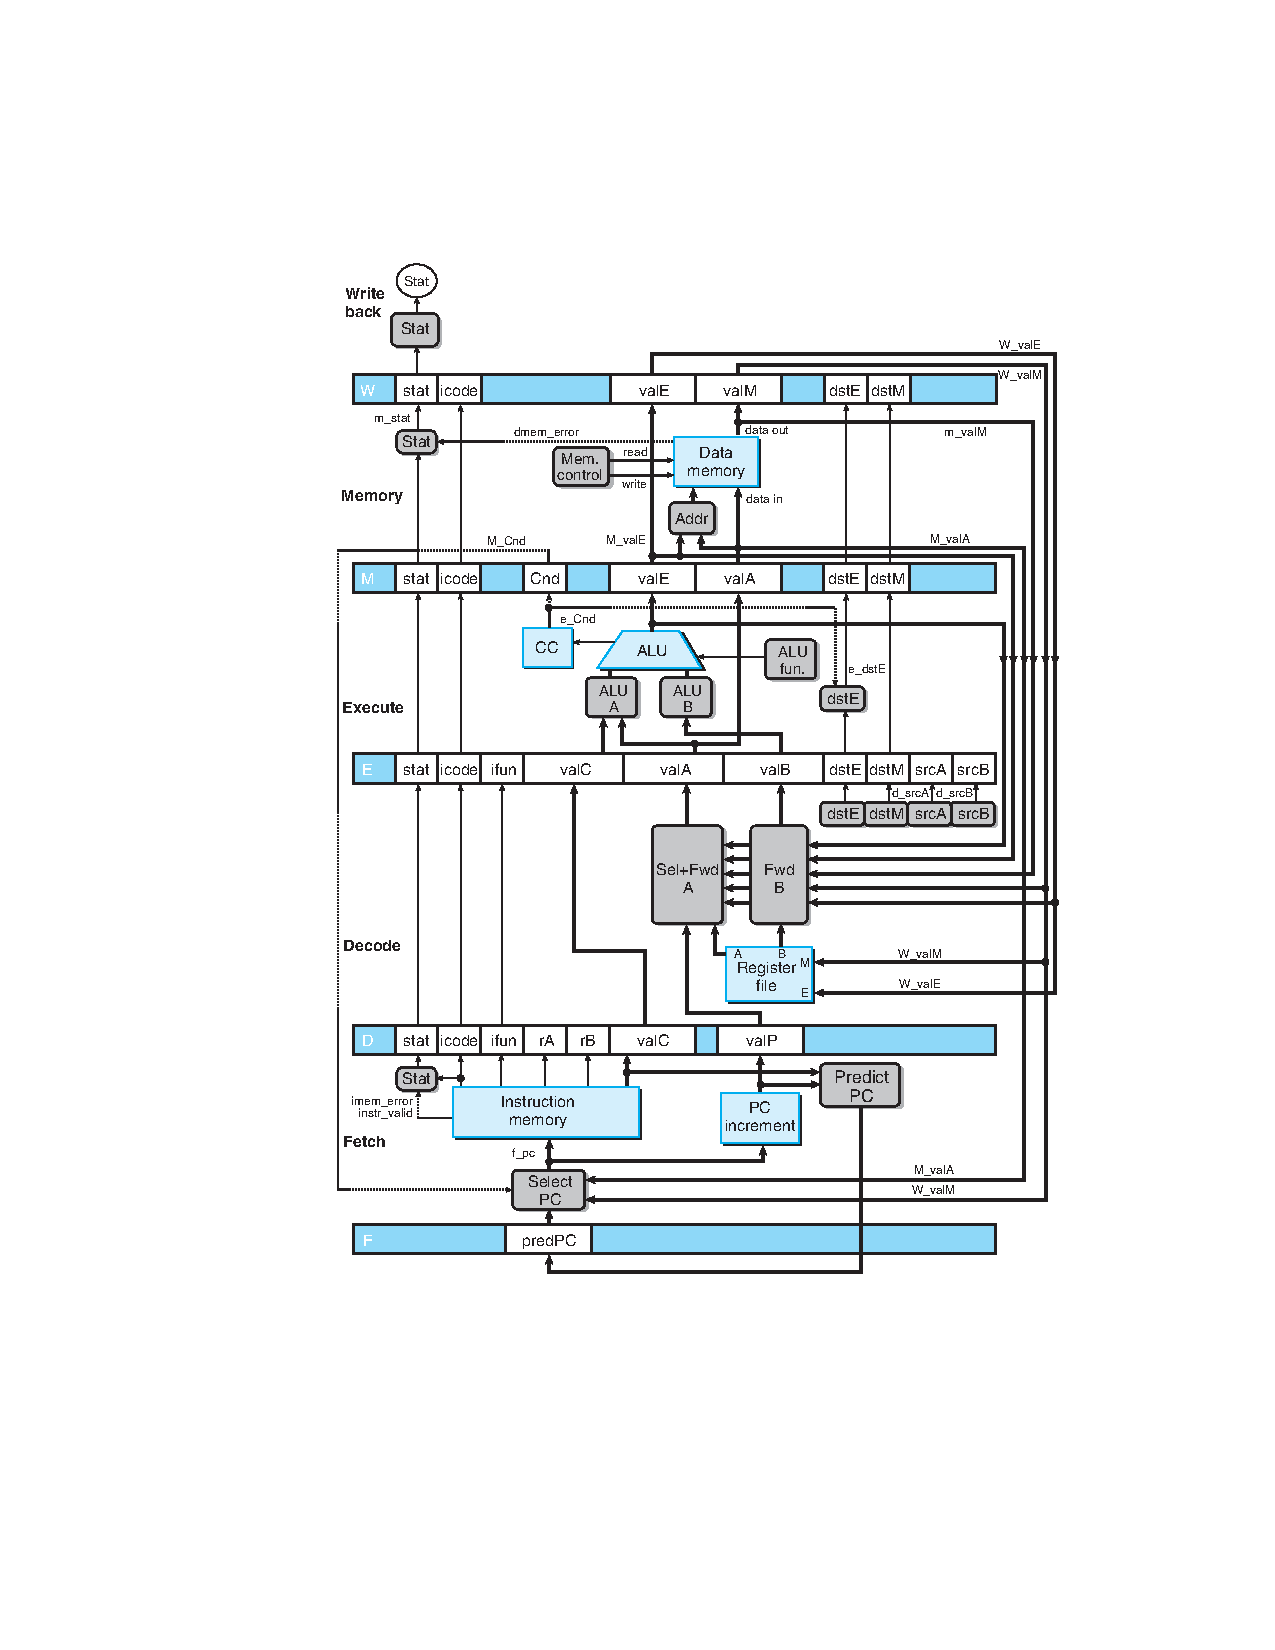
\includegraphics[width=0.75\linewidth]{pipe.pdf}
        \end{figure}
            \qn 该处理器设计采用了前递(forwarding)技术,一定程度上解决了数据相关的问题,在上图中体现在 Sel+FwdA 和 FwdB 部件上。前者输出的信号会存到流水线寄存器 E 的 \verb|valA| 域(即 \verb|E_valA| 信号),请补全该信号的 HCL 语言描述。
            \begin{minted}[frame=single, fontsize=\small]{text}
    int E_valA = [
        D_icode in { ICALL, IJXX } : _________________;
        d_srcA == e_dstE : _________________;
        d_srcA == M_dstM : _________________;
        d_srcA == M_dstE : M_valE;
        d_srcA == W_dstM : W_valM;
        ...
    ];
            \end{minted}
            \qn 如果在该处理器上运行下面的程序,每条指令在不同时钟周期所处的流水线阶段如下表所示。在这种情况下,哪条指令的执行结果会有错误?写出该指令的地址 \rule{2.5cm}{0.25mm}。
            \begin{table}[H]
                \centering
                \begin{tabular}{l|c|c|c|c|c|c|c|c|c|c|c|}
                    \cline{2-12}
                    & 1 & 2 & 3 & 4 & 5 & 6 & 7 & 8 & 9 & 10 & 11 \\ \cline{2-12} 
                    \verb|0x000: irmovl $128, %edx| & F & D & E & M & W &  &  &  &  &  &  \\ \cline{2-12} 
                    \verb|0x006: irmovl $3, %ecx| &  & F & D & E & M & W &  &  &  &  &  \\ \cline{2-12} 
                    \verb|0x00c: rmmovl %ecx, 0(%edx)| &  &  & F & D & E & M & W &  &  &  &  \\ \cline{2-12} 
                    \verb|0x012: irmovl $10, %ebx| &  &  &  & F & D & E & M & W &  &  &  \\ \cline{2-12} 
                    \verb|0x018: mrmovl 0(%edx),%eax| &  &  &  &  & F & D & E & M & W &  &  \\ \cline{2-12} 
                    \verb|0x01e: addl %ebx, %eax| &  &  &  &  &  & F & D & E & M & W &  \\ \cline{2-12} 
                    \verb|0x020: halt| &  &  &  &  &  &  & F & D & E & M & W \\ \cline{2-12} 
                \end{tabular}
            \end{table}
            \qn 如需检测出这个情况,需要增加逻辑电路,用 HCL 语言表达如下:
            \begin{minted}[frame=single, fontsize=\small]{text}
    E_icode in {IMRMOVL, IPOPL} && __________  in { __________ }
            \end{minted}
            \qn 当新增的电路检测出这个情况后,应对各流水线寄存器进行不同的设置,以便在尽可能少影响性能的前提下解决该问题。请填写下表,可选的设置包括 normal/bubble/stall 三种。
            \begin{table}[H]
                \centering
                \begin{tabular}{|c|c|c|c|c|}
                    \hline
                    F & D & E & M & W \\ \hline
                    {\qquad \qquad} & {\qquad \qquad} & {\qquad \qquad} & {\qquad \qquad} & {\qquad \qquad} \\ \hline
                \end{tabular}
            \end{table}
            \qn 如果遇到下面程序代码所展示的情况,该处理器运行时仍然存在问题。因此,还需要新增检测电路。当新增的电路检测出这个情况后,应对各流水线寄存器进行不同的设置,以便在尽可能少影响性能的前提下解决该问题。请填写下表,可选的设置包括 normal/bubble/stall 三种。
            \begin{minted}[frame=single, fontsize=\small]{text}
    0x018: rmmovl   %ecx,0(%edx)
    0x01e: irmovl   $10, %ebx
    0x024: popl     %esp
    0x026: ret
            \end{minted}
            \begin{table}[H]
                \centering
                \begin{tabular}{|c|c|c|c|c|}
                    \hline
                    F & D & E & M & W \\ \hline
                    {\qquad \qquad} & {\qquad \qquad} & {\qquad \qquad} & {\qquad \qquad} & {\qquad \qquad} \\ \hline
                \end{tabular}
            \end{table}
        \proy{2018} Y86 指令 \verb|popl rA| 的 SEQ 实现中,在取指阶段,\verb|valP <- |(\quad),在执行阶段,\verb|valE <- |(\quad)。
        \begin{choices}
            \item \verb|PC+4|、\verb|valA+4|
            \item \verb|PC+4|、\verb|valA+(-4)|
            \item \verb|PC+2|、\verb|valB+4|
            \item \verb|PC+2|、\verb|valB+(-4)|
        \end{choices}
        \proy{2018} 假设已有声明
        \begin{center}
            \tt int i, int sum, int *p, int *q, int *r,const int n = 100, float a[n], float b[n], float c[n], int foo(int), void bar()
        \end{center}
        以下哪项程序优化编译器总是可以进行?
        \vspace{\baselineskip}
        \begin{choices}
            \item \begin{minted}[frame=single, fontsize=\small, linenos]{c}
    // 优化前
    for(i = 0; i < n; ++i) { a[i] += b[i]; a[i] += c[i]; }
    // 优化后
    float tmp;
    for(i = 0; i < n; ++i) { tmp = b[i] + c[i]; a[i] += tmp; }
            \end{minted}
            \item \begin{minted}[frame=single, fontsize=\small, linenos]{c}
    // 优化前
    *p += *q; *p += *r;
    // 优化后
    int tmp;
    tmp = *q + *r;
    *p += tmp;
            \end{minted}
            \item \begin{minted}[frame=single, fontsize=\small, linenos]{c}
    // 优化前
    for(i = 0; i < n; ++i) sum += i * 4;
    // 优化后
    int N = n * 4;
    for(i = 0; i < N; i += 4) sum += i;
            \end{minted}
            \item \begin{minted}[frame=single, fontsize=\small, linenos]{c}
    // 优化前
    for(i = 0; i < foo(n); ++i) bar();
    // 优化后
    int tmp = foo(n);
    for(i = 0; i < tmp; ++i) bar();
            \end{minted}
        \end{choices}
        \proy{2018} 在 PIPE 处理器上运行如下 Y86 代码
        \begin{minted}[frame=single, fontsize=\small]{text}
    .L1
        mrmov   (%eax) %ebx
        addl    %ebx, %ecx
        addl    %ecx, %eax
        xorl    %ecx, %edx
        jne     .L1
        irmov   $1, %eax
        irmov   $1, %eax
        \end{minted}
            \qn 假设上述代码一共循环执行了 $N$ 次后跳出循环,未采用数据前递(data forwarding),分支每次都预测正确,访存每次都命中缓存,命中缓存 时访存需要 1 个周期。请问共需执行多少个周期?
            \qn 假设上述代码一共循环执行了 $N$ 次后跳出循环,采用数据前递(data forwarding),分支每次都预测跳转(taken),访存每次都命中缓存,命中缓存时访存需要 1 个周期。请问共需执行多少个周期?
            \qn 假设上述代码一共循环执行了 $N$ 次后跳出循环($N$ 为偶数),采用数据前递(data forwarding),分支每次都预测不跳转(not taken),数据访存时缓存命中率为 50\%,指令访存全部命中缓存,命中缓存时访存需要 1 个周期,未命中缓存时访存需要 3 个周期。请问共需执行多少个周期?
        \proy{2017} 在 Y86 的 SEQ 实现中,对仅考虑 \verb|IRMMOVQ|、\verb|ICALL|、\verb|IPOPQ|、\verb|IRET| 指令, 对 \verb|mem_addr| 的 HCL 描述正确的是:
        \begin{minted}[frame=single, fontsize=\small]{text}
    word mem_addr = [
        icode in { (1), (2) } : valE;
        icode in { (3), (4) } : valA;
    ];
        \end{minted}
        \begin{choices}
            \item \verb|(1) IRMMOVQ  (2) IPOPQ  (3) IRET     (4) ICALL|
            \item \verb|(1) IRMMOVQ  (2) IRET   (3) IPOPQ    (4) ICALL|
            \item \verb|(1) ICALL    (2) IPOPQ  (3) IRMMOVQ  (4) IRET|
            \item \verb|(1) IRMMOVQ  (2) ICALL  (3) IPOPQ    (4) IRET|
        \end{choices}
        \proy{2017} 关于流水线技术的描述,错误的是: 
        \begin{choices}
            \item 流水线技术能够提高执行指令的吞吐率,但也同时增加单条指令的执行时间。
            \item 增加流水线级数,不一定能获得总体性能的提升。
            \item 指令间数据相关引发的数据冒险,不一定可以通过暂停流水线来解决。
            \item 流水级划分应尽量均衡,吞吐率会受到最慢的流水级影响,均衡的流水线能提高吞吐量。
        \end{choices}
        \proy{2017} 分析 64 位的 Y86 ISA 中新加入的条件内存传送指令:\verb|crmmovqXX| 和 \verb|cmrmovqXX|。\verb|crmmovqXX| 和 \verb|cmrmovqXX| 指令在条件码满足所需要的约束时,分别执行和 \verb|rmmovq| 以及 \verb|mrmovq| 同样的语义。其格式如下:
        \begin{table}[H]
            \tt
            \centering
            \begin{tabular}{c|c|c|c|c|c|}
                \cline{2-6}
                rmmovq & 4 & 0 & rA & rB & D (8 bytes) \\ \cline{2-6} 
                crmmovqXX & 4 & fn & rA & rB & D (8 bytes) \\ \cline{2-6} 
                mrmovq & 5 & 0 & rA & rB & D (8 bytes) \\ \cline{2-6} 
                cmrmovqXX & 5 & fn & rA & rB & D (8 bytes) \\ \cline{2-6} 
            \end{tabular}
        \end{table}
        \qn 请按下表补全每个阶段的操作。需说明的信号可能会包括:\verb|icode|、\verb|ifun|、\verb|rA|、\verb|rB|、\verb|valA|、\verb|valB|、\verb|valC|、\verb|valE|、\verb|valP|、\verb|Cnd|;寄存器堆 \verb|R[]|、存储器 \verb|M[]|、程序计数器 \verb|PC|、条件码 \verb|CC|。其中对存储器的引用必须标明字节数。
        \begin{table}[H]
            \centering
            \begin{tabular}{|c|c|c|}
                \hline
                阶段 & {\qquad} \verb|rmmovq rA, D(rB)| {\qquad} & {\qquad} \verb|cmrmovqXX D(rB), rA| {\qquad} \\ \hline
                取指 & \multicolumn{2}{c|}{\rule{0pt}{8ex}} \\ \hline
                译码 & \multicolumn{2}{c|}{\texttt{valA <- R[rA], valB <- R[rB]}} \\ \hline
                执行 & \rule{0pt}{8ex} & \rule{0pt}{8ex} \\ \hline
                访存 & \rule{0pt}{8ex} & \rule{0pt}{8ex} \\ \hline
                写回 & N/A & \rule{0pt}{8ex} \\ \hline
                更新 \verb|PC| & \multicolumn{2}{c|}{\texttt{PC <- valP}} \\ \hline
            \end{tabular}
        \end{table}
        \qn 为了执行上述新增指令,我们需要改进教材所描述的 PIPE 处理器,在回写(W: Write Back)阶段引入寄存器以保持流水线信号 \rule{2.5cm}{0.25mm} (请参考教材对信号的命名规则书写),以便有条件地更新寄存器内容。在如此改进的 PIPE 处理器上,请写出如下信号的 HCL 代码。
        \begin{minted}[frame=single, fontsize=\small]{text}
    // F_stall 的 HCL 代码:
    (E_icode in {IMRMOVQ, IPOPQ} || (_____1_____))
        && E_dstM in _____2_____ || IRET in _____3_____
    // E_bubble 的 HCL 代码:
    (_____4_____) || (E_icode in {IMRMOVQ, IPOPQ}
        || (_____1_____)) && E_dstM in _____2_____
    // M_bubble 的 HCL 代码:
    m_stat in _____5_____ || W_stat in _____5_____
        \end{minted}
        \qn 对于下面的 Y86 汇编代码,请使用上述条件内存传送指令将其修改为不带跳转的汇编代码序列。假设下面的代码片段在教材所描述的 PIPE 处理器上运行,不考虑该片段前后代码的影响以及高速缓存(cache)失效的情况,假设 \verb|%rsi| 初值为 0, 处理器设计使用总是选择(always taken)的预测策略。原始代码片段预计运行 \rule{2.5cm}{0.25mm} 周期,改进代码片段预计执行 \rule{2.5cm}{0.25mm} 周期。
        \begin{minted}[frame=single, fontsize=\small]{text}
        andq    %rsi %rsi
        jne     L1
        mrmovq  8(%rdx), %rax
        j       L2
    L1:
        mrmovq  8(%rdx), %rbx
    L2:
        addq    %rax, %rbx
        \end{minted}
        \sol 取指部分的填法是很基本的,需要获得 \verb|rA, rB, D|,所以我们写 \verb|icode:ifun <- M1[PC]|、 \verb|rA:rB <- M1[PC+1]|、\verb|valC <- M8[PC+2]| 和 \verb|vavlP <- PC+10|。译码部分也很简单,为 \verb|valA <- R[rA]|、\verb|valB <- R[rB]|。
        
        在执行部分,\verb|rmmovq| 都要计算地址偏移,因此 \verb|valE <- valB+valC|,但是 \verb|cmrmovqXX| 还需要处理条件码,所以还要填 \verb|Cnd <- Cond(CC, ifun)|。最后 \verb|rmmovq| 还需要访存,即 \verb|M8[valE] <- valA|;而 \verb|cmrmovqXX| 除了访存 \verb|valM <- M8[valE]| 之外,还需要条件写回 \verb|if (Cnd) R[rA] <- valM|。
        \proy{2016} 下面对指令系统的描述中,错误的是:
        \begin{choices}
            \item CISC 指令系统中的指令数目较多,有些指令的执行周期很长;而 RISC 指令系统中通常指令数目较少,指令的执行周期都较短。
            \item CISC 指令系统中的指令编码长度不固定;RISC 指令系统中的指令编码长度固定,这样使得 CISC 机器可以获得了更短的代码长度。
            \item CISC指令系统支持多种寻址方式,RISC指令系统支持的寻址方式较少。
            \item CISC 机器中的寄存器数目较少,函数参数必须通过栈来进行传递;RISC 机器中的寄存器数目较多,只需要通过寄存器来传递参数,避免了不必要的存储访问。
        \end{choices}
        \proy{2016} 下面对流水线技术的描述,正确的是:
        \begin{choices}
            \item 流水线技术不仅能够提高执行指令的吞吐率,还能减少单条指令的执行时间。
            \item 不断加深流水线级数,总能获得性能上的提升。
            \item 流水级划分应尽量均衡,吞吐率会受到最慢的流水级影响。
            \item 指令间的数据相关可能会引发流水线停顿,但总是可以通过调度指令来解决。
        \end{choices}
        \proy{2016} 若处理器实现了三级流水线,每一级流水线实际需要的运行时间分别为 \SI{1}{ns}、\SI{2}{ns} 和 \SI{3}{ns},则此处理器不停顿地执行完毕 10 条指令需要的时间为:
        \begin{choices}
            \item \SI{21}{ns}
            \item \SI{12}{ns}
            \item \SI{24}{ns}
            \item \SI{36}{ns}
        \end{choices}
        \sol 首先,每级流水线都是 \SI{3}{ns},然后画出时序图就可以了。一般地,需要时间是一级流水线的总时间,补上一头一尾。这里需要的时间为 $10 \times 3+3+3 = \SI{36}{ns}$。
        \proy{2016} 假设流水线数据通路中的转移预测策略为总是预测跳转。如果转移预测错误,需要恢复流水线,并从正确的目标地址开始取值。其中用来判断转移预测是否正确的信号是 \rule{2.5cm}{0.25mm} 和 \rule{2.5cm}{0.25mm},用来获得正确的目标地址的信号是 \rule{2.5cm}{0.25mm}。
        \begin{choices}
            \item \verb|M_icode   M_Bch   M_valA|
            \item \verb|W_icode   M_Bch   M_valA|
            \item \verb|W_icode   M_Bch   W_valM|
            \item \verb|M_icode   M_Bch   W_valM|
        \end{choices}
        \proy{2016} 请分析 32 位的 Y86 ISA 中新加入的一组条件返回指令 \verb|cretXX|,其格式如下。
        \begin{table}[H]
            \tt
            \centering
            \begin{tabular}{c|c|c|}
                \cline{2-3}
                cretXX & 9 & fun \\ \cline{2-3} 
            \end{tabular}
        \end{table}
        类似 \verb|cmovXX|,该组指令只有当条件码 \verb|Cnd| 满足时,才执行函数返回;如果条件不满足,则顺序执行。
        \qn 若在教材所描述的 SEQ 处理器上执行这条指令,请按下表补全每个阶段的操作。需说明的信号可能会包括:\verb|icode|、\verb|ifun|、\verb|rA|、\verb|rB|、\verb|valA|、\verb|valB|、\verb|valC|、\verb|valE|、\verb|valP|、\verb|Cnd|;寄存器堆 \verb|R[]|、存储器 \verb|M[]|、程序计数器 \verb|PC|、条件码 \verb|CC|。其中对存储器的引用必须标明字节数。如果在某一阶段没有任何操作,请填写 \texttt{none} 指明。
        \begin{table}[H]
            \centering
            \begin{tabular}{|c|c|}
                \hline
                阶段 & {\qquad \qquad \qquad \qquad} \verb|cretXX offset| {\qquad \qquad \qquad \qquad} \\ \hline
                取指 & \rule{0pt}{8ex} \\ \hline
                译码 & \rule{0pt}{8ex} \\ \hline
                执行 & \rule{0pt}{8ex} \\ \hline
                访存 & \rule{0pt}{8ex} \\ \hline
                写回 & \rule{0pt}{8ex} \\ \hline
                更新 \verb|PC| & \rule{0pt}{8ex} \\ \hline
            \end{tabular}
        \end{table}
        \qn 为了执行 \verb|cretXX| 指令,我们需要改进教材所描述的 PIPE 处理器,在 W(Write Back)阶段引入流水线寄存器 \rule{2.5cm}{0.25mm},并将其连接到 PC 选择器(Select PC)以便有条件地更新 PC。假设改进后的处理器总是预测函数返回条件不满足,则如果返回条件满足时,一共会错误取指 \rule{2.5cm}{0.25mm} 条指令。
        \qn 在(2)中改进的 PIPE 处理器上执行 \verb|cretXX| 指令时,发生预测错误时的判断条件为:
        \begin{minted}[frame=single, fontsize=\small]{text}
    (______________ = ICRETXX && ______________) ||
        (______________ = ICRETXX && ______________)
        \end{minted}
        此时各级流水线寄存器的控制信号应如何设置?填写下表。
        \begin{table}[H]
            \centering
            \begin{tabular}{|c|c|c|c|c|}
                \hline
                F & D & E & M & W \\ \hline
                {\qquad \qquad} & {\qquad \qquad} & {\qquad \qquad} & normal & normal \\ \hline
            \end{tabular}
        \end{table}
        \qn 若在 PIPE 处理器上处理器上执行如下代码片段:
        \begin{minted}[frame=single, fontsize=\small]{text}
    0x000: xorl   %eax, %eax
    0x002: popl   %esp
    0x004: cretne
        \end{minted}
            \subqn 是否会发生 load-use 和 misprediction cret 组合的 hazard 情况?
            \subqn 如果此时 \verb|popl %esp| 指令处在流水线的 Execute 阶段,请问此时各级流水线寄存器的控制信号应如何设置?填写下表。
            \begin{table}[H]
                \centering
                \begin{tabular}{|c|c|c|c|c|}
                    \hline
                    F & D & E & M & W \\ \hline
                    {\qquad \qquad} & {\qquad \qquad} & {\qquad \qquad} & normal & normal \\ \hline
                \end{tabular}
            \end{table}
        \sol 本质还是 \verb|ret|,只是需要稍微添加一下条件判断。取指是 \verb|icode:ifun <- M1[PC]|、\verb|valP <- PC+1|。译码需要注意,在 \verb|ret| 中两个值都会被取用,故填写 \verb|valB <- R[%rsp]|、\verb|valA <- R[%rsp]|。
        
        执行阶段是要恢复栈空间,因此为 \verb|valE <- valB+4| 和 \verb|Cnd <- Cond(CC, ifun)|。这里用 \verb|valA| 也可以。访存阶段需要读出返回地址,请注意,这里必须用 \verb|valA|(参看SEQ 实现图中的数据通路),填写 \verb|valM <- M4[valA]|。随后的写回和更新程序计数器的工作主要是关心条件(是否真的要返回了),所以分别是 \verb|if (Cnd) R[%rsp] <- valE| 和 \verb|PC <- Cnd?valM:valP|。
        \proy{2015} 下面有关指令系统设计的描述正确的是:
        \begin{choices}
            \item 采用 CISC 指令比 RISC 指令代码更长。
            \item 采用 CISC 指令比 RISC 指令运行时间更短。
            \item 采用 CISC 指令比 RISC 指令译码电路更加复杂。
            \item 采用 CISC 指令比 RISC 指令的流水线吞吐更高。
        \end{choices}
        \proy{2015} 一个功能模块包含组合逻辑和寄存器,组合逻辑单元的总延迟是 \SI{100}{ps},单个寄存器的延时是 20ps,该功能模块执行一次并保存执行结果,理论上能达到的最短延时和最大吞吐分别是多少?
        \begin{choices}
            \item \SI{20}{ns}、\SI{50}{GIPS}
            \item \SI{120}{ns}、\SI{50}{GIPS}
            \item \SI{120}{ns}、\SI{10}{GIPS}
            \item \SI{20}{ps}、\SI{10}{GIPS}
        \end{choices}
        \proy{2015} 关于流水线技术的描述,错误的是:
        \begin{choices}
            \item 流水线技术能够提高执行指令的吞吐率,但也同时增加单条指令的执行时间。
            \item 减少流水线的级数,能够减少数据冒险发生的几率。
            \item 指令间数据相关引发的数据冒险,都可以通过数据转发来解决。
            \item 现代处理器支持一个时钟内取指、执行多条指令,会增加控制冒险的开销。
        \end{choices}
        \proy{2015} 以下哪些程序优化编译器总是可以自动进行?假设
        \begin{center}
            \tt int i, int j, int A[N], int B[N], float m
        \end{center}
        都是局部变量,\verb|N| 是一个整数型常量,\verb|int foo(int)| 是一个函数。
        \vspace{\baselineskip}
        \begin{choices}
            \item \begin{minted}[frame=single, fontsize=\small, linenos]{c}
    // 优化前
    for (j = 0; j < N; j++) m += i * N * j;
    // 优化后
    int temp = i * N;
    for (j = 0; j < N; j++) m += temp * j;
            \end{minted}
            \item \begin{minted}[frame=single, fontsize=\small, linenos]{c}
    // 优化前
    for (j = 0; j < N; j++) B[i] *= A[j];
    // 优化后
    int temp = B[i];
    for (j = 0; j < N; j++) temp *= A[j];
    B[i] = temp;
            \end{minted}
            \item \begin{minted}[frame=single, fontsize=\small, linenos]{c}
    // 优化前
    for(j = 0; j < N; j++) m = (m + A[j]) + B[j];
    // 优化后
    for(j = 0; j < N; j++) m = m + (A[j] + B[j]);
            \end{minted}
            \item \begin{minted}[frame=single, fontsize=\small, linenos]{c}
    // 优化前
    for(j = 0; j < foo(N); j++) m++;
    // 优化后
    int temp = foo(N);
    for(j = 0; j < temp; j++) m++;
            \end{minted}
        \end{choices}
        \proy{2015} 请分析 Y86 ISA 中新加入的一条指令:\verb|NewJE|,其格式如下。
        \begin{table}[H]
            \centering
            \begin{tabular}{c|c|c|c|c|c|}
                \cline{2-6}
                NewJE & C & 0 & rA & rB & dst \\ \cline{2-6} 
            \end{tabular}
        \end{table}
        其功能为:如果 \verb|R[rA] = R[rB]|,则跳转到 \verb|dst| 继续执行,否则顺序执行。
        \qn 若在教材所描述的 SEQ 处理器上执行这条指令,请按下表补全每个阶段的操作。需说明的信号可能会包括:\verb|icode|、\verb|ifun|、\verb|rA|、\verb|rB|、\verb|valA|、\verb|valB|、\verb|valC|、\verb|valE|、\verb|valP|、\verb|Cnd|;寄存器堆 \verb|R[]|、存储器 \verb|M[]|、程序计数器 \verb|PC|、条件码 \verb|CC|。其中对存储器的引用必须标明字节数。如果在某一阶段没有任何操作,请填写 \texttt{none} 指明。
        \begin{table}[H]
            \centering
            \begin{tabular}{|c|c|}
                \hline
                阶段 & {\qquad \qquad \qquad \qquad} \verb|cretXX offset| {\qquad \qquad \qquad \qquad} \\ \hline
                取指 & \rule{0pt}{8ex} \\ \hline
                译码 & \rule{0pt}{8ex} \\ \hline
                执行 & \rule{0pt}{8ex} \\ \hline
                访存 & \rule{0pt}{8ex} \\ \hline
                写回 & \rule{0pt}{8ex} \\ \hline
                更新 \verb|PC| & \rule{0pt}{8ex} \\ \hline
            \end{tabular}
        \end{table}
        \qn 若在教材所描述的 PIPE 处理器上执行 \verb|NewJE| 指令,如果跳转条件不满足,一共会错误执行 \rule{2.5cm}{0.25mm} 条指令。
        
        为了减小错误预测的代价,现将教材所描述的 PIPE 处理器做如下改进:在 Decode 阶段增加一个比较器,用于判断 \verb|R[rA] = R[rB]| 条件,比较器的输出信号为 \verb|d_equal|。如果相等,则 \verb|d_equal = 1|,反之 \verb|d_equal = 0|。此时,如果执行 \verb|NewJE| 指令时跳转条件不满足,一共会错误执行 \rule{2.5cm}{0.25mm} 条指令。
        \qn 已知在教材所描述的 PIPE 处理器上执行 \verb|jXX| 指令时,发生转移预测错误的判断条件和此时各级流水线寄存器的控制信号如下所示:
        \begin{minted}[frame=single, fontsize=\small]{text}
    E_icode = IJXX & !e_Cnd
        \end{minted}
        \begin{table}[H]
            \centering
            \begin{tabular}{|c|c|c|c|c|}
                \hline
                F & D & E & M & W \\ \hline
                normal & bubble & bubble & normal & normal \\ \hline
            \end{tabular}
        \end{table}
        据此,在第(2)小题所述的改进后的处理器上执行 \verb|NewJE| 指令,发生转移预测错误的判断条件和此时各级流水线寄存器的控制信号应如何设置?
        \begin{minted}[frame=single, fontsize=\small]{text}
    ______________ = INewJE && ______________
        \end{minted}
        \begin{table}[H]
            \centering
            \begin{tabular}{|c|c|c|c|c|}
                \hline
                F & D & E & M & W \\ \hline
                {\qquad \qquad} & {\qquad \qquad} & {\qquad \qquad} & {\qquad \qquad} & {\qquad \qquad} \\ \hline
            \end{tabular}
        \end{table}
        \qn 在第(2)小题所述的改进后的处理器上执行如下代码:
        \begin{minted}[frame=single, fontsize=\small]{text}
    0x000: mrmovl   0(%eax), %edx
    0x006: NewJE    %edx, %eax, t
    0x00c: irmovl   $1, %eax       # Fall through
    0x012: nop
    0x013: nop
    0x014: nop
    0x015: halt
    0x016: t:  irmovl $3, %edx     # Target (Should not execute)
    0x01c: irmovl   $4, %ecx       # Should not execute
    0x022: irmovl   $5, %edx       # Should not execute
        \end{minted}
        会发生 load-use 和 misprediction 组合的 hazard 情况。请问此时,各级流水线寄存器的控制信号应如何设置?
        \begin{table}[H]
            \centering
            \begin{tabular}{|c|c|c|c|c|}
                \hline
                F & D & E & M & W \\ \hline
                {\qquad \qquad} & {\qquad \qquad} & {\qquad \qquad} & normal & normal \\ \hline
            \end{tabular}
        \end{table}
        \qn 在教材 PIPE 处理器设计中,data memory 实际是高速缓存(cache)。假设在执行上述(4)中代码时,\verb|0x000| 指令中的 \verb|0(%eax)| 地址中的数据不在 data memory 中,则 data memory 会将输出信号 \verb|m_datamiss| 置为 1,直到数据从内存中取回到 data memory,再将 \verb|m_datamiss| 置为 0。设 \verb|m_datamiss| 的默认值为 0。这种情况的判断条件如下,请问各级流水线寄存器的控制信号应如何设置?
        \begin{minted}[frame=single, fontsize=\small]{text}
    M_icode in { IMRMOVL, IPOPL } && m_datamiss
        \end{minted}
        \begin{table}[H]
            \centering
            \begin{tabular}{|c|c|c|c|c|}
                \hline
                F & D & E & M & W \\ \hline
                {\qquad \qquad} & {\qquad \qquad} & {\qquad \qquad} & {\qquad \qquad} & {\qquad \qquad} \\ \hline
            \end{tabular}
        \end{table}
        \proy{2014} 若处理器实现了三级流水线,每一级流水线实际需要的运行时间分别为 \SI{2}{ns}、\SI{2}{ns} 和 \SI{1}{ns},则此处理器不停顿地执行完毕 10 条指令需要的时间为:
        \begin{choices}
            \item \SI{21}{ns}
            \item \SI{22}{ns}
            \item \SI{23}{ns}
            \item \SI{24}{ns}
        \end{choices}
        \proy{2014} 关于 RISC 和 CISC 的描述,正确的是:
        \begin{choices}
            \item CISC 指令系统的指令编码可以很短,例如最短的指令可能只有一个字节,因此 CISC 的取指部件设计会比 RISC 更为简单。
            \item CISC 指令系统中的指令数目较多,因此程序代码通常会比较长;而 RISC 指令系统中通常指令数目较少,因此程序代码通常会比较短。
            \item CISC 指令系统支持的寻址方式较多,RISC 指令系统支持的寻址方式较少,因此用 CISC 在程序中实现访存的功能更容易。
            \item CISC 机器中的寄存器数目较少,函数参数必须通过栈来进行传递;RISC 机器中的寄存器数目较多,只需要通过寄存器来传递参数。
        \end{choices}
        \proy{2014} 关于流水线技术的描述,正确的是:
        \begin{choices}
            \item 指令间数据相关引发的数据冒险,一定可以通过暂停流水线来解决。
            \item 流水线技术不仅能够提高执行指令的吞吐率,还能减少单条指令的执行时间。
            \item 增加流水线的级数,一定能获得性能上的提升。
            \item 流水级划分应尽量均衡,不均衡的流水线会增加控制冒险。
        \end{choices}
        \proy{2014} 下面关于程序性能的说法中,哪个是正确的?
        \begin{choices}
            \item 处理器内只要有多个功能部件空闲,就能实现指令并行,从而提高程序性能。
            \item 同一个任务采用时间复杂度为 $O(\log N)$ 算法一定比采用复杂度为 $O(N)$ 算法的执行时间短。
            \item 转移预测总是能带来好处,不会产生额外代价,对提高程序性能有帮助。
            \item 增大循环展开(loop unrolling)的级数,有可能降低程序的性能(即增加执行时间)。
        \end{choices}
        \proy{2014} 请分析 Y86 ISA 中新加入的一条指令:\verb|caddXX| 条件加法。其功能可以参考 \verb|add| 和 \verb|cmovXX| 两条指令。
        \begin{table}[H]
            \centering
            \begin{tabular}{c|c|c|c|c|}
                \cline{2-5}
                caddXX & C & fn & rA & rB \\ \cline{2-5} 
            \end{tabular}
        \end{table}

        若在教材所描述的 SEQ 处理器上执行这条指令,请按下表补全每个阶段的操作。需说明的信号可能会包括:\verb|icode|、\verb|ifun|、\verb|rA|、\verb|rB|、\verb|valA|、\verb|valB|、\verb|valC|、\verb|valE|、\verb|valP|、\verb|Cnd|;寄存器堆 \verb|R[]|、存储器 \verb|M[]|、程序计数器 \verb|PC|、条件码 \verb|CC|。其中对存储器的引用必须标明字节数。如果在某一阶段没有任何操作,请填写 \texttt{none} 指明。
        \begin{table}[H]
            \centering
            \begin{tabular}{|c|c|}
                \hline
                阶段 & {\qquad \qquad \qquad \qquad} \verb|caddXX offset| {\qquad \qquad \qquad \qquad} \\ \hline
                取指 & \rule{0pt}{8ex} \\ \hline
                译码 & \rule{0pt}{8ex} \\ \hline
                执行 & \rule{0pt}{8ex} \\ \hline
                访存 & \rule{0pt}{8ex} \\ \hline
                写回 & \rule{0pt}{8ex} \\ \hline
                更新 \verb|PC| & \rule{0pt}{8ex} \\ \hline
            \end{tabular}
        \end{table}
    \end{problems}
	\chapter{存储器层次结构}\thispagestyle{empty}
    \begin{summary}
        \begin{compactitem}
            \item 了解 SRAM、DRAM 等易失性存储器及其变种(如 DDR SDARM 等)的功能和历史;了解 PROM、EPROM 等非易失性存储器及其变种的功能和历史。
            \item 知道传统旋转磁盘的结构相关概念和工作原理,会计算其存储容量和使用磁盘访问数据的延迟。了解固态硬盘的工作原理。
            \item 了解计算机体系结构中总线的作用以及含总线的计算机基本结构。
            \item 熟悉时间局部性和空间局部性的概念,会阅读程序判断局部性的概念。
        \end{compactitem}
    \end{summary}

    \begin{problems}
        \pro 对于下列描述,是 SRAM 更符合还是 DRAM 更符合,还是均符合?
            \qn 访问速度更快
            \qn 每比特需要的晶体管数目少
            \qn 单位容量造价更便宜
            \qn 常用作主存
            \qn 需要定期刷新
            \qn 断电后失去存储的信息
            \qn 支持随机访问
            \qn 一种变种是 SDRAM
        \sol SRAM 较快,复杂且贵,而 DRAM 相对反之。所以 1 属于 SRAM 而 2、3、4、5 都是 DRAM。6、7 都是 RAM 的属性,而 SDRAM 是一种 DRAM 的变种(SDRAM 是同步动态随机存取存储器的缩写)。
        \pro 下列存储器中,属于易失性存储介质的有:
            \begin{choices}
                \item DRAM
                \item SRAM
                \item ROM
                \item 软盘
                \item SSD
                \item U 盘
            \end{choices}
        \sol AB,属于基本常识题。
        \pro 已知一个双面磁盘有 2 个盘片、10000 个柱面,每条磁道有 400 个扇区,每个扇区容量为 512 字节,则它的存储容量是 \rule{2.5cm}{0.25mm} GB。
        \sol 因为是双面磁盘,所以计算 $2 \times 2 \times 10000 \times 400 \times 512 = \SI{8192000000}{Byte} = \SI{8.192}{GB}$,注意一般较慢的存储介质(例如磁盘容量、网速等)都是用十进制的数前缀。
        \pro 已知一个磁盘的平均寻道时间为 \SI{6}{ms},旋转速度为 \SI{7500}{RPM},那么它的平均访问时间大约为 \rule{2.5cm}{0.25mm} ms。
        \sol 平均地看,需要旋转半周。又磁盘主要的延迟来源于寻道和旋转,所以结果为 $6 + 0.5 \times (60/7500 \times 1000) = \SI{10}{ms}$。
        \pro 已知一个磁盘每条磁道平均有 400 个扇区,旋转速度为 \SI{6000}{RPM},那么它的平均传送时间大约为 \rule{2.5cm}{0.25mm} ms。
        \sol 答案为 $60/6000 \text{ (转一圈的时间)} \times 1/400 \text{ (转过一个磁道的时间)} \times 1000 = \SI{0.025}{ms}$。
        \pro 考虑如下程序:
        \begin{minted}[frame=single, fontsize=\small, linenos]{c}
    for (int i = 0; i < n; i++) {
        B[i] = 0;
        for (int j = 0; j < m; j++)
            B[i] += A[i][j];
    }
        \end{minted}
        判断下列说法的正确性。
            \qn 对于数组 \verb|A| 的访问体现了时间局部性。
            \qn 对于数组 \verb|A| 的访问体现了空间局部性。
            \qn 对于数组 \verb|B| 的访问体现了时间局部性。
            \qn 对于数组 \verb|B| 的访问体现了空间局部性。
        \sol 数组 \verb|A, B| 都存在逐元素访问的过程,因此都体现了空间局部性。但 \verb|B| 存在同一个元素反复访问而 \verb|A| 没有。因此 1 错误而 2、3、4 均正确。顺便一提:任何一个有意义的程序的指令都体现时间局部性(程序计数器)和空间局部性(顺序执行)。
        \pro 回答下列有关缓存结构的问题:
            \qn 一个容量为 \SI{8}{K} 的直接映射高速缓存,每一行的容量为 \SI{32}{B},那么它有 \rule{2.5cm}{0.25mm} 组,每组有 \rule{2.5cm}{0.25mm} 行。
            \qn 一个容量为 \SI{8}{K} 的全相联高速缓存,每一行的容量为 \SI{32}{B},那么它有 \rule{2.5cm}{0.25mm} 组,每组有 \rule{2.5cm}{0.25mm} 行。
            \qn 一个容量为 \SI{16}{K} 的 4 路组相联告诉缓存,每一行的容量为 \SI{64}{B},那么一个 16 位地址 \verb|0xCAFE| 应映射在第 \rule{2.5cm}{0.25mm} 组内。
        \sol 总容量等于组数乘以路数(行数)乘以块大小,其中直接映射高速缓存路数为 1,而全相联高速缓存的组数为 1。因此第一问为 $2^3 \times 2^10/2^5=256$ 组,1 行;第二问为 1 组,$2^3 \times 2^10/32=256$ 行。对于第三问,组数为 $2^4 \times 2^10/(2^6 \times 4)=64$ 组,所以组索引占据 6 位,偏移量占据 6。所给出的地址为 \verb|1100 1010 1111 1110|,即组索引是 \verb|101011|,即 43。
        \pro 判断下列说法的正确性。
            \qn 保持块大小与路数不变,增大组数,命中率一定不会降低。
            \qn 保持总容量与块大小不变,增大路数,命中率一定不会降低。
            \qn 保持总容量与路数不变,增大块大小,命中率一定不会降低。
            \qn 使用随机替换代替 LRU,期望命中率可能会提高。
        \sol 1 正确,相当于在 cache 中直接增加一组空间。2、3 都错误,由于总容量不变,所以组数都会降低,命中率都可能降低。实际上实验表明,增大路数一般会导致命中率降低,而增大块大小对于不同的访存步长可能造成命中率升高或降低。4 正确,对于某些特定的程序,LRU 的期望性能可能不如随机替换(参看 2018 年期中第 13 题的构造),实验表明在较小的 cache 中随机策略更优。
        \pro 考虑如下程序:
        \begin{minted}[frame=single, fontsize=\small, linenos]{c}
    int A[MAXN];
    for (int i = 0; i < 25; i++) {
        int x = A[i];
        int y = A[i + 1];
        int z = A[i + 2];
        A[i + 3] = x + y + z;
    }
        \end{minted}
        假设上述代码编译成汇编语言的时候没有任何优化,变量 \verb|x|、\verb|y|、\verb|z| 均放在寄存器中。系统的高速缓存采用写分配策略,运行之前写 cache 所有行都是无效的。设 \verb|A| 的起始地址为 \verb|0|,且 \verb|MAXN| 充分大,保证没有越界问题。
        \qn 假设 cache 的容量为 8 字节,每一行的容量为 4 字节,替换策略为 LRU,组策略为直接映射高速缓存。在这个 cache 上运行上述代码,得到的 cache 命中率是 \rule{2.5cm}{0.25mm}\%。
        \qn 假设 cache 的容量为 8 字节,每一行的容量为 4 字节,替换策略为 LRU,组策略为全相联高速缓存。在这个 cache 上运行上述代码,得到的 cache 命中率是 \rule{2.5cm}{0.25mm}\%。
        \qn 假设 cache 的容量为 32 字节,每一行的容量为 8 字节,替换策略为 LRU,组策略为 2 路组相联。画出程序运行结束时 cache 的情况(用 \verb|M[0-7]| 表示第 \verb|0| 到第 \verb|7| 字节的地址);cache 命中率是 \rule{2.5cm}{0.25mm}\%。
        \qn 假设 cache 的每一行的容量为 4 字节,运行该程序,得到的 cache 命中率的可能最大值为 \rule{2.5cm}{0.25mm}\%。
        \sol 处理 cache 命中率的题,首先确定 tag, index 和 offset 的分布,然后先尝试通过组索引简化分析,\emph{获得各地址放置位置的规律},最后再直接模拟。对于本题,首先知道每次访问 4 个整数,cache 的每行(路)都能容纳 1 个元素或者 2 个元素(视小问而不同)。一共访存 100 次,只需要计算命中的次数。我们下面用下标 0、1、2、3... 来代指数组中的元素。注意缓存是写分配的,因此即便是写内存也有访问高速缓存的问题(一般我们假设缓存是写分配且写回的)。

        第一问。计算得一共 2 组,每组 1 行,所以最低三位中,高 1 位是组索引,剩下 2 位是偏移。因为是直接映射,且每行只能容纳一个整数,所以组索引其实也代表了元素在数组的下标,因此实际上两行分别存储下标为奇数和偶数的元素。第一次 0、1、2、3 均不命中,此时 2、3 留在缓存中。接着访问 1、2、3、4,但 3 会被 1 替换,只有 2 能命中,结束时 3、4 留在缓存中。再次访问 2、3、4、5,但 4 会被 2 替换,只有 3 能命中。由此发现后 24 组访问各恰有一次命中,命中率为 24\%。

        第二问。计算得只有 1 组,组内有 2 行,因此只有最低 2 位代表组内偏移,每行只能容纳一个整数,因此是依次填满并 LRU 替换。第一次 0、1、2、3 均不命中,此时 2、3 留在缓存中。接着访问 1、2、3、4 时,首先 1 不命中,替换 2,然后 2 不命中,替换 3,最后 4 不命中,替换 2,以此类推。由此发现这个访存序列发生了抖动,每次都不命中,命中率为 0\%。

        第三问需要一些细致的模拟。计算得有 2 组,每组 2 行,每行都能容纳两个连续的整数。在这里,组索引表示的是下标模 4 的结果,也就是说 0、1、4、5... 会进入一组,而 2、3、6、7... 进入另一组。我们预期访存序列模 4 会有某种规律。模拟过程如下(你可能没必要模拟这么长):
        \begin{compactenum}[(i)]
            \item\ 0、1、2、3,其中 0、2 不命中,结束时第一组有 0、1,第二组有 2、3。
            \item\ 1、2、3、4,其中 4 不命中,结束时第一组有 0、1、4、5,第二组有 2、3。
            \item\ 2、3、4、5,全部命中。
            \item\ 3、4、5、6,只有 6 不命中,结束时第一组有 0、1、4、5,第二组有 2、3、6、7。
            \item\ 4、5、6、7,全部命中。
            \item\ 5、6、7、8,只有 8 不命中,此时开始替换,第一组有 8、9、4、5,第二组有 2、3、6、7。
            \item\ 6、7、8、9,全部命中。
            \item\ 7、8、9、10,只有 10 不命中,再次替换,第一组有 8、9、4、5,第二组有 10、11、6、7。
            \item\ 8、9、10、11,全部命中。
            \item\ 9、10、11、12,只有 12 不命中,替换得到第一组有 8、9、12、13,第二组有 10、11、6、7。
        \end{compactenum}
        这样就大致找到规律了,不命中只可能是在 $0, 2, \dotsc, 24, 26$ 时发生,这里一共有 14 次,因此命中率为 86\%。最后一次访存是 24、25、26、27,是全部命中的,根据(iv)、(vi)、(ix)的规律,其中剩下 cache 的部分应该对应前四个元素,即 20\textasciitilde23 都在缓存中。综上所述,地址 \verb|80| 起的 8 个字节都在缓存中,所以缓存可以画为
        \begin{table}[H]
            \tt
            \centering
            \begin{tabular}{|c|c|c|c|c|}
                \hline
                & 有效位 & 内容 & 有效位 & 内容 \\ \hline
                组 0 & 1 & M[96-103] & 1 & M[80-87] \\ \hline
                组 1 & 1 & M[88-95] & 1 & M[104-111] \\ \hline
            \end{tabular}
        \end{table}

        第四问考察冷不命中。当缓存充分大时,至少第一次访问该元素时是要发生不命中的,而这里一共有 28 个元素要访问,所以最高命中率是 72\%。
    \end{problems}

\chapter{存储器层次结构{---}往年考题}\thispagestyle{empty}
    \begin{problems}
        \proy{2018} 以下关于存储的叙述中,正确的是:
        \begin{choices}
            \item 由于基于 SRAM 的内存性能与 CPU 的性能有很大差距,因此现代计算机使用更快的基于 DRAM 的高速缓存,试图弥补 CPU 和内存间性能的差距。
            \item SSD 相对于旋转磁盘而言具有更好的读性能,但是 SSD 写的速度通常比读的速度慢得多,而且 SSD 比旋转磁盘单位容量的价格更贵,此外 SSD 底层基于 EEPROM 的闪存会磨损。
            \item 一个有 2 个盘片,10000 个柱面,每条磁道平均有 400 个扇区,每个扇区有 512 个字节的双面磁盘的容量为 \SI{8}{GB}。
            \item 访问一个磁盘扇区的平均时间主要取决于寻道时间和旋转延迟,因此一个旋转速率为 \SI{6000}{RPM}、平均寻道时间为 \SI{9}{ms} 的磁盘的平均访问时间大约为 \SI{19}{ms}。
        \end{choices}
        \proy{2017} 以下计算机部件中,通常不用于存储器层次结构(Memory Hierarchy)的是:
        \begin{choices}
            \item 高速缓存
            \item 内存
            \item 硬盘
            \item 优盘(U 盘)
        \end{choices}
        \proy{2017} 关于局部性(locality)的描述,正确的是:
        \begin{choices}
            \item 数据的时间局部性或数据空间局部性,在任何有意义的程序中都能体现。
            \item 指令的时间局部性或数据空间局部性,在任何有意义的程序中都能体现。
            \item 数据的时间局部性,在任何循环操作中都能体现。
            \item 数据的空间局部性,在任何数组操作中都能体现。
        \end{choices}
        \proy{2016} 以下关于存储结构的讨论,哪个是正确的?
        \begin{choices}
            \item 增加额外一级存储,数据存取的延时一定不会下降。
            \item 增加存储的容量,数据存取的延时一定不会下降。
            \item 增加额外一级存储,数据存取的延时一定不会增加。
            \item 以上选项都不正确。
        \end{choices}
        \proy{2016} 关于局部性(locality)的描述,不正确的是:
        \begin{choices}
            \item 循环通常具有很好的时间局部性。
            \item 循环通常具有很好的空间局部性。
            \item 数组通常具有很好的时间局部性。
            \item 数组通常具有很好的空间局部性。
        \end{choices}
        \proy{2015} 下面关于存储器的说法,错误的是:
        \begin{choices}
            \item SDRAM 的速度比 FPM DRAM 快。
            \item SDRAM 的 RAS 和 CAS 请求共享相同的地址引脚。
            \item 磁盘的寻道时间和旋转延迟大致在一个数量级。
            \item 固态硬盘的随机读写性能基本相当。
        \end{choices}
        \proy{2015} 某磁盘的旋转速率为 \SI{7200}{RPM},每条磁道平均有 400 扇区,则一个扇区的平均传送时间为 \rule{2.5cm}{0.25mm} ms。
        \proy{2018} 一缓存共包含 4 个缓存块,每个块 32 字节,采用 LRU 替换算法。设缓存初始为空,对其进行下列 \verb|char| 型内存地址序列访存:\verb|0x5a7, 0x5b7, 0x6a6, 0x5b8, 0x7a5, 0x5b9|。对于直接映射缓存和 2 路组相联缓存,分别能产生几次命中?
        \begin{choices}
            \item 1, 3
            \item 1, 4
            \item 2, 3
            \item 2, 4
        \end{choices}
        \proy{2018} 设一种全相联缓存共包含 4 个缓存块,如果循环地顺序访问 5 个不同的内存块(大小和一个缓存块一样),下列哪种替换算法会产生最多的命中?(考虑渐近值即可)
        \begin{choices}
            \item 最近最少使用替换策略 LRU
            \item 先入先出替换策略 FIFO
            \item 随机替换策略 Random
            \item 后入先出替换策略 LIFO
        \end{choices}
        \sol CD。对于全相联缓存,操作主要和替换策略有关。LRU 和 FIFO 的行为是一样的,并且发生抖动(第 $n$ 次访问会替换第 $n+1$ 次访问需要的块),因此不会发生任何命中。随机替换策略中,每次新来一个块,随机换出的块会导致之后的四次访存有一次 miss,且是等概率地有一次。因而平均 2.5 次访存会发生一次 miss,所以命中率是 60\%。LIFO 策略中,前 3 个内存块的访问一直会命中,而最后两个块交替发生 miss,所以命中率也是 60\%。
        \proy{2018} 某计算机地址空间 12 位,L1 cache 大小为 256 字节,组数 $S=4$,路数 $E=2$,现在在地址 \verb|0x0| 处开始有一个 $N$ 行 $M$ 列的 \verb|int| 类型的数组 \verb|int A[N][M]|,有如下 C 代码:
        \begin{minted}[frame=single, fontsize=\small, linenos]{c}
    int ans = 0;
    for(int j = 0; j < M; ++j)
        for(int i = 0; i < N; ++i) ans += A[i][j];
        \end{minted}
        不考虑并行、编译优化等等会影响访问数组元素顺序的因素,只使用 L1 cache,则如下 $(N, M)$ 对中会导致全部 cache miss 的有几个?$(64, 4), (32, 8), (16, 16), (2, 128)$
        \begin{choices}
            \item 4 个
            \item 3 个
            \item 2 个
            \item 1 个
        \end{choices}
        \sol C。计算得到每个缓存块可以存放 $256/(4SE)=8$ 个整数 $(N, M)=(64, 4)$ 时,访问数组第一行元素会将第一、二行元素都放入缓存,因此在访问数组第二行元素 \verb|A[1][0]| 时不会 miss;而 $(N, M)=(2, 128)$ 时,同理可得访问 \verb|A[0][1]| 时不会 miss。利用组索引简化分析,可以验证 $(N, M)=(32, 8), (16, 16)$ 时都会发生全部 miss。
        \proy{2018} Cache 为处理器提供了一个高性能的存储器层次框架。下面是一个 8 位存储器地址引用的列表(地址单位为字节,数字为 10 进制):\texttt{3, 180, 43, 2, 191, 88, 190, 14, 181, 44}。
        \qn 考虑如下 cache:$S=2, E=2$,块大小为 2 字节;初始状态为空,替换策略为 LRU。经历上面的访问序列后,请在下表中填写缓存的状态。格式要求:tag 使用二进制;data 使用十进制,例如 \verb|M[6-7]| 表示地址 6 和 7 对应的数据。
        \begin{table}[H]
            \tt
            \centering
            \begin{tabular}{|c|c|c|c|c|c|c|}
                \hline
                & {\quad V \quad} & {\quad Tag \quad} & {\quad Data \quad} & {\quad V \quad} & {\quad Tag \quad} & {\quad Data \quad} \\ \hline
                SET 0 &  &  &  &  &  &  \\ \hline
                SET 1 &  &  &  &  &  &  \\ \hline
            \end{tabular}
        \end{table}
        \qn 现在有另外两种直接映射的 cache 设计方案 C1 和 C2,每种方案的 cache 总大小都为 8 字节,C1 块大小为 2 字节,C2 块大小为 4 字节。假设从内存加载一次数据到 cache 的时间为 25 个周期,访问一次 C1 的时间为 3 个周期,访问一次 C2 的时间为 5 个周期。针对(1)的地址访问序列,哪一种 cache 的设计更好?请分别给出两种 cache 访问第一问地址序列的总时间以及 miss rate。
        \qn 现在考虑另外一个计算机系统。在该系统中,存储器地址为 32 位,并采用容量 \SI{32}{KB}、块大小 8 字节的直接映射高速缓存,则此 cache 实际至少要占用 \rule{2.5cm}{0.25mm} 字节的空间。($\text{datasize} + (\text{valid bit size} + \text{tag size}) \times \text{blocks}$)
        \proy{2017} 在高速缓存存储器中,关于全相联和直接映射结构,以下论述正确的是:
        \begin{choices}
            \item 如果配备同样容量、技术的高速缓存,配备全相联高速缓存的计算机总是比配备直接映射高速缓存的计算机性能低。
            \item 如果配备同样容量、技术的高速缓存,配备全相联高速缓存的计算机总是比配备直接映射高速缓存的计算机性能高。
            \item 如果配备同样容量、技术的高速缓存,当数据在缓存中时,配备全相联高速缓存的计算机总是比配备直接映射高速缓存的计算机读数据慢。
            \item 如果配备同样容量、技术的高速缓存,当数据在缓存中时,配备全相联高速缓存的计算机总是比配备直接映射高速缓存的计算机读数据快。
        \end{choices}
        \proy{2017} 现有一个能够存储 4 个 block 的 cache,每一个 cache block 的大小为 \SI{2}{Byte}($B=2$)。内存空间的大小是 \SI{32}{Byte},即其地址范围为 \texttt{0\textsubscript{10} (00000\textsubscript{2}) --- 31\textsubscript{10} (11111\textsubscript{2})}。此设定下一程序的访问内存地址序列如下所示,单位是 Byte,数字为十进制:
        \begin{center}
            \tt 0, 3, 4, 7, 16, 19, 21, 22, 8, 10, 13, 14, 24, 26, 29, 30.
        \end{center}
        \qn 若 cache 的结构如下图所示($S=2, E=2$),初始状态为空,替换策略为 LRU。请在下图空白处填入上述数据访问后 cache 的状态。格式要求:tag 使用二进制;data 使用十进制,例如 \verb|M[6-7]| 表示地址 6 和 7 对应的数据。
        \begin{table}[H]
            \tt
            \centering
            \begin{tabular}{|c|c|c|c|c|c|c|}
                \hline
                & {\quad V \quad} & {\quad Tag \quad} & {\quad Data \quad} & {\quad V \quad} & {\quad Tag \quad} & {\quad Data \quad} \\ \hline
                SET 0 &  &  &  &  &  &  \\ \hline
                SET 1 &  &  &  &  &  &  \\ \hline
            \end{tabular}
        \end{table}
        上述数据访问一共产生了 \rule{2.5cm}{0.25mm} 次命中。
        \qn 在(1)的基础上增加一条数据预取规则:每当 cache 访问出现 miss 时,被访问地址及其后续的一个 cache block 都会被放入缓存,例如当 \verb|M[0-1]| 访问发生 miss,则把 \verb|M[0-1]| 和 \verb|M[2-3]| 都放入缓存中。此时这 16 次数据访问一共产生了 \rule{2.5cm}{0.25mm} 次命中。
        \qn 在(1)的基础上将每一个 cache block 的大小扩大为 \SI{4}{Byte}(即 $B=4$,cache 大小变为原来的 2 倍),此时这 16 次数据访问一共产生了 \rule{2.5cm}{0.25mm} 次命中。
        \qn 在(3)的基础上,考虑增加(2)中的数据预取规则,则这 16 次数据访问一共产生了 \rule{2.5cm}{0.25mm} 次命中。
        \proy{2016} 现有一个能够存储 4 个 block 的 cache,每一个 cache block 的大小为 \SI{2}{Byte}($B=2$)。内存空间的大小是 \SI{32}{Byte},即其地址范围为 \texttt{0\textsubscript{10} (00000\textsubscript{2}) --- 31\textsubscript{10} (11111\textsubscript{2})}。此设定下一程序的访问内存地址序列如下所示,单位是 Byte,数字为十进制:
        \begin{center}
            \tt 2, 23, 10, 9, 9, 11, 3.
        \end{center}
        \qn 若 cache 的结构如下图所示($S=2, E=2$),初始状态为空,替换策略为 LRU。请在下图空白处填入上述数据访问后 cache 的状态。格式要求:tag 使用二进制;data 使用十进制,例如 \verb|M[6-7]| 表示地址 6 和 7 对应的数据。
        \begin{table}[H]
            \tt
            \centering
            \begin{tabular}{|c|c|c|c|c|c|c|}
                \hline
                & {\quad V \quad} & {\quad Tag \quad} & {\quad Data \quad} & {\quad V \quad} & {\quad Tag \quad} & {\quad Data \quad} \\ \hline
                SET 0 &  &  &  &  &  &  \\ \hline
                SET 1 &  &  &  &  &  &  \\ \hline
            \end{tabular}
        \end{table}
        上述数据访问一共产生了 \rule{2.5cm}{0.25mm} 次命中。
        \qn 若替换策略为 MRU,其余和(1)相同,请在下图空白处填入上述数据访问后 cache 的状态。
        \begin{table}[H]
            \tt
            \centering
            \begin{tabular}{|c|c|c|c|c|c|c|}
                \hline
                & {\quad V \quad} & {\quad Tag \quad} & {\quad Data \quad} & {\quad V \quad} & {\quad Tag \quad} & {\quad Data \quad} \\ \hline
                SET 0 &  &  &  &  &  &  \\ \hline
                SET 1 &  &  &  &  &  &  \\ \hline
            \end{tabular}
        \end{table}
        上述数据访问一共产生了 \rule{2.5cm}{0.25mm} 次命中。
        \qn 在(2)的基础上增加一条新规则:地址区间包含 5 的倍数的 block 将不会被缓存。仍使用 MRU 替换策略,上述数据访问一共产生了 \rule{2.5cm}{0.25mm} 次命中。
        \qn 在(3)的基础上又增加一条数据预取规则:每当地址为 \verb|10| 的数据被访问时,地址为 \verb|8| 的数据将会被放入缓存,上述数据访问一共产生了 \rule{2.5cm}{0.25mm} 次命中。
        \proy{2015} 某高速缓存满足 $E=2, B=4, S=16$,地址宽度为 14。当引用地址 \verb|0x9D28| 起始的 1 个字节时,tag 位为:
        \begin{choices}
            \item \verb|01110100|
            \item \verb|001110000|
            \item \verb|1110000|
            \item \verb|10011100|
        \end{choices}
        \proy{2015} 关于高速缓存的说法正确的是:
        \begin{choices}
            \item 直写(write through)比写回(write back)在电路实现上更复杂。
            \item 固定的高速缓存大小,较大的块可提高时间局部性好的程序的命中率。
            \item 随着高速缓存组相联度的不断增大,失效率不断下降。
            \item 以上说法全不正确。
        \end{choices}
        \proy{2015} 考虑下面的程序:
        \begin{minted}[frame=single, fontsize=\small, linenos]{c}
    #define LENGTH 8
    void clear4x4 (char array[LENGTH][LENGTH]) {
        int row, col;
        for (col = 0; col < 4; col++)
            for (row = 0; row < 4; row++)
                array[row][col] = 0;
    }
        \end{minted}
        \qn 设机器的地址宽度为 7,传入的数组 \verb|array| 的起始地址为 \verb|0x1000000|。两路组相联高速缓存的块大小为 4 字节,一共 4 组,替换算法使用的是 LRU。
            \subqn 以上程序执行会引起多少次失效?
            \subqn 如果 \verb|LENGTH| 改为 16,会引起多少次失效?
            \subqn 如果 \verb|LENGTH| 变为 17,与 b) 相比,下面描述正确的是:\rule{1cm}{0.25mm},会引起 \rule{2.5cm}{0.25mm} 次失效。
            \begin{choices}
                \item $16 \times 16$ 比 $17 \times 17$ 产生更多的失效次数。
                \item $16 \times 16$ 和 $17 \times 17$ 产生的失效次数相同。
                \item $16 \times 16$ 比 $17 \times 17$ 产生更少的失效次数。
            \end{choices}
            \subqn 请画出 c) 运行后 cache 的最终状态。格式要求:tag 使用二进制;data 使用十进制,例如 \verb|M[6-7]| 表示地址 6 和 7 对应的数据。
            \begin{table}[H]
                \tt
                \centering
                \begin{tabular}{|c|c|c|c|c|c|c|}
                    \hline
                    & {\quad V \quad} & {\quad Tag \quad} & {\quad Data \quad} & {\quad V \quad} & {\quad Tag \quad} & {\quad Data \quad} \\ \hline
                    SET 0 &  &  &  &  &  &  \\ \hline
                    SET 1 &  &  &  &  &  &  \\ \hline
                \end{tabular}
            \end{table}
        \qn 设机器的地址宽度为 8,传入的数组 \verb|array| 的起始地址为 \verb|0x10000000|。全相联高速缓存的块大小为 4 字节,总容量 16 字节,替换算法使用的是 LRU。
            \subqn Tag 字段的位数是 \rule{2.5cm}{0.25mm}。
            \subqn 以上程序执行会引起多少次失效?
            \subqn 如果 \verb|LENGTH| 改为 16,会引起多少次失效?
            \subqn 如果 \verb|LENGTH| 变为 17,与 c) 相比,下面描述正确的是:\rule{1cm}{0.25mm}。
            \begin{choices}
                \item $16 \times 16$ 比 $17 \times 17$ 产生更多的失效次数。
                \item $16 \times 16$ 和 $17 \times 17$ 产生的失效次数相同。
                \item $16 \times 16$ 比 $17 \times 17$ 产生更少的失效次数。
            \end{choices}
            \subqn 请画出 d) 运行后 cache 的最终状态。格式要求:tag 使用二进制;data 使用十进制,例如 \verb|M[6-7]| 表示地址 6 和 7 对应的数据。
            \begin{table}[H]
                \tt
                \centering
                \begin{tabular}{|c|c|c|}
                    \hline
                    V & {\qquad \qquad Tag \qquad \qquad} & {\qquad \qquad Data \qquad \qquad} \\ \hline
                    1 &  &  \\ \hline \hline
                    V & Tag & Data \\ \hline
                    1 &  &  \\ \hline \hline
                    V & Tag & Data \\ \hline
                    1 &  &  \\ \hline \hline
                    V & Tag & Data \\ \hline
                    1 &  &  \\ \hline
                \end{tabular}
            \end{table}
        \proy{2014} 关于 cache 的 miss rate,下面哪些说法是错误的? 
        \begin{choices}
            \item 保持 $E$ 和 $B$ 不变,增大 $S$,miss rate 一定不会增加。
            \item 保持总容量和 $B$ 不变,增大 $E$,miss rate 一定不会增加。
            \item 保持总容量和 $E$ 不变,增大 $B$,miss rate 一定不会增加。
            \item 如果不采用 LRU,使用随机替换策略,miss rate 可能会降低。
        \end{choices}
        \proy{2014} 现有一个能够存储 4 个 block 的 cache,每一个 cache block 的大小为 \SI{2}{Byte}($B=2$)。内存空间的大小是 \SI{16}{Byte},即其地址范围为 \texttt{0\textsubscript{10} (0000\textsubscript{2}) --- 15\textsubscript{10} (1111\textsubscript{2})}。此设定下一程序的访问内存地址序列如下所示,单位是 Byte,数字为十进制:
        \begin{center}
            \tt 2, 3, 10, 9, 6, 8.
        \end{center}
        \qn 若 cache 的结构如下图所示($S=2, E=2$),初始状态为空,替换策略为 LRU。请在下图空白处填入上述数据访问后 cache 的状态。格式要求:tag 使用二进制;data 使用十进制,例如 \verb|M[6-7]| 表示地址 6 和 7 对应的数据。
        \begin{table}[H]
            \tt
            \centering
            \begin{tabular}{|c|c|c|c|c|c|c|}
                \hline
                & {\quad V \quad} & {\quad Tag \quad} & {\quad Data \quad} & {\quad V \quad} & {\quad Tag \quad} & {\quad Data \quad} \\ \hline
                SET 0 &  &  &  &  &  &  \\ \hline
                SET 1 &  &  &  &  &  &  \\ \hline
            \end{tabular}
        \end{table}
        上述数据访问一共产生了 \rule{2.5cm}{0.25mm} 次 miss。
        \qn 若替换策略为 MRU,其余和(1)相同,请在下图空白处填入上述数据访问后 cache 的状态。
        \begin{table}[H]
            \tt
            \centering
            \begin{tabular}{|c|c|c|c|c|c|c|}
                \hline
                & {\quad V \quad} & {\quad Tag \quad} & {\quad Data \quad} & {\quad V \quad} & {\quad Tag \quad} & {\quad Data \quad} \\ \hline
                SET 0 &  &  &  &  &  &  \\ \hline
                SET 1 &  &  &  &  &  &  \\ \hline
            \end{tabular}
        \end{table}
        上述数据访问一共产生了 \rule{2.5cm}{0.25mm} 次 miss。
        \proy{2013} 如果直接映射高速缓存大小是 \SI{4}{KB},块大小为 32 字节,则它每组有多少行?
        \begin{choices}
            \item 128
            \item 68
            \item 32
            \item 1
        \end{choices}
        \proy{2013} 现有一个能够存储 4 个 block 的 cache,每一个 cache block 的大小为 \SI{2}{Byte}($B=2$)。内存空间的大小是 \SI{32}{Byte},即其地址范围为 \texttt{0\textsubscript{10} (00000\textsubscript{2}) --- 31\textsubscript{10} (11111\textsubscript{2})}。此设定下一程序的访问内存地址序列如下所示,单位是 Byte,数字为十进制:
        \begin{center}
            \tt 1, 4, 17, 2, 8, 16, 9, 0.
        \end{center}
        \qn 如果 cache 的结构是直接映射,满足 $S=4, E=1$,请在下表空白处填入访问上述数据序列访问后 cache 的状态。格式要求:tag 使用二进制;data 使用十进制,例如 \verb|M[6-7]| 表示地址 6 和 7 对应的数据。
        \begin{table}[H]
            \tt
            \centering
            \begin{tabular}{|c|c|c|}
                \hline
                V & {\qquad \qquad Tag \qquad \qquad} & {\qquad \qquad Data \qquad \qquad} \\ \hline
                1 &  &  \\ \hline \hline
                V & Tag & Data \\ \hline
                1 &  &  \\ \hline \hline
                V & Tag & Data \\ \hline
                1 &  &  \\ \hline \hline
                V & Tag & Data \\ \hline
                1 &  &  \\ \hline
            \end{tabular}
        \end{table}
        \qn 如果 cache 的结构如下表所示,满足 $S=2, E=2$,请在下表空白处填入访问上述数据序列访问后 cache 的状态。
        \begin{table}[H]
            \tt
            \centering
            \begin{tabular}{|c|c|c|c|c|c|c|}
                \hline
                & {\quad V \quad} & {\quad Tag \quad} & {\quad Data \quad} & {\quad V \quad} & {\quad Tag \quad} & {\quad Data \quad} \\ \hline
                SET 0 &  &  &  &  &  &  \\ \hline
                SET 1 &  &  &  &  &  &  \\ \hline
            \end{tabular}
        \end{table}
        上述数据访问一共产生了 \rule{2.5cm}{0.25mm} 次 miss。
        \qn 如果 cache 的结构改为 $S=1, E=4$,最终存储在 cache 里面的数据有哪些?只需要填写数据部分,顺序不限。
        \begin{center}
            \rule{2.5cm}{0.25mm}、\quad \rule{2.5cm}{0.25mm}、\quad \rule{2.5cm}{0.25mm}、\quad \rule{2.5cm}{0.25mm}。
        \end{center}
    \end{problems}
	\chapter{讲座课}\thispagestyle{empty}
    \begin{problems}
        \pro 下列有关微处理器及其设计自动化的叙述不妥当的是:
        \begin{choices}
            \item 芯片设计自动化英文全称为 Electronic Design Automation,是一个涉及物理学、计算机科学、应用数学的跨领域研究。
            \item 微处理器的最早的先驱一般认为是 Intel 公司 1971 年出产的 4004 型,它有大约 2300 个晶体管,位宽为 4。
            \item 硬件描述语言有 \verb|SystemC, Verilog, VHDL, HCL| 等;将这些语言翻译为实际生产中的描述的工具称为“硬件编译器”,翻译过程一般称为 synthesis。
            \item EDA 过程中面临许多问题,包括 placement、routing 等,这些实际问题的求解中的困难主要是没有多项式时间的算法和问题规模太大。
        \end{choices}
        \sol C。课本中的 \verb|HCL| 不是硬件描述语言而是硬件控制语言,它没有描述寄存器等模块的机制。
        \pro 摩尔定律(Moore's law)是由英特尔创始人之一戈登·摩尔提出的。根据摩尔定律,在过去几十年中,单块集成电路的集成度大约每 \rule{1cm}{0.25mm} 个月翻一番,性能达到原来的 \rule{1cm}{0.25mm} 倍。
        \begin{choices}
            \item 24、2
            \item 24、1.5
            \item 18、2
            \item 18、1.5
        \end{choices}
        \sol C,属于基本常识。
        \pro 下列有关 placement 问题的叙述,错误的是:
        \begin{choices}
            \item 问题的数学模型是在一个二维平面上放置若干几何块,使得它们互不重叠且相互之间的距离之和(wirelength)尽量小。
            \item 历史上出现过很多针对该问题的算法,例如划分、模拟退火、最小割、优化方法等,其中模拟退火结果不好,划分法效率较低。
            \item 使用优化方法的一个主要困难是优化问题的目标和约束光滑性不足,或者是非凸的,解决方案之一是采用一些光滑函数近似。
            \item 若用优化方法求解,则可以引入势函数、梯度下降、深度神经网络等方法启发式地求解。
        \end{choices}
        \sol B。模拟退火属于很简单的通用启发式算法,搜索效率一般比较低,而划分法则是对问题简单的启发式近似,结果不会太好。顺便一提,C 中说的松弛约束是组合优化问题中的一个常见近似技术。
        \pro 下列有关 routing 问题的叙述,错误的是:
        \begin{choices}
            \item Routing 一般是在各 cell 的 placement 后决定的,问题的数学模型是决定各个 cell 之间的最短路,有多项式时间的算法。
            \item 问题常见的约束包括:关键 cell 网络中延迟界、总 wirelength 长度、芯片面积和其他几何约束、和光刻有关的约束等等。
            \item 最短路问题可以用大家熟知的迷宫问题建模,多项式时间算法可以是 Lee 算法(即 BFS)。在问题规模较大时可以用 Aker 的数据结构等进行优化。
            \item Routing 问题在引脚较多时需要引入斯坦纳树等结构,具体而言问题是 $\mathsf{NP}$-完全的,不过可以用深度强化学习来启发式求解。
        \end{choices}
        \sol A。问题的模型并不是最短路,还需要决定线路的摆放位置,可能有约束:不能增加面积。其简化模型确实有一个子问题是最短路。
        \pro 北京大学计划筹建新校区,请你帮忙规划新校区的建筑分布。假设新校区在 $xy$ 平面上,其边界是多边形曲线,每段都平行于 $x$ 或 $y$ 轴。已知宿舍楼 50 幢、食堂 10 个、教学楼 10 幢、绿地 20 块,均为边界平行于 $x, y$ 轴的已知大小的矩形。要求宿舍楼、教学楼和食堂尽可能靠近,且不同宿舍楼、教学楼尽量靠近不同的食堂,不同建筑不能重叠。试为问题建立基于优化的数学模型。
        \sol 此题具体写起来非常麻烦,具体思路简述如下,仅供参考。首先将宿舍楼和教学楼各分为 10 组,对应 10 个食堂。优化目标是最小化所有多边形的中心的 Euclid 距离,约束包括:不能重叠,共 $\Theta(n^2)$ 个约束,每个矩形的四个顶点都不能在剩下 89 个矩形的边界和内部;在校园内部,共 $\Theta(n)$ 个约束,每个矩形的四个顶点都必须在多边形曲线内部;靠近不同的食堂,各组矩形的中心距离 10 个食堂矩形的距离应各有 9 个不等式约束,表示其距离该组对应食堂的距离最小。
    \end{problems}
	\chapter{链接}\thispagestyle{empty}
    \begin{summary}
        \begin{compactitem}
            \item 知道源代码编译为可执行文件的全过程,知道静态链接和动态链接的概念,会正确书写含有多文件的代码的编译命令(静态库的顺序问题)。
            \item 熟悉 Linux 下典型目标文件格式 ELF 的各个部分,掌握符号表、局部符号、全局符号、强符号、弱符号等概念及其存储的区域。
            \item 掌握符号解析的过程,会判断链接是否成功以及失败的原因。
            \item 熟练掌握重定位的条件和过程,会根据重定位条目计算相对引用和绝对引用。
            \item 了解目标程序被加载到内存的过程,知道动态链接的概念及其和静态链接的区别和优劣,了解位置无关代码和库打桩的基本技术。
        \end{compactitem}
    \end{summary}

    \begin{problems}
        \pro 下图为一个典型的编译过程。将正确的过程填上,并补充缺失的拓展名。可供选择的过程有:汇编器 \verb|as|、预处理器 \verb|cpp|、编译器 \verb|cc1|。
        \begin{table}[H]
            \centering
            \begin{tabular}{cc}
                \texttt{\qquad \qquad main.c \qquad \qquad} & \texttt{\qquad \qquad \ lib.c \qquad \qquad} \\ \hline
                \multicolumn{1}{|c|}{} & \multicolumn{1}{c|}{} \\ \hline
                \texttt{main.i} & \texttt{lib.i} \\ \hline
                \multicolumn{1}{|c|}{} & \multicolumn{1}{c|}{} \\ \hline
                \verb|main.___| &  \\ \hline
                \multicolumn{1}{|c|}{} & \multicolumn{1}{c|}{} \\ \hline
                \verb|main.___| & \verb|lib.___| \\ \cline{2-2} 
                \multicolumn{1}{c|}{} & \multicolumn{1}{c|}{创建静态库 \texttt{ar}} \\ \cline{2-2} 
                & \verb|lib.___| \\ \hline
                \multicolumn{2}{|c|}{链接器 \texttt{ld}} \\ \hline
                \multicolumn{2}{c}{目标程序 \texttt{prog}}
            \end{tabular}
        \end{table}
        \sol 根据课本描述,从上到下分别是 \verb|cpp, cc1, as|,分别得到的后缀名为 \verb|.i, .s, .o|。
        \pro 判断下面关于静态链接的说法是否正确。
            \qn 链接时,链接器会拷贝静态库(\verb|.a|)中的所有模块(\verb|.o|)。
            \qn 链接时,链接器只会从每个模块(\verb|.o|)中拷贝出被用到的函数。
            \qn 链接时,如果所有的输入文件都是 \verb|.o| 或 \verb|.c| 文件,那么任意交换输入文件的顺序,都不会影响链接是否成功。
            \qn 链接时,通过合理地安排静态库和模块的顺序,每个静态库都可以在命令中出现至多一次。
        \sol (1)错误,处理静态库只会拷贝被用到的模块,特别地,只会解析当前用到的符号,因此其顺序很重要。(2)错误,对于模块文件,会把所有函数都拷贝,因此其顺序一般不重要。(3)正确,参见(2)的分析。(4)错误,例子可以参看书中练习 7.3 的 C。事实上,如果引用成环的话,至少有一个静态库要写两次。
        \pro 有下面两个程序。将他们先分别编译为 \verb|.o| 文件,再链接为可执行文件。
        \begin{minted}[frame=single, fontsize=\small, linenos]{c}
    /* main.c */
    #include <stdio.h>
    __________A__________
    int foo(int n) {
        static int ans = 0;
        ans = ans + x;
        return n + ans;
    }
    int bar(int n);
    void op(void) { x = x + 1; }

    int main() {
        for (int i = 0; i < 3; i++) {
            int a1 = foo(0);
            int a2 = bar(0);
            op();
            printf("%d %d ", a1, a2);
        } 
        return 0;
    }
        \end{minted}
        \begin{minted}[frame=single, fontsize=\small, linenos]{c}
    /* count.c */
    __________B__________
    int bar(int n) {
        static int ans = 0;
        ans = ans + x;
        return n + ans;
    }
        \end{minted}
        \qn 当 \verb|A| 处为 \verb|int x = 1;|,\verb|B| 处为 \verb|int x;| 时,完成下表。如果某个变量不在符号表中,那么在名字那一栏划 X;如果它在符号表中的名字含有随机数字,那么请用不同的四位数字区分多个不同的符号。对于局部符号,不需要填最后一栏。
        \begin{table}[H]
            \centering
            \begin{tabular}{|c|c|c|c|c|}
                \hline
                文件名 & 变量名 & 在符号表中的名字 & 是局部符号吗? & 是强符号吗? \\ \hline
                \multirow{3}{*}{\texttt{main.c}} & \texttt{x} &  &  &  \\ \cline{2-5} 
                & \texttt{bar} &  &  &  \\ \cline{2-5} 
                & \texttt{ans} &  &  &  \\ \hline
                \multirow{3}{*}{\texttt{count.c}} & \texttt{x} &  &  &  \\ \cline{2-5} 
                & \texttt{bar} &  &  &  \\ \cline{2-5} 
                & \texttt{ans} &  &  &  \\ \hline
            \end{tabular}
        \end{table}
        程序能够链接成功吗?如果可以,程序的运行结果是什么?如果不可以,链接器报什么错?
        \qn 当 \verb|A| 处为 \verb|static int x = 1;|,\verb|B| 处为 \verb|static int x = 1;| 时,完成下表。
        \begin{table}[H]
            \centering
            \begin{tabular}{|c|c|c|c|c|}
                \hline
                文件名 & 变量名 & 在符号表中的名字 & 是局部符号吗? & 是强符号吗? \\ \hline
                \multirow{3}{*}{\texttt{main.c}} & \texttt{x} &  &  &  \\ \cline{2-5} 
                & \texttt{bar} &  &  &  \\ \cline{2-5} 
                & \texttt{ans} &  &  &  \\ \hline
                \multirow{3}{*}{\texttt{count.c}} & \texttt{x} &  &  &  \\ \cline{2-5} 
                & \texttt{bar} &  &  &  \\ \cline{2-5} 
                & \texttt{ans} &  &  &  \\ \hline
            \end{tabular}
        \end{table}
        程序能够链接成功吗?如果可以,程序的运行结果是什么?如果不可以,链接器报什么错?
        \qn 当 \verb|A| 处为 \verb|int x = 1;|,\verb|B| 处为 \verb|int x = 1;| 时。程序能够链接成功吗?如果可以,程序的运行结果是什么?如果不可以,链接器报什么错?
        \sol 第一问。对于 \verb|x|,它是全局符号,在 \verb|main.c| 中初始化了,为强符号,而在 \verb|count.c| 中则为弱符号。\verb|bar| 是强符号,但在 \verb|main.c| 中只是声明而不是定义,因此严格来说不能谈强弱,但一定要谈则认为是弱符号。\verb|ans| 在两个模块中均为过程中的静态变量,因此都要用随机数字进行区分;因为它是局部符号,所以无强弱符号的区分。答案为:
        \begin{table}[H]
            \centering
            \begin{tabular}{|c|c|c|c|c|}
                \hline
                文件名 & 变量名 & 在符号表中的名字 & 是局部符号吗? & 是强符号吗? \\ \hline
                \multirow{3}{*}{\texttt{main.c}} & \texttt{x} & \verb|x| & 全局 & 强符号 \\ \cline{2-5} 
                & \texttt{bar} & \verb|bar| & 全局 & 弱符号 \\ \cline{2-5} 
                & \texttt{ans} & \verb|ans.114| & 局部 & 不填 \\ \hline
                \multirow{3}{*}{\texttt{count.c}} & \texttt{x} & \verb|x| & 全局 & 弱符号 \\ \cline{2-5} 
                & \texttt{bar} & \verb|bar| & 全局 & 强符号 \\ \cline{2-5} 
                & \texttt{ans} & \verb|ans.514| & 局部 & 不填 \\ \hline
            \end{tabular}
        \end{table}
        阅读程序可知,代码的工作是维护两个累加器,一个是 \verb|foo| 中的,一个是 \verb|bar| 中的,每次 \verb|x| 都会加一。注意链接时选用强符号,所以两个模块共用同一个初始化为 1 的 \verb|x|,从而两个 \verb|a1, a2| 输出相同,答案为 \verb|1, 1, 3, 3, 6, 6|。

        第二问类似,但是 \verb|x| 都是各模块中过程外的静态变量,对于编译器来说,过程外静态变量不需要区分,因此此时 \verb|x| 无需加随机数字,其他都和上一问一样。
        \begin{table}[H]
            \centering
            \begin{tabular}{|c|c|c|c|c|}
                \hline
                文件名 & 变量名 & 在符号表中的名字 & 是局部符号吗? & 是强符号吗? \\ \hline
                \multirow{3}{*}{\texttt{main.c}} & \texttt{x} & \verb|x| & 局部 & 不填 \\ \cline{2-5} 
                & \texttt{bar} & \verb|bar| & 全局 & 弱符号 \\ \cline{2-5} 
                & \texttt{ans} & \verb|ans.114| & 局部 & 不填 \\ \hline
                \multirow{3}{*}{\texttt{count.c}} & \texttt{x} & \verb|x| & 局部 & 不填 \\ \cline{2-5} 
                & \texttt{bar} & \verb|bar| & 全局 & 强符号 \\ \cline{2-5} 
                & \texttt{ans} & \verb|ans.514| & 局部 & 不填 \\ \hline
            \end{tabular}
        \end{table}
        对于这一情形,两个模块使用的 \verb|x| 是独立的了,所以唯一的变化时 \verb|x| 的自增 \verb|op| 只作用于 \verb|main.c| 中的 \verb|x|,所以答案为 \verb|1, 1, 3, 2, 6, 3|。第三问显然会发生链接错误,因为有两个强符号。
        \pro 在链接时,哪类符号一定不需要重定位?
        \begin{choices}
            \item 不同 C 语言源文件中定义的函数
            \item 同一 C 语言源文件中定义的全局变量
            \item 同一函数中定义的不带 \verb|static| 的变量
            \item 同一函数中定义的带 \verb|static| 的变量
        \end{choices}
        \sol C,即局部变量。请注意这里说的是一定不需要,有一些非局部变量或者指令是可能需要重定位也可能不需要重定位的。当然,此题的说法不妥,重定位都是针对一条引用,而不是针对符号本身。说一个符号不需要重定位,应当是指其任何引用都不可能要重定位。
        \pro 在 x86-64 的机器上用 gcc-7 编译可以顺利编译并运行以下两个文件。若某次运行时得到输出 \verb|0x48\n|,则这个 16 进制的 \verb|48| 产生自:
        \begin{minted}[frame=single, fontsize=\small, linenos]{c}
    // f1.c
    void p2(void);
    int main() {
        p2();
        return 0;
    }
    // f2.c
    #include <stdio.h>
    char main;
    void p2() { printf("0x%x\n", main); }
        \end{minted}
        \begin{choices}
            \item 垃圾值
            \item \verb|main| 函数汇编地址的最低字节按有符号补齐的结果
            \item \verb|main| 函数汇编地址的最高字节按有符号补齐的结果
            \item \verb|main| 函数汇编的第一个字节按有符号补齐的结果
        \end{choices}
        \pro 有如下 C 代码:
        \begin{minted}[frame=single, fontsize=\small, linenos]{c}
    #define k 100
    long foo(long n);
    long bar(long n) {
        static long ans = 0;
        long acc = 0;
        for (int i = 0; i < n; i++) {
            ans += i;
            acc += ans * n;
        }
        return ans + acc;
    } 
    long t;
    static long y;
    extern long z;
    int main() {
        long x;
        myScanf("%ld%ld%ld", &x, &y, &z);
        myPrintf("%ld %ld\n", foo(x + y + t), bar(z + k));
        return 0;
    }
        \end{minted}
        采用命令 \verb|gcc test.c -c -Og -no-pie -fno-pie| 与 \verb|readelf -a test.o > t.txt| 后得到解析文件。

        \verb|t.txt| 中的部分节头部表信息如下:
        \begin{table}[H]
            \tt
            \centering
            \begin{tabular}{|ccccc|}
                \hline
                号 & 名称 & 类型 & 地址 & 偏移量 \\
                1 & .text & PROGBITS & 0000000000000000 & 00000040 \\
                3 & .data & PROGBITS & 0000000000000000 & 000000ff \\
                4 & .bss & NOBITS & 0000000000000000 & 00000100 \\
                5 & .rodata.str1.1 & PROGBITS & 0000000000000000 & 00000100 \\
                10 & .symtab & SYMTAB & 0000000000000000 & 00000190 \\ \hline
            \end{tabular}
        \end{table}
        \begin{hint}
            节头部表各条目含义可参 \url{http://www.skyfree.org/linux/references/ELF\_Format.pdf} 第 9 页,特别关注 \verb|sh_addr|、\verb|sh_offset|、\verb|sh_size|。
        \end{hint}

        \verb|t.txt| 中的部分符号表如下:
        \begin{table}[H]
            \tt
            \centering
            \begin{tabular}{cccccccc}
                \hline
                \multicolumn{1}{|c}{Num} & Value & Size & Type & Bind & Vis & Ndx & \multicolumn{1}{c|}{Name} \\
                \multicolumn{1}{|c}{5} & 0000000000000000 &  & OBJECT &  & DEFAULT &  & \multicolumn{1}{c|}{ans.1797} \\
                \multicolumn{1}{|c}{7} & 0000000000000008 &  & OBJECT &  & DEFAULT &  & \multicolumn{1}{c|}{y} \\
                \multicolumn{1}{|c}{11} & 0000000000000000 & 52 & FUNC &  & DEFAULT &  & \multicolumn{1}{c|}{bar} \\
                \multicolumn{1}{|c}{12} & 0000000000000034 & 139 & FUNC & GLOBAL & DEFAULT &  & \multicolumn{1}{c|}{main} \\
                \multicolumn{1}{|c}{13} & 0000000000000000 & 0 & NOTYPE &  & DEFAULT &  & \multicolumn{1}{c|}{z} \\
                \multicolumn{1}{|c}{15} & 0000000000000008 &  & OBJECT &  & DEFAULT &  & \multicolumn{1}{c|}{t} \\ \hline
            \end{tabular}
        \end{table}
        \qn 除了上述已经列出的符号外,判断下列名字是否在符号表中。
        \begin{table}[H]
            \tt
            \centering
            \begin{tabular}{|c|c|c|c|c|c|c|c|}
                \hline
                名称 & k & ans & acc & foo & y.???? & x & n \\ \hline
                是否出现 & {\qquad \qquad} & {\qquad \qquad} & {\qquad \qquad} & {\qquad \qquad} & {\qquad \qquad} & {\qquad \qquad} & {\qquad \qquad} \\ \hline
            \end{tabular}
        \end{table}
        \qn 补全上述符号表中漏掉的信息。其中 \verb|Bind| 可以是 \verb|LOCAL| 或者 \verb|GLOBAL|,\verb|Ndx| 可以是表示节头标号的数字,也可以是 \verb|UND (undefined)| 或 \verb|COM (common)|。
        \qn 字符串 \verb|"%ld %ld\n"| 位于哪个节中?
        \qn 假设在全局区域定义 \verb|long A[1000000]|,那么在 \verb|test.o| 中,\verb|.bss| 节占用的空间为多少字节?
        \qn 使用 \verb|objdump -dx test.o| 查看发现有如下的汇编代码:
        \begin{minted}[frame=single, fontsize=\small]{text}
    0000000000000000 <bar>:
        0: b9 00 00 00 00         mov    $0x0, %ecx
    ...
    0000000000000034 <main>:
        34: 53                    push   %rbx
    ...
        6b: e8 00 00 00 00        callq  70 <main+0x3c>
        6c: R_X86_64_PC32 bar-0x4
    ...
        90: bf 00 00 00 00        mov    $0x0, %edi
        91: R_X86_64_32 .rodata.str1.1+0xa
        \end{minted}
        现在将若干个 \verb|.o| 文件链接成可执行文件 \verb|done|。假设链接器已经确定 \verb|test.o| 的 \verb|.text| 节在 \verb|done| 中的起始地址为 \verb|ADDR(.text) = 0x400517|。

        \subqn 链接后,\verb|test.o| 中的 \verb|6b| 处的指令变为 \verb|done| 中如下的指令:
        \begin{minted}[frame=single, fontsize=\small]{text}
    ____________: e8 ___ ___ ___ ___         callq 400517 <bar>
        \end{minted}
        请补充以上五个空格(其中第一个空格是指令地址,之后四个空格是机器码)。
        \subqn \verb|test.o| 中 \verb|90| 处的指令变为 \verb|done| 中如下的指令:
        \begin{minted}[frame=single, fontsize=\small]{text}
    4005a7: bf 9e 06 40 00         mov $0x40069e, %edi
        \end{minted}
        则可执行文件 \verb|done| 中,\verb|.rodata.str1.1| 的起始地址为 \verb|0x|\rule{2.5cm}{0.25mm}。
        \qn 对 \verb|done| 使用 \verb|objdump|,发现有如下的函数:
        \begin{minted}[frame=single, fontsize=\small]{text}
    0000000000400430 <_start>
    000000000040054b <main>
    0000000000600ff0 <__libc_start_main@GLIBC_2.2.5>
        \end{minted}
        则 \verb|done| 的入口点地址是 \verb|0x|\rule{2.5cm}{0.25mm}。
        \sol 第一问。\verb|k| 是宏定义,在预处理过后就会被展开,不会出现;\verb|ans| 是一个过程内静态变量,因此符号表中出现的是形如 \verb|ans.????| 的符号,\verb|ans| 不会出现,类似可知 \verb|y.????| 不会出现,因为 \verb|y| 是过程外静态变量;局部变量 \verb|acc, x, n| 都不会出现;\verb|foo| 是全局符号,需要出现。答案为:
        \begin{table}[H]
            \tt
            \centering
            \begin{tabular}{|c|c|c|c|c|c|c|c|}
                \hline
                名称 & k & ans & acc & foo & y.???? & x & n \\ \hline
                是否出现 & 否 & 否 & 否 & 是 & 否 & 否 & 否 \\ \hline
            \end{tabular}
        \end{table}

        第二问。\verb|Size| 栏就是填数据大小,是容易的。对于 \verb|ans| 和 \verb|y|,它们都是静态变量,因此都是局部符号,进入 \verb|.bss| 节(即 4)。对于 \verb|z|,它是一个外部变量,只有声明而没有定义,所以是全局符号且归入 \verb|UND| 伪节。对于 \verb|t|,它是一个未初始化的全局变量,只有这类符号会进入 \verb|COM| 伪节,它当然是全局符号。\verb|bar, main| 都是全局函数,是全局符号,属于代码,所以进入 \verb|.text| 节(即 1)。答案如下:
        \begin{table}[H]
            \tt
            \centering
            \begin{tabular}{cccccccc}
                \hline
                \multicolumn{1}{|c}{Num} & Value & Size & Type & Bind & Vis & Ndx & \multicolumn{1}{c|}{Name} \\
                \multicolumn{1}{|c}{5} & 0000000000000000 & 8 & OBJECT & LOCAL & DEFAULT & 4 & \multicolumn{1}{c|}{ans.1797} \\
                \multicolumn{1}{|c}{7} & 0000000000000008 & 8 & OBJECT & LOCAL & DEFAULT & 4 & \multicolumn{1}{c|}{y} \\
                \multicolumn{1}{|c}{11} & 0000000000000000 & 52 & FUNC & GLOBAL & DEFAULT & 1 & \multicolumn{1}{c|}{bar} \\
                \multicolumn{1}{|c}{12} & 0000000000000034 & 139 & FUNC & GLOBAL & DEFAULT & 1 & \multicolumn{1}{c|}{main} \\
                \multicolumn{1}{|c}{13} & 0000000000000000 & 0 & NOTYPE & GLOBAL & DEFAULT & UND & \multicolumn{1}{c|}{z} \\
                \multicolumn{1}{|c}{15} & 0000000000000008 & 8 & OBJECT & GLOBAL & DEFAULT & COM & \multicolumn{1}{c|}{t} \\ \hline
            \end{tabular}
        \end{table}

        第三问和第四问都是简单概念。诸如 \verb|printf| 中的常量字符串进入 \verb|.rodata| 节,而 \verb|.bss| 不占空间,因此为 0 字节。

        第五问为重定位,通用方法为:
        \begin{compactdesc}
            \item[相对] 计算当前引用的绝对地址(基址加上 \verb|offset|),知道目标位置的绝对地址,后者减前者计算相对地址,然后补上 \verb|addend| 得到答案。
            \item[绝对] 直接用目标的绝对地址并补上 \verb|addend| 即可。
        \end{compactdesc}
        根据题给信息,该重定位条目为相对引用类型,\verb|offset| 为 \verb|6c|,\verb|addend| 为 \verb|-0x4|。又代码段起始地址为 \verb|0x400517|,所以当前位置是 \verb|0x400517 + 0x6c|,目标地址刚好是 \verb|.text| 开头的 \verb|bar|,所以结果为 \verb|0x400517 - (0x400517 + 0x6c) + (-0x4)|,其绝对值是 \verb|0x70|,转换为负数得到 \verb|1001 0000|,所以符号扩展得到 \verb|0xffffff90|。而此时 \verb|callq| 的地址是 \verb|0x400517 + 6b = 0x400582|,所以答案填
        \begin{minted}[frame=single, fontsize=\small]{text}
    0x400582: e8 90 ff ff ff         callq 400517 <bar>
        \end{minted}
        第六问绝对重定位比较简单,由题意得到 \verb|.rodata.str.1.1+0xa| 的地址是 \verb|0x40069e|,所以其起始地址是 \verb|0x400694|。

        第七问考察程序加载,先执行的是 \verb|_start| 函数,所以地址为 \verb|0x400430|。
        \pro[origin={丁睿助教提供}] 判断下列说法的正确性。
            \qn 动态链接可以在加载时或者运行时完成,它比静态库更节省内存和磁盘上的储存空间。
            \qn 动态库可以不编译成位置无关代码。
            \qn 通过代码段的全局偏移量表 \verb|GOT| 和数据段的过程链接表 \verb|PLT|,动态链接器可以完成延迟绑定 (lazy binding)。
            \qn ASLR 不会影响代码段和数据段间的相对偏移,这样位置无关代码才能正确使用。
        \pro[origin={丁睿助教提供}] 本题基于下列 \verb|m.c| 及 \verb|foo.c| 文件,使用 \verb|gcc foo.c m.c| 生成 \verb|a.out|。
        \begin{minted}[frame=single, fontsize=\small, linenos]{c}
    // m.c
    void foo();
    int buf[2] = {1, 2};
    int main() {
        foo();
        return 0;
    }
    // foo.c
    extern int buf[];
    int *bufp0 = &buf[0];
    int *bufp1;
    void foo() {
        static int count = 0;
        int temp;
        bufp1 = &buf[1];
        temp = *bufp0;
        *bufp0 = *bufp1;
        *bufp1 = temp;
        count++;
    }
        \end{minted}
        \qn 读取 \verb|a.out| 的节头部表,部分信息如下。
        \begin{table}[H]
            \tt
            \centering
            \begin{tabular}{|cccccc|}
                \hline
                号 & 名称 & 类型 & 地址 & 偏移量 & 大小 \\
                1 & .interp & PROGBITS & 00000000000002a8 & 000002a8 & 000000000000001c \\
                14 & .text & PROGBITS & 0000000000001050 & 00001050 & 0000000000000205 \\
                16 & .rodata & PROGBITS & 0000000000002000 & 00002000 & 000000000000000a \\
                23 & .data & PROGBITS & 0000000000004000 & 00003000 & 0000000000000020 \\
                24 & .bss & NOBITS & 0000000000004020 & 00003020 & 0000000000000010 \\ \hline
            \end{tabular}
        \end{table}
        \begin{table}[H]
            \tt
            \centering
            \begin{tabular}{ccccccc}
                \hline
                \multicolumn{1}{|c}{Num} & Value & Size & Type & Bind & Ndx & \multicolumn{1}{c|}{Name} \\
                \multicolumn{1}{|c}{35} & 00...004024 &  & &  &  & \multicolumn{1}{c|}{count.1797} \\
                \multicolumn{1}{|c}{54} & 00...004010 & 8 & OBJECT &  &  & \multicolumn{1}{c|}{bufp0} \\
                \multicolumn{1}{|c}{59} & 00...00115a & 78 & FUNC & GLOBAL &  & \multicolumn{1}{c|}{foo} \\
                \multicolumn{1}{|c}{62} &  &  & OBJECT & GLOBAL &  & \multicolumn{1}{c|}{buf} \\
                \multicolumn{1}{|c}{64} & 00...0011a8 & 54 &  & GLOBAL & 14 & \multicolumn{1}{c|}{main} \\
                \multicolumn{1}{|c}{68} & 00...004028 & 8 & OBJECT & GLOBAL &  & \multicolumn{1}{c|}{bufp1} \\
                \multicolumn{1}{|c}{51} & 00...000000 & 0 & FUNC &  & UND & \multicolumn{1}{c|}{printf@@GLIBC\_2.2.5} \\ \hline
            \end{tabular}
        \end{table}
            \subqn 补全符号表中的空缺部分。
            \subqn 读取 \verb|a.out| 中的 \verb|.interp| 节,发现是一个可读字符串,请填空补全读出的结果:\verb|/lib64/____-linux-x86-64.____.2|。
            \subqn 读取 \verb|a.out| 中的 \verb|.bss| 节,其存储时占用的空间为 \rule{2.5cm}{0.25mm} 字节,运行时占用的空间为 \rule{2.5cm}{0.25mm} 字节。
        \qn 现在通过 \verb|gcc -c m.c; objdump -dx m.o| 我们看到如下重定位信息。
        \begin{minted}[frame=single, fontsize=\small]{text}
    0000000000000000 <main>:
    0:   55                    push %rbp
    ...
    10:  8b 15 00 00 00 00 mov 0x0(%rip), %edx # 16 <main+0x16>
                    12: R_X86_64_PC32       buf
    ...
    1e:  48 8d 3d 00 00 00 00 lea 0x0(%rip), %rdi # 25 <main+0x25>
                    21: R_X86_64_PC32       .rodata-0x4
    ...
    2a:  e8 00 00 00 00        callq  2f <main+0x2f>
                    2b: R_X86_64_PLT32      printf-0x4
    ...
        \end{minted}
            \subqn 假设链接器生成 \verb|a.out| 时已经确定 \verb|m.o| 的 \verb|.text| 节在 \verb|a.out| 中的起始地址为 \verb|0x11a8|。请写出重定位后的对应于原本 \verb|main+0x10 位置的代码|。
            \subqn 而 \verb|main+0x1e| 处的指令变成
            \begin{minted}[frame=single, fontsize=\small]{text}
    11c6: 48 8d 3d 37 0e 00 00 lea 0xe37(%rip), %rdi
            \end{minted}
            可见字符串 \verb|"%d %d"|在 \verb|a.out| 中的起始地址是 \verb|0x|\rule{2.5cm}{0.25mm}。
        \qn 使用 \verb|objdump -d a.out| 可以看到如下 \verb|.plt| 节的代码。
        \begin{minted}[frame=single, fontsize=\small]{text}
    Disassembly of section .plt:
    
    0000000000001020 <.plt>:
    1020: ff 35 9a 2f 00 00 pushq 0x2f9a(%rip)
            # 3fc0 <_GLOBAL_OFFSET_TABLE_+0x8>
    1026: ff 25 9c 2f 00 00 jmpq *0x2f9c(%rip)
            # 3fc8 <_GLOBAL_OFFSET_TABLE_+0x10>
    102c: 0f 1f 40 00 nopl 0x0(%rax)

    0000000000001030 <printf@plt>:
    1030: ff 25 9a 2f 00 00 jmpq *0x2f9a(%rip)
            # 3fd0 <printf@GLIBC_2.2.5>
    1036: 68 00 00 00 00 pushq $0x0
    103b: e9 e0 ff ff ff jmpq 1020 <.plt>
        \end{minted}
            \subqn 完成 \verb|main+0x2a| 处的重定位。
            \begin{minted}[frame=single, fontsize=\small]{text}
    ____________: e8 ___ ___ ___ ___     callq  1030 <printf@plt>
            \end{minted}
            \subqn \verb|printf| 的 \verb|PLT| 表条目是 \verb|PLT[____]|,\verb|GOT| 表条目是 \verb|GOT[____]|(均填写数字)。
            \subqn 使用 gdb 对 \verb|a.out| 进行调试。某次运行时 \verb|main| 的起始地址为 \verb|0x5555555551a8|, 那么当加载器载入内存而尚未重定位 \verb|printf| 地址前,\verb|printf| 的 \verb|GOT| 表项的内容是 \rule{2.5cm}{0.25mm}。你填写的这个值是 \rule{2.5cm}{0.25mm}(填静态/动态)链接器设置的。而重定位后可以使用 \verb|disas| \rule{2.5cm}{0.25mm} 读出 \verb|printf| 动态链接进来的代码。
            \begin{hint}
                \verb|disas| 是 gdb 中用于反汇编的指令。Gdb 如果通过立即数直接访问内存地址,直接使用该数即可。如果需要从一个地址中读值并以此间接访问内存,可以使用 \verb|*(long *) 0xImm| 的格式,其中 \verb|Imm| 表示该立即数。
            \end{hint}
    \end{problems}

\chapter{链接{---}往年考题}\thispagestyle{empty}
    \begin{problems}
        \proy{2018} 下列关于链接技术的描述,错误的是:
        \begin{choices}
            \item 在 Linux 系统中,对程序中全局符号的不当定义,会在链接时刻进行报告。
            \item 在使用 Linux 的默认链接器时,如果有多个弱符号同名,那么会从这些弱符号中任选一个占用空间最大的符号。
            \item 编译时打桩需要能够访问程序的源代码,链接时打桩需要能够访问程序的可重定位对象文件,运行时打桩只需要能访问可执行目标文件。
            \item 链接器的两个主要任务是符号解析和重定位。符号解析将目标文件中的全局符号都绑定到唯一的定义,重定位确定每个符号的最终内存地址,并修改对那些目标的引用。
        \end{choices}
        \sol A,可能不报告,例如多个弱符号任选一个,于是有造成非预期行为或者运行时错误的风险。
        \proy{2018} 本题基于下列 \verb|m.c| 及 \verb|foo.c| 文件所编译生成的 \verb|m.o| 和 \verb|foo.o|,编译未加优化选项。
        \begin{minted}[frame=single, fontsize=\small, linenos]{c}
    // m.c
    void foo();
    int buf[2] = {1, 2};
    int main() {
        foo();
        return 0;
    }
    // foo.c
    extern int buf[];
    int *bufp0 = &buf[0];
    int *bufp1;
    void foo() {
        static int count = 0;
        int temp;
        bufp1 = &buf[1];
        temp = *bufp0;
        *bufp0 = *bufp1;
        *bufp1 = temp;
        count++;
    }
        \end{minted}
        \qn 对于每个 \verb|foo.o| 中定义和引用的符号,请用“是”或“否”指出它是否在模块 \verb|foo.o| 的 \verb|.symtab| 节中有符号表条目。如果存在条目,则请指出定义该符号的模块(\verb|foo.o| 或 \verb|m.o|)、符号类型(局部、全局或外部)以及它在模块中所处的节;如果不存在条目,则请将该行后继空白处标记为“/”。
        \begin{table}[H]
            \tt
            \centering
            \begin{tabular}{|c|c|c|c|c|}
                \hline
                符号 & 是否为 .symtab 条目 & 符号类型 & 定义符号的模块 & 节 \\ \hline
                bufp0 & 是 & 全局 & foo.o & .data \\ \hline
                buf &  &  &  &  \\ \hline
                bufp1 &  &  &  &  \\ \hline
                foo &  &  &  &  \\ \hline
                temp &  &  &  &  \\ \hline
                count &  &  &  &  \\ \hline
            \end{tabular}
        \end{table}
        \begin{table}[H]
            \tt
            \scriptsize
            \centering
            \begin{tabular}{ll|ll|}
                \hline
                \multicolumn{1}{|l}{0000... <main>:} &  & 0000...fe8 <main>: &  \\
                \multicolumn{1}{|l}{55} & push \%rbp & fe8: 55 & push \%rbp \\
                \multicolumn{1}{|l}{48 89 e5} & mov \%rsp, \%rbp & fe9: 48 89 e5 & mov \%rsp, \%rbp \\
                \multicolumn{1}{|l}{b8 00 00 00 00} & mov 0x0, \%eax & fec: b8 00 00 00 00 & mov 0x0, \%eax \\
                \multicolumn{1}{|l}{e8 00 00 00 00} & callq e <main+0xe> & ff1: e8 \circled{1} & callq 1000 <foo> \\
                \multicolumn{1}{|l}{b8 00 00 00 00} & mov 0x0, \%eax & ff6: b8 00 00 00 00 & mov 0x0, \%eax \\
                \multicolumn{1}{|l}{5d} & pop \%rbp & ffb: 5d & pop \%rbp \\
                \multicolumn{1}{|l}{c3} & retq & ffc: c3 & retq \\
                \multicolumn{1}{|l}{} &  & \multicolumn{2}{c|}{...略去和答题无关的部分信息\ ...} \\ \hline
                \multicolumn{1}{|l}{0000... <foo>:} &  & 0000...1000 <foo>: &  \\
                \multicolumn{1}{|l}{55} & push \%rbp & 1000: 55 & push \%rbp \\
                \multicolumn{1}{|l}{48 89 e5} & mov \%rsp, \%rbp & 1001: 48 89 e5 & mov \%rsp, \%rbp \\
                \multicolumn{2}{|l|}{48 c7 05 00 00 00 00 00 00 00 00} & \multicolumn{2}{l|}{1004: 48 c7 05 ...} \\
                \multicolumn{1}{|r}{} & movq 0x0, 0x0(\%rip) & \multicolumn{1}{r}{} & movq \circled{2}, \circled{3}(\%rip) \\
                \multicolumn{2}{|l|}{48 8b 05 00 00 00 00} & \multicolumn{2}{l|}{100f: 48 8b 05 ...} \\
                \multicolumn{1}{|r}{} & movq 0x0(\%rip), \%rax & \multicolumn{1}{r}{} & movq \_\_\_(\%rip), \%rax \\
                \multicolumn{1}{|l}{8b 00} & mov (\%rax), \%eax & 1016: 8b 00 & mov (\%rax), \%eax \\
                \multicolumn{1}{|l}{89 45 fc} & mov \%eax, -0x4(\%rbp) & 1018: 89 45 fc & mov \%eax, -0x4(\%rbp) \\
                \multicolumn{2}{|l|}{48 8b 05 00 00 00 00} & \multicolumn{2}{l|}{101b: 48 8b 05 ...} \\
                \multicolumn{1}{|r}{} & \multicolumn{1}{r|}{movq 0x0(\%rip), \%rax} & \multicolumn{1}{r}{} & movq \circled{4}(\%rip), \%rax \\
                \multicolumn{2}{|l|}{48 8b 15 00 00 00 00} & \multicolumn{2}{l|}{1022: 48 8b 15 ...} \\
                \multicolumn{1}{|r}{} & movq 0x0(\%rip), \%rdx & \multicolumn{1}{r}{} & movq \_\_\_(\%rip), \%rdx \\
                \multicolumn{1}{|l}{8b 12} & mov (\%rdx), \%edx & 1029: 8b 12 & mov (\%rdx), \%edx \\
                \multicolumn{1}{|l}{89 10} & mov \%edx, (\%rax) & 102b: 89 10 & mov \%edx, (\%rax) \\
                \multicolumn{2}{|l|}{48 8b 05 00 00 00 00} & \multicolumn{2}{l|}{102d: 48 8b 05 ...} \\
                \multicolumn{1}{|r}{} & movq 0x0(\%rip), \%rax &  & movq \_\_\_(\%rip), \%rax \\
                \multicolumn{1}{|l}{8b 55 fc} & mov -0x4(\%rbp), \%edx & 1034: 8b 55 fc & mov -0x4(\%rbp), \%edx \\
                \multicolumn{1}{|l}{89 10} & mov \%edx, (\%rax) & 1037: 89 10 & mov \%edx, (\%rax) \\
                \multicolumn{2}{|l|}{8b 05 00 00 00 00} & \multicolumn{2}{l|}{1039: 8b 05 ...} \\
                \multicolumn{1}{|r}{} & movq 0x0(\%rip), \%eax & \multicolumn{1}{r}{} & movq \_\_\_(\%rip), \%eax \\
                \multicolumn{1}{|l}{83 c0 01} & add 0x1, \%eax & 103f: 83 c0 01 & add 0x1, \%eax \\
                \multicolumn{2}{|l|}{89 05 00 00 00 00} & \multicolumn{2}{l|}{1042: 89 05 ...} \\
                \multicolumn{1}{|r}{} & mov \%eax, 0x0(\%rip) & \multicolumn{1}{r}{} & mov \%eax, \circled{5}(\%rip) \\
                \multicolumn{1}{|l}{90} & nop & 1048: 90 & nop \\
                \multicolumn{1}{|l}{5d} & pop \%rbp & 1049: 5d & pop \%rbp \\
                \multicolumn{1}{|l}{c3} & retq & 1050: c3 & retq \\ \cline{1-2}
                &  & \multicolumn{2}{c|}{...略去和答题无关的部分信息\ ...} \\
                &  & 0000...2330 <buf>: &  \\
                &  & \multicolumn{2}{c|}{...略去和答题无关的部分信息\ ...} \\
                &  & 0000...2338 <bufp0>: &  \\
                &  & \multicolumn{2}{c|}{...略去和答题无关的部分信息\ ...} \\
                &  & 0000...3024 <count.1837>: &  \\
                &  & \multicolumn{2}{c|}{...略去和答题无关的部分信息\ ...} \\
                &  & 0000...3028 <bufp1>: &  \\ \cline{3-4} 
            \end{tabular}
        \end{table}
        \qn 上图左边给出了 \verb|m.o| 和 \verb|foo.o| 的反汇编文件,右边给出了采用某个配置链接成可执行程序后再反汇编出来的文件。根据答题需要,其中的信息略有删减。图中对所涉及到的重定位条目用带圈数字或者省略的方式进行了标记,请根据下表所提供的重定位条目信息,计算相应的重定位引用值并填写下表(只需要填写有标号的重定位条目)。
        \begin{table}[H]
            \tt
            \centering
            \begin{tabular}{|c|l|c|}
                \hline
                编号 & \multicolumn{1}{c|}{重定位条目信息} & {\qquad \qquad 应填入的重定位引用值 \qquad \qquad} \\ \hline
                \circled{1} & \begin{tabular}[c]{@{}l@{}}r.offset = 0xa\\ r.symbol = ???\\ r.type = R\_X86\_64\_PC32\\ r.addend = -4\end{tabular} &  \\ \hline
                \circled{2} & \begin{tabular}[c]{@{}l@{}}r.offset = 0xb\\ r.symbol = buf\\ r.type = R\_X86\_64\_32\\ r.addend = +4\end{tabular} &  \\ \hline
                \circled{3} & \begin{tabular}[c]{@{}l@{}}r.offset = 0x7\\ r.symbol = bufp1\\ r.type = R\_X86\_64\_PC32\\ r.addend = -8\end{tabular} &  \\ \hline
                \circled{4} & \begin{tabular}[c]{@{}l@{}}r.offset = 0x1e\\ r.symbol = bufp0\\ r.type = R\_X86\_64\_PC32\\ r.addend = -4\end{tabular} &  \\ \hline
                \circled{5} & \begin{tabular}[c]{@{}l@{}}r.offset = 0x44\\ r.symbol = ???\\ r.type = R\_X86\_64\_PC32\\ r.addend = -4\end{tabular} &  \\ \hline
            \end{tabular}
        \end{table}
        \sol 第一问比较简单,按照基本的理解进行就可以,不要忘了未初始化的全局变量进入 \verb|COM|。注意此题后两栏的填写要求的是“定义的模块”及其所在的节,因此 \verb|foo.o| 中的 \verb|buf| 虽然是 \verb|extern| 变量,但它在 \verb|m.o| 中定义,所在的位置是 \verb|.data| 节。如果要问 \verb|buf| 在 \verb|foo.o| 中的位置,则答案为 \verb|UND|。
        \begin{table}[H]
            \tt
            \centering
            \begin{tabular}{|c|c|c|c|c|}
                \hline
                符号 & 是否为 .symtab 条目 & 符号类型 & 定义符号的模块 & 节 \\ \hline
                bufp0 & 是 & 全局 & foo.o & .data \\ \hline
                buf & 是 & 外部 & m.o & .data \\ \hline
                bufp1 & 是 & 全局 & foo.o & COMMON \\ \hline
                foo & 是 & 全局 & foo.o & .text \\ \hline
                temp & 否 & / & / & / \\ \hline
                count & 是 & 局部 & foo.o & .bss \\ \hline
            \end{tabular}
        \end{table}

        第二问有两种做法。一种是根据重定位条目计算,一种是直接根据链接完毕的程序中的信息。我们先讲后者。注意到 \verb|%rip| 是程序计数器,因此题中访问全局变量或者静态变量时所使用的偏移本质上就是目标地址减下一条指令的地址(看汇编)。注意最后一个空我们可以结合汇编代码和 C 代码判断出重定位的是 \verb|count| 的引用,从而各空依次答案为 \verb|1000 - ff6 = 0xa|(注意这个填写时要用小端法,且补足 4 字节 \verb|0a 00 00 00|),\verb|2330 + 4 = 0x2334|,\verb|3028 - 100f = 0x2019|,\verb|2338 - 1022 = 0x1316| 和 \verb|3024 - 1048 = 0x1fdc|。

        传统的做法首先要确定 \verb|addr(s)|。注意这里需要重定位的引用都是指令,所以 \verb|m.o| 中的 \verb|.text| 绝对地址是 \verb|0xfe8|,而 \verb|foo.o| 中的 \verb|.text| 的绝对地址是 \verb|0x1000|。对于第 \circled{1} 个,目标为 \verb|0x1000|,偏移量 \verb|0xa|,\verb|addend| 为 \verb|-0x4|,所以结果是 \verb|1000 - (fe8 + a) - 4 = 0xa|(填写方法同上)。第 \circled{2} 个是绝对引用,\verb|2330 + 4 = 0x2334| 即可。第 \circled{3} 个的目标为 \verb|0x3028|,偏移量 \verb|0x7|,\verb|addend| 为 \verb|-0x8|,所以结果是 \verb|3028 - (1000 + 7) - 8 = 0x2019|。剩下的皆同理,不再赘述。
        \proy{2016} C 源文件 \verb|f1.c| 和 \verb|f2.c| 的代码分别如下所示,编译链接生成可执行文件后执行,输出结果为:
        \begin{minted}[frame=single, fontsize=\small, linenos]{c}
    // f1.c
    #include <stdio.h>
    static int var = 100;
    int main(void) {
        extern int var;
        extern void f();
        f();
        printf("%d\n", var);
        return 0;
    }
    // f2.c
    int var = 200;
    void f() { var++; }
        \end{minted}
        \begin{choices}
            \item 100
            \item 200
            \item 201
            \item 链接错误
        \end{choices}
        \proy{2016} C 源文件 \verb|m1.c| 和 \verb|m2.c| 的代码分别如下所示,
        \begin{minted}[frame=single, fontsize=\small, linenos]{c}
    // m1.c
    #include <stdio.h>
    int a1;
    int a2 = 2;
    extern int a4;
    void hello() {
        printf("%p ", &a1);
        printf("%p ", &a2);
        printf("%p\n", &a4);
    }
    // m2.c
    int a4 = 10 ;
    int main() {
        extern void hello();
        hello();
        return 0; 
    }
        \end{minted}
        编译链接生成可执行文件后执行:\verb|$ gcc -o a.out m2.c m1.c; ./a.out|,其结果最可能为:
        \begin{choices}
            \item \verb|0x1083018, 0x108301c|
            \item \verb|0x1083028, 0x1083024|
            \item \verb|0x1083024, 0x1083028|
            \item \verb|0x108301c, 0x1083018|
        \end{choices}
        \proy{2016} 在 x86-64 环境下,考虑如下 4 个文件(\verb|main.c, value.c, f1.c, f2.c|):
        \begin{minted}[frame=single, fontsize=\small, linenos]{c}
    /* main.c */
    #include <stdio.h>
    extern void f_void_void();
    extern int f_int_void();
    void *f;
    int main() {
        int a = 1, b, c;

        f = (void *)f_void_void;
        ((void (*)(int))f)(a);
        b = ((int (*)())f)();
        printf("b = %d\n", b);

        f = (void *)f_int_void;
        ((void (*)())f)(a);
        c = ((int (*)(int))f)(a);
        printf("c = %d\n", c);
        return 0;
    }

    /* value.c */
    int BIG;

    /* f1.c */
    #include <stdio.h>
    extern int BIG;
    int small = 1;
    void f_void_void() {
        small += 1;
        BIG += 1;
        printf("small = %d, BIG = %d\n", small, BIG);
    }

    /* f2.c*/
    #include <stdio.h>
    extern int BIG;
    static int small;
    int f_int_void() {
        small += 1;
        BIG += 1;
        printf("small = %d, BIG = %d\n", small, BIG);
        return small + 1;
    }
        \end{minted}
        使用命令 \verb|gcc -o main main.c f1.c f2.c value.c| 编译这四个文件,再使用 \verb|./main| 运行编译好的程序。
        \qn 请在下表中给出程序中相关符号的属性(局部或全局、强符号或弱符号),其中不确定的请在表格中填 X。
        \begin{table}[H]
            \tt
            \centering
            \begin{tabular}{|c|c|c|c|}
                \hline
                源文件 & 符号名 & {\qquad \qquad 局部/全局 \qquad \qquad} & {\qquad \qquad 强符号/弱符号 \qquad \qquad} \\ \hline
                main.c & f &  &  \\ \hline
                value.c & BIG &  &  \\ \hline
                f1.c & small &  &  \\ \hline
                f2.c & small &  &  \\ \hline
            \end{tabular}
        \end{table}
        \qn 请补全程序运行的输出,对于不确定的空请填 X。
        \begin{minted}[frame=single, fontsize=\small]{text}
    small = _____, BIG = _____
    small = _____, BIG = _____
    b = _____
    small = _____, BIG = _____
    small = _____, BIG = _____
    c = _____
        \end{minted}
        \proy{2015} 在 \verb|foo.c| 文件中包含如下代码:
        \begin{minted}[frame=single, fontsize=\small, linenos]{c}
    int foo(void) {
        int error = printf("You ran into a problem!\n");
        return error;
    }
        \end{minted}
        经过编译和链接之后,字符串 \verb|"You ran into a problem!\n"| 会出现在哪个段中?
        \begin{choices}
            \item \verb|.bss|
            \item \verb|.data|
            \item \verb|.rodata|
            \item \verb|.text|
        \end{choices}
        \proy{2015} 在 x86-64 环境下,考虑如下 2 个文件 \verb|main.c| 和 \verb|foo.c|:
        \begin{minted}[frame=single, fontsize=\small, linenos]{c}
    /* main.c */
    #include <stdio.h>
    long long ________________________;
    const char* foo(int);
    int main(int argc, char **argv){
        int n = 0;
        sscanf(argv[1], "%d", &n);
        printf(foo(n));
        printf("%llx\n", a);
    }

    /* foo.c */
    #include <stdio.h>
    int a[2];
    static void swapper(int num){
        int swapper;
        if (num % 2){
            swapper = a[0];
            a[0] = a[1];
            a[1] = swapper;
        }
    }

    const char* foo(int num){
        static char out_buf[50];
        swapper(num);
        sprintf(out_buf, "%x\n", ________________________);
        return out_buf;
    }
        \end{minted}
        \qn 请在下表中给出程序中相关符号的属性(局部或全局、强符号或弱符号),其中不确定的请在表格中填 X。
        \begin{table}[H]
            \tt
            \centering
            \begin{tabular}{|c|c|c|c|}
                \hline
                源文件 & 符号名 & {\qquad \qquad 局部/全局 \qquad \qquad} & {\qquad \qquad 强符号/弱符号 \qquad \qquad} \\ \hline
                \multirow{2}{*}{main.c} & a &  &  \\ \cline{2-4} 
                & foo &  &  \\ \hline
                \multirow{3}{*}{foo.c} & a &  &  \\ \cline{2-4} 
                & foo &  &  \\ \cline{2-4} 
                & out\_buf &  &  \\ \hline
            \end{tabular}
        \end{table}
        \qn 根据如下的程序运行结果,补全代码(在上面源代码的空白处填空即可)。
        \begin{minted}[frame=single, fontsize=\small]{shell-session}
    $ gcc -o test main.c foo.c
    $ ./test 1
    bffedead
    cafebffedeadbeef
    
    $ ./test 2
    beefcafe
    deadbeefcafebffe
        \end{minted}
        \qn 现在有一位程序员要为这个程序编写头文件。假设新的头文件名称为 \verb|foo.h|, 内容如下:
        \begin{minted}[frame=single, fontsize=\small, linenos]{c}
    extern long long a;
    extern char *foo(int);
        \end{minted}
        然后在 \verb|main.c| 和 \verb|foo.c| 中分别引用该头文件,请问编译链接能通过吗?说明理由。
        \proy{2014} 下列关于静态库链接的描述中,错误的是:
        \begin{choices}
            \item 链接时,链接器只拷贝静态库中被程序引用的目标模块。
            \item 使用库的一般准则是将它们放在命令行的结尾。
            \item 如果库不是相互独立的,那么它们必须排序。
            \item 每个库在命令行只须出现一次即可。
        \end{choices}
        \proy{2014} 已知有源文件 \verb|foo.c|,在该文件中的函数外,如果添加语句
        \begin{minted}[frame=single, fontsize=\small]{c}
    static int count = 0xdeadbeef;
        \end{minted}
        那么它在编译为 \verb|foo.o| 后,会影响到 ELF 可重定位目标文件中的除 \verb|.text| 以外的哪些 section?
        \begin{choices}
            \item \verb|.rodata|
            \item \verb|.data, .symtab,|
            \item \verb|.data, .symtab, .rel.data|
            \item \verb|.rodata, .symtab, .rel.data|
        \end{choices}
        \sol B,显然初始化的静态变量要出现在 \verb|.data| 中,符号表自然也要修改。但注意不要误解了 \verb|.rel.data| 的含义,这里 \verb|.rel.data| 是不会发生变化的,因为 \verb|count| 初始化时,不需要引用别的非局部变量的地址,换言之它作为一个数据,初始化时不涉及重定位问题。别的位置引用它可能涉及重定位问题,但那是 \verb|.rel.text| 的事情。另一方面,如果题目改为 \verb|static int *count = &x;|,其中 \verb|x| 为一个全局变量,那么 \verb|.rel.data| 是会发生改变的。或者,再加一条 \verb|int y = count;|,那么 \verb|.rel.data| 也会改变,但这个条目对应的是 \verb|y|。\verb|.rel.text| 也不会发生变化,除非增加一条引用 \verb|count| 的指令,例如 \verb|count = 3;|,那么这条指令需要重定位,会在 \verb|.rel.text| 中对应重定位条目。原则上 \verb|.strtab| 也会发生改变(但我们一般不考虑这个)。
        \proy{2014} 考虑如下 3 个文件:\verb|main.c|、\verb|fib.c| 和 \verb|bignat.c|:
        \begin{minted}[frame=single, fontsize=\small, linenos]{c}
    /* main.c */
    void fib (int n);
    int main (int argc, char** argv) {
        int n = 0;
        sscanf(argv[1], "%d", &n);
        fib(n);
    }

    /* fib.c */
    #define N 16
    static unsigned int ring[3][N];

    static void print_bignat(unsigned int* a) {
        int i;
        for (i = N-1; i >= 0; i--)
        printf("%u ", a[i]); /* print a[i] as unsigned int */
        printf("\n");
    }

    void fib (int n) {
        int i, carry;
        from_int(N, 0, ring[0]); /* fib(0) = 0 */
        from_int(N, 1, ring[1]); /* fib(1) = 1 */
        for (i = 0; i <= n - 2; i++) {
            carry = plus(N, ring[i % 3],
                                    ring[(i + 1) % 3], ring[(i + 2) % 3]);
            if (carry) {
                printf("Overflow at fib(%d)\n", i + 2);
                exit(0);
            }
        }
        print_bignat(ring[n%3]);
    }
        \end{minted}
        另外,假设在文件 \verb|bignat.c| 中定义了如下两个函数 \verb|plus| 和 \verb|from_int|(定义的具体内容略):
        \begin{minted}[frame=single, fontsize=\small, linenos]{c}
    int plus (int n, unsigned int* a, unsigned int* b, unsigned int* c);
    void from_int (int n, unsigned int k, unsigned int* a);
        \end{minted}
        \qn 请在下表中给出程序中相关符号的属性(局部或全局、强符号或弱符号),其中不确定的请在表格中填 X。
        \begin{table}[H]
            \tt
            \centering
            \begin{tabular}{|c|c|c|c|}
                \hline
                源文件 & 符号名 & {\qquad \qquad 局部/全局 \qquad \qquad} & {\qquad \qquad 强符号/弱符号 \qquad \qquad} \\ \hline
                \multirow{2}{*}{main.c} & fib &  &  \\ \cline{2-4} 
                & main &  &  \\ \hline
                \multirow{3}{*}{foo.c} & ring &  &  \\ \cline{2-4} 
                & fib &  &  \\ \cline{2-4} 
                & plus &  &  \\ \hline
            \end{tabular}
        \end{table}
        \qn 假设文件 \verb|bignat.c| 被编译为一个静态库 \verb|bignat.a|,对于如下的 \verb|gcc| 调用,会得到什么样的结果?请用下面的 A、B、C 三个选项填空。
        \begin{choices}
            \item 编译和链接都正确
            \item 链接失败(原因是包含未定义的引用)
            \item 链接失败(原因是包含重复定义)
        \end{choices}
        \begin{table}[H]
            \tt
            \centering
            \begin{tabular}{|c|c|}
                \hline
                命令 & {\qquad \qquad 结果(填选项)\qquad \qquad} \\ \hline
                gcc -o fib main.c fib.c bignat.a &  \\ \hline
                gcc -o fib bignat.a main.c fib.c &  \\ \hline
                gcc -o fib fib.c main.c bignat.a &  \\ \hline
            \end{tabular}
        \end{table}
        \qn 若在 \verb|fib.c| 中,程序员在声明变量 \verb|ring| 时把它写成了 \verb|static int ring[3][N];|,会不会影响这些文件的编译、链接和运行结果?说明理由。
        \proy{2013} 下列程序运行的结果是什么?
        \begin{minted}[frame=single, fontsize=\small, linenos]{c}
    /* main.c */
    int i = 0;
    int main() {
        foo();
        return 0;
    }
    
    /* foo.c */
    int i = 1;
    void foo() { printf("%d", i); }
        \end{minted}
        \begin{choices}
            \item 编译错误
            \item 链接错误
            \item 段错误
            \item 有时打印输出 1,有时打印输出 0
        \end{choices}
        \proy{2013} 考虑如下两个程序 \verb|fact1.c| 和 \verb|fact.c|:
        \begin{minted}[frame=single, fontsize=\small, linenos]{c}
    /* fact1.c */
    #define MAXNUM 12
    int table[MAXNUM];
    int fact(int n);
    int main(int argc, char **argv) {
        int n;
        table[0] = 0;
        table[1] = 1;
        if (argc == 1) {
            printf("Error: missing argument\n");
            exit(0);
        }
        argv++;
        if (sscanf(*argv, "%d", &n) != 1 || n < 0 || n >= MAXNUM) {
            printf ("Error: %s not an int or out of range\n", *argv);
            exit (0);
        }
        printf("fact(%d) = %d\n", n, fact(n));
    }

    /* fact2.c */
    int* table;
    int fact(int n) {
        static int num = 2;
        if (n >= num) {
            int i = num;
            while (i <= n) {
                table[i] = table[i-1] * i;
                i++;
            }
            num = i;
        }
        return table[n];
    }
        \end{minted}
        \qn 请在下表中给出程序中相关符号的属性(局部符号、强全局符号或弱全局符号),并给出它们在链接后 ELF 文件中所属的 section 名,其中不确定的请在表格中填 X。
        \begin{table}[H]
            \tt
            \centering
            \begin{tabular}{|c|c|c|c|}
                \hline
                源文件 & 符号名 & {\qquad \qquad 属性 \qquad \qquad} & {\qquad \qquad ELF Section \qquad \qquad} \\ \hline
                \multirow{3}{*}{fact1.c} & table &  &  \\ \cline{2-4} 
                & fact &  &  \\ \cline{2-4} 
                & num &  &  \\ \hline
                \multirow{3}{*}{fact2.c} & table &  &  \\ \cline{2-4} 
                & fact &  &  \\ \cline{2-4} 
                & num &  &  \\ \hline
            \end{tabular}
        \end{table}
        \qn 对上述两个文件进行链接之后,会对每个符号进行解析。请给出链接后下列符号分别被定义的模块(\verb|fact1.c/fact2.c|)。
        \begin{table}[H]
            \tt
            \centering
            \begin{tabular}{|c|c|}
                \hline
                符号 & {\qquad \qquad 定义模块 \qquad \qquad} \\ \hline
                table &  \\ \hline
                fact &  \\ \hline
                num &  \\ \hline
            \end{tabular}
        \end{table}
        \qn 使用 \verb|gcc -o fact fact1.c fact2.c| 编译之后得到的可执行文件是否能够正确执行?说明理由。
    \end{problems}
	\chapter{异常控制流与系统 I/O}\thispagestyle{empty}
    \begin{summary}
        \begin{compactitem}
            \item 知道控制流和异常控制流的定义,知道异常及其处理是由软硬件结合实现的。
            \item 熟悉异常处理的整个过程,包括异常表等数据结构,会以某个异常为例,复述整个异常处理的过程。会区分异常和过程调用的区别。
            \item 熟练掌握异常的四种类别及其特征、常见例子,熟悉异常结束后的返回机制。了解 x86-64 系统调用的基本范式。
            \item 熟练掌握进程的概念,理解上下文、上下文切换、调度、抢占等概念及其内容,知道内核模式和用户模式的区别。熟悉并行和并发的相同和不同。
            \item 会使用 Linux 系统下提供的进程管理函数,记忆其参数填法、返回值和行为(特别是 \verb|waitpid|),熟练掌握 \verb|fork| 函数,会通过画进程图和拓扑排序的方式进行分析。
            \item 知道 Linux 的常见信号,熟悉信号处理的过程及其细节(例如 \verb|SIGKILL, SIGSTOP| 的默认行为不能修改、待处理信号至多只有一个、进程可以发信号给自己等),知道发送信号的机制和多种 API。
            \item 理解信号处理程序和主“程序”的并发性质,熟悉编写信号处理程序中需要注意的五个要点并理解其原因(以及用阻塞避免竞争)。信号不能用来计数。
            \item 了解非本地跳转的基本机制,知道 \verb|setjmp| 的返回值不能赋值。
            \item 知道 Linux 系统的文件模型和文件类型,会用各种文件读写系统调用编写程序。熟悉文件元数据的结构和读写方法。了解 RIO 包的用法和目的。
            \item 熟练掌握描述符表(理解与打开文件的关系)、打开文件表、v-node 表、引用计数的概念,会结合异常控制流(\verb|fork|)和重定向(\verb|dup2, dup|)的知识分析程序。
            \item 知道标准输出和底层系统调用的区别,熟练掌握输出缓冲的机制和 \verb|fflush|。
        \end{compactitem}
    \end{summary}

    \begin{problems}
        \pro 区分异常的四种类型:填写下表(打勾)。
        \begin{table}[H]
            \centering
            \begin{tabular}{|c|c|ccc|}
                \hline
                \multirow{2}{*}{异常的种类} & \multirow{2}{*}{是否同步} & \multicolumn{3}{c|}{可能的返回行为} \\ \cline{3-5} 
                &  & \multicolumn{1}{c|}{重复当前指令} & \multicolumn{1}{c|}{执行下一条指令} & 结束进程运行 \\ \hline
                中断(interrupt) & \rule{0pt}{3ex} & \multicolumn{1}{c|}{} & \multicolumn{1}{c|}{} &  \\ \hline
                陷阱(trap) & \rule{0pt}{3ex} & \multicolumn{1}{c|}{} & \multicolumn{1}{c|}{} &  \\ \hline
                故障(fault) & \rule{0pt}{3ex} & \multicolumn{1}{c|}{} & \multicolumn{1}{c|}{} &  \\ \hline
                终止(abort) & \rule{0pt}{3ex} & \multicolumn{1}{c|}{} & \multicolumn{1}{c|}{} &  \\ \hline
            \end{tabular}
        \end{table}
        \pro 下列行为分别触发什么类型的异常?
            \qn 执行指令 \verb|mov $57, %eax; syscall|
            \qn 程序执行过程中,发现它所使用的物理内存损坏了
            \qn 程序执行过程中,试图往 \verb|main| 函数的内存中写入数据
            \qn 按下键盘
            \qn 磁盘读出了一块数据
            \qn 用 \verb|read| 函数发起磁盘读
            \qn 用户程序执行了指令 \verb|lgdt|,但是这个指令只能在内核模式下执行
        \pro 在下面的程序中,父进程和子进程的输出分别是什么?
        \begin{minted}[frame=single, fontsize=\small, linenos]{c}
    int main() {
        int a = 9;
        if (Fork() == 0)
            printf("p1: a=%d\n", a--);
        printf("p2: a=%d\n", a++);
        exit(0);
    }
        \end{minted}
        \pro 阅读下述程序。
        \begin{minted}[frame=single, fontsize=\small, linenos]{c}
    int main() {
        char c = 'A';
        printf("%c", c); fflush(stdout);
        if (fork() == 0) {
            c++;
            printf("%c", c); fflush(stdout);
        } else {
            printf("%c", c); fflush(stdout);
            fork();
        }
        c++;
        printf("%c", c); fflush(stdout);
        return 0;
    }
        \end{minted}
        假设系统调用成功,所有子进程都正常运行。判断下列哪些输出是可能的:\verb|AABBBC|、\verb|ABCABB|、\verb|ABBABC|、\verb|AACBBC|、\verb|ABABCB|、\verb|ABCBAB|。
        \pro 阅读下述程序。
        \begin{minted}[frame=single, fontsize=\small, linenos]{c}
    int main() {
        int child_status;
        char c = 'A';
        printf("%c", c); fflush(stdout);
        c++;
        if (fork() == 0) {
            printf("%c", c); fflush(stdout);
            c++;
            fork();
        } else {
            printf("%c", c); fflush(stdout);
            c += 2;
            wait(&child_status);
        } 
        printf("%c", c); fflush(stdout);
        exit(0);
    }
        \end{minted}
        假设系统调用成功,所有子进程都正常运行。判断下列哪些输出是可能的:\verb|ABBCCD|、\verb|ABBCDC|、\verb|ABBDCC|、\verb|ABDBCC|、\verb|ABCDBC|、\verb|ABCDCB|。
        \pro 阅读下述程序。
        \begin{minted}[frame=single, fontsize=\small, linenos]{c}
    void handler() {
        printf("D\n");
        return;
    }
    int main() {
        signal(SIGCHLD, handler);
        if (fork() > 0) {
            printf("A\n");
        } else {
            printf("B\n");
        } 
        printf("C\n");
        exit(0);
    }
        \end{minted}
        假设系统调用成功,所有子进程都正常运行。判断下列哪些输出是可能的:\verb|ACBC|、\verb|ABCCD|、\verb|ACBDC|、\verb|ABDCC|、\verb|BCDAC|、\verb|ABCC|。
        \pro 在某年的 ICS 课堂上,老师给同学布置了一个作业,在 Linux 上写出一份代码,使得运行它以后可输出系统能创建的进程的最大数目。下面是几位同学的答案。
            \qn Alice 同学的答案是:
            \begin{minted}[frame=single, fontsize=\small, linenos]{c}
    int main() {
        int pid;
        int count = 1;
        while ((pid = fork()) != 0) {
            // parent process
            count++;
        } 
        if (pid == 0) {
            // child process
            exit(0);
        } 
        printf("max = %d", count);
    }
            \end{minted}
            这段代码不能够正确运行,原因在于对 \verb|fork| 的返回值处理得不正确。请修改至多一处代码,使得程序正确运行。
            \qn Bob 同学对 Alice 同学修改过后的正确代码发出了疑问。Bob 同学认为,由于进程的调度时间和顺序都是不确定的,因此有的时候会调度到子进程,子进程执行 \verb|exit(0)| 以后就结束了,因此父进程可以创建更多的进程,所以 Alice 的代码输出的答案大于真实上限。请问,Bob 的说法正确吗?如果正确,请指出 Alice 应当如何修改代码,以避免 Bob 提到的问题。如果 Bob 的说法错误,请指出他错在何处。
            \qn Carol同学的答案是:
            \begin{minted}[frame=single, fontsize=\small, linenos]{c}
    int main() {
        int pid;
        int count = 1;
        while ((pid = fork()) > 0) {
            // parent process
            count++;
        } 
        if (pid == 0) {
            // child process
            while(1)
                sleep(1);
        } 
        printf("max = %d", count);
    }
            \end{minted}
            连续运行 Carol 同学的答案两次,发现结果分别如下:
            \begin{minted}[frame=single, fontsize=\small]{shell-session}
    $ ./test
    max = 1795
    $ ./test
    max = 1
            \end{minted}
                \subqn 解释为什么会发生这种情况。
                \subqn 为了解决第一次运行后的遗留问题,可以不修改代码,而直接在 Linux 终端中使用指令来解决。假设在第一次程序运行完以后,使用 \verb|ps| 指令,得到的列表前几项如下:
                \begin{minted}[frame=single, fontsize=\small]{shell-session}
    $ ./test
    max = 1795
    $ ps
    22698 pts/0     00:00:00 bash
    22725 pts/0     00:00:00 test
    22726 pts/0     00:00:00 test
    22727 pts/0     00:00:00 test
    ............
                \end{minted}
                假设 \verb|test| 程序开始运行后,没有任何新的进程被创建,并且所有进程号均按照顺序递增、逐个地分配。于是,输入下列的指令,就可以让第二次运行得到正确的结果。其中 \verb|-9| 表示 \verb|SIGKILL|。请在横线上填入正确的值。
                \begin{minted}[frame=single, fontsize=\small]{shell-session}
    $ kill -9 _________
                \end{minted}
            \qn Dave 同学修改了 Carol 同学的答案。他将 Carol 的最后一句 \verb|printf| 改为如下代码:
            \begin{minted}[frame=single, fontsize=\small, linenos]{c}
    if (pid < 0) {
        printf("max = %d", count);
        kill(0, SIGKILL);
    }
            \end{minted}
            这段代码有时无法输出任何答案。Dave 想了一想,将 \verb|printf| 中的字符串做了些修改,这样这段代码就能正确运行了。他修改了什么?
        \pro 以下问题中我们均假设缓冲区足够大,且 \verb|stdout| 只有在关闭文件、换行与 \verb|fflush| 的情况下才会刷新缓冲区;程序运行过程中的所有系统调用均成功。
        \qn 考虑下面的程序。
        \begin{minted}[frame=single, fontsize=\small, linenos]{c}
    int main() {
        printf("a");
        fork();
        printf("b");
        fork();
        printf("c");
        return 0;
    }
        \end{minted}
        写出它的一个可能的输出 \rule{3.5cm}{0.25mm},这个输出是否是唯一可能的?说明理由。
        \qn 考虑下面的程序。
        \begin{minted}[frame=single, fontsize=\small, linenos]{c}
    int main() {
        write(1, "a", 1);
        fork();
        write(1, "b", 1);
        fork();
        write(1, "c", 1);
        return 0;
    }
        \end{minted}
        以上程序的输出中有 \rule{1cm}{0.25mm} 个 \verb|a|,\rule{1cm}{0.25mm} 个 \verb|b|,\rule{1cm}{0.25mm} 个 \verb|c|;其第一个输出的字符一定是 \rule{1cm}{0.25mm}。
        \qn 考虑下面的程序。
        \begin{minted}[frame=single, fontsize=\small, linenos]{c}
    int main() {
        printf("a");
        fork();
        write(1, "b", 1);
        fork();
        write(1, "c", 1);
        return 0;
    }
        \end{minted}
        以上程序的输出中有 \rule{1cm}{0.25mm} 个 \verb|a|,\rule{1cm}{0.25mm} 个 \verb|b|,\rule{1cm}{0.25mm} 个 \verb|c|;其第一个输出的字符一定是 \rule{1cm}{0.25mm}。
        \pro 假设磁盘上有空文件 \verb|file.txt|,以下程序运行过程中的所有系统调用均成功。
        \begin{minted}[frame=single, fontsize=\small, linenos]{c}
    int main() {
        int fd1 = open("file.txt", O_RDWR | O_CREAT, S_IRUSR | S_IWUSR); 
        int fd2 = open("file.txt", O_RDWR | O_CREAT, S_IRUSR | S_IWUSR); 
        printf("%d %d\n", fd1, fd2);
        write(fd1, "123", 3);
        write(fd2, "45", 2);
        close(fd1);
        close(fd2);
        return 0;
    }
        \end{minted}
        \qn 程序关闭 \verb|fd1| 前,补全下面的 Linux 三级表结构;填写打开文件表中的 \verb|refcnt| 值。
        \begin{table}[H]
            \tt
            \centering
            \begin{tabular}{ccccc}
                文件描述符表 & {\qquad \qquad \qquad} & 打开文件表 & {\qquad \qquad \qquad} & v-node 表 \\ \cline{1-1} \cline{3-3} \cline{5-5} 
                \multicolumn{1}{|c|}{0} & \multicolumn{1}{c|}{} & \multicolumn{1}{c|}{\multirow{2}{*}{refcount = \_\_\_\_}} & \multicolumn{1}{c|}{} & \multicolumn{1}{c|}{\multirow{6}{*}{file.txt}} \\ \cline{1-1}
                \multicolumn{1}{|c|}{1} & \multicolumn{1}{c|}{} & \multicolumn{1}{c|}{} & \multicolumn{1}{c|}{} & \multicolumn{1}{c|}{} \\ \cline{1-1} \cline{3-3}
                \multicolumn{1}{|c|}{2} &  &  & \multicolumn{1}{c|}{} & \multicolumn{1}{c|}{} \\ \cline{1-1}
                \multicolumn{1}{|c|}{3} &  &  & \multicolumn{1}{c|}{} & \multicolumn{1}{c|}{} \\ \cline{1-1} \cline{3-3}
                \multicolumn{1}{|c|}{4} & \multicolumn{1}{c|}{} & \multicolumn{1}{c|}{\multirow{2}{*}{refcount = \_\_\_\_}} & \multicolumn{1}{c|}{} & \multicolumn{1}{c|}{} \\ \cline{1-1}
                \multicolumn{1}{|c|}{5} & \multicolumn{1}{c|}{} & \multicolumn{1}{c|}{} & \multicolumn{1}{c|}{} & \multicolumn{1}{c|}{} \\ \cline{1-1} \cline{3-3} \cline{5-5} 
            \end{tabular}
        \end{table}
        \qn 程序结束时,标准输出上的内容是 \rule{3.5cm}{0.25mm},\verb|file.txt| 中的内容是 \rule{3.5cm}{0.25mm}。
        \pro 假设磁盘上有空文件 \verb|file.txt|,以下程序运行过程中的所有系统调用均成功。
        \begin{minted}[frame=single, fontsize=\small, linenos]{c}
    int main() {
        int fd1 = open("file.txt", O_RDWR | O_CREAT, S_IRUSR | S_IWUSR); 
        int fd2 = open("file.txt", O_RDWR | O_CREAT, S_IRUSR | S_IWUSR); 
        dup2(fd2, fd1);
        printf("%d %d\n", fd1, fd2);
        write(fd1, "123", 3);
        write(fd2, "45", 2);
        close(fd1);
        close(fd2);
        return 0;
    }
        \end{minted}
        \qn 程序关闭 \verb|fd1| 前,补全下面的 Linux 三级表结构;填写打开文件表中的 \verb|refcnt| 值。
        \begin{table}[H]
            \tt
            \centering
            \begin{tabular}{ccccc}
                文件描述符表 & {\qquad \qquad \qquad} & 打开文件表 & {\qquad \qquad \qquad} & v-node 表 \\ \cline{1-1} \cline{3-3} \cline{5-5} 
                \multicolumn{1}{|c|}{0} & \multicolumn{1}{c|}{} & \multicolumn{1}{c|}{\multirow{2}{*}{refcount = \_\_\_\_}} & \multicolumn{1}{c|}{} & \multicolumn{1}{c|}{\multirow{6}{*}{file.txt}} \\ \cline{1-1}
                \multicolumn{1}{|c|}{1} & \multicolumn{1}{c|}{} & \multicolumn{1}{c|}{} & \multicolumn{1}{c|}{} & \multicolumn{1}{c|}{} \\ \cline{1-1} \cline{3-3}
                \multicolumn{1}{|c|}{2} &  &  & \multicolumn{1}{c|}{} & \multicolumn{1}{c|}{} \\ \cline{1-1}
                \multicolumn{1}{|c|}{3} &  &  & \multicolumn{1}{c|}{} & \multicolumn{1}{c|}{} \\ \cline{1-1} \cline{3-3}
                \multicolumn{1}{|c|}{4} & \multicolumn{1}{c|}{} & \multicolumn{1}{c|}{\multirow{2}{*}{refcount = \_\_\_\_}} & \multicolumn{1}{c|}{} & \multicolumn{1}{c|}{} \\ \cline{1-1}
                \multicolumn{1}{|c|}{5} & \multicolumn{1}{c|}{} & \multicolumn{1}{c|}{} & \multicolumn{1}{c|}{} & \multicolumn{1}{c|}{} \\ \cline{1-1} \cline{3-3} \cline{5-5} 
            \end{tabular}
        \end{table}
        \qn 程序结束时,标准输出上的内容是 \rule{3.5cm}{0.25mm},\verb|file.txt| 中的内容是 \rule{3.5cm}{0.25mm}。
        \pro 假设磁盘上有空文件 \verb|file.txt|,以下程序运行过程中的所有系统调用均成功。
        \begin{minted}[frame=single, fontsize=\small, linenos]{c}
    int main() {
        int fd1 = open("file.txt", O_RDWR | O_CREAT, S_IRUSR | S_IWUSR); 
        int fd2 = open("file.txt", O_RDWR | O_CREAT, S_IRUSR | S_IWUSR); 
        printf("%d %d\n", fd1, fd2);
        write(fd1, "123", 3);
        write(fd2, "45", 2);
        close(fd1);
        close(fd2);
        return 0;
    }
        \end{minted}
        \qn 程序关闭 \verb|fd1| 前,补全下面的 Linux 三级表结构;填写打开文件表中的 \verb|refcnt| 值。
        \begin{table}[H]
            \tt
            \centering
            \begin{tabular}{ccccc}
                文件描述符表 & {\qquad \qquad \qquad} & 打开文件表 & {\qquad \qquad \qquad} & v-node 表 \\ \cline{1-1} \cline{3-3} \cline{5-5} 
                \multicolumn{1}{|c|}{0} & \multicolumn{1}{c|}{} & \multicolumn{1}{c|}{\multirow{2}{*}{refcount = \_\_\_\_}} & \multicolumn{1}{c|}{} & \multicolumn{1}{c|}{\multirow{6}{*}{file.txt}} \\ \cline{1-1}
                \multicolumn{1}{|c|}{1} & \multicolumn{1}{c|}{} & \multicolumn{1}{c|}{} & \multicolumn{1}{c|}{} & \multicolumn{1}{c|}{} \\ \cline{1-1} \cline{3-3}
                \multicolumn{1}{|c|}{2} &  &  & \multicolumn{1}{c|}{} & \multicolumn{1}{c|}{} \\ \cline{1-1}
                \multicolumn{1}{|c|}{3} &  &  & \multicolumn{1}{c|}{} & \multicolumn{1}{c|}{} \\ \cline{1-1} \cline{3-3}
                \multicolumn{1}{|c|}{4} & \multicolumn{1}{c|}{} & \multicolumn{1}{c|}{\multirow{2}{*}{refcount = \_\_\_\_}} & \multicolumn{1}{c|}{} & \multicolumn{1}{c|}{} \\ \cline{1-1}
                \multicolumn{1}{|c|}{5} & \multicolumn{1}{c|}{} & \multicolumn{1}{c|}{} & \multicolumn{1}{c|}{} & \multicolumn{1}{c|}{} \\ \cline{1-1} \cline{3-3} \cline{5-5} 
            \end{tabular}
        \end{table}
        \qn 程序结束时,标准输出上的内容是 \rule{3.5cm}{0.25mm},\verb|file.txt| 中的内容是 \rule{3.5cm}{0.25mm}。
        \pro 假设磁盘上有空文件 \verb|file.txt|,以下程序运行过程中的所有系统调用均成功;缓冲区足够大,且 \verb|stdout| 只有在关闭文件、换行与 \verb|fflush| 的情况下才会刷新缓冲区。
        \begin{minted}[frame=single, fontsize=\small, linenos]{c}
    int main() {
        pid_t pid;
        int child_status;
        int fd1 = open("file.txt", O_RDWR | O_CREAT, S_IRUSR | S_IWUSR); 
        if ((pid = fork()) > 0) {
            // Parent
            printf("P:%d ", fd1);
            write(fd1, "123", 3);
            waitpid(pid, &child_status, 0);
        } else {
            // Child
            printf("C:%d ", fd1);
            write(fd1, "45", 2);
        } 
        close(fd1);
        return 0;
    }
        \end{minted}
        \qn 子进程关闭 \verb|fd1| 前,补全下面的 Linux 三级表结构;填写打开文件表中的 \verb|refcnt| 值。
        \begin{table}[H]
            \tt
            \centering
            \begin{tabular}{ccccc}
                文件描述符表 & {\qquad \qquad \qquad} & 打开文件表 & {\qquad \qquad \qquad} & v-node 表 \\ \cline{1-1} \cline{3-3} \cline{5-5} 
                \multicolumn{1}{|c|}{Parent 3} & \multicolumn{1}{c|}{} & \multicolumn{1}{c|}{\multirow{2}{*}{refcount = \_\_\_\_}} & \multicolumn{1}{c|}{} & \multicolumn{1}{c|}{\multirow{6}{*}{file.txt}} \\ \cline{1-1}
                \multicolumn{1}{|c|}{Parent 4} & \multicolumn{1}{c|}{} & \multicolumn{1}{c|}{} & \multicolumn{1}{c|}{} & \multicolumn{1}{c|}{} \\ \cline{1-1} \cline{3-3}
                &  &  & \multicolumn{1}{c|}{} & \multicolumn{1}{c|}{} \\
                &  &  & \multicolumn{1}{c|}{} & \multicolumn{1}{c|}{} \\ \cline{1-1} \cline{3-3}
                \multicolumn{1}{|c|}{Child 3} & \multicolumn{1}{c|}{} & \multicolumn{1}{c|}{\multirow{2}{*}{refcount = \_\_\_\_}} & \multicolumn{1}{c|}{} & \multicolumn{1}{c|}{} \\ \cline{1-1}
                \multicolumn{1}{|c|}{Child 4} & \multicolumn{1}{c|}{} & \multicolumn{1}{c|}{} & \multicolumn{1}{c|}{} & \multicolumn{1}{c|}{} \\ \cline{1-1} \cline{3-3} \cline{5-5} 
            \end{tabular}
        \end{table}
        \qn 程序结束时,标准输出上的内容是 \rule{3.5cm}{0.25mm},\verb|file.txt| 中的内容是 \rule{3.5cm}{0.25mm}。(写出所有可能答案)
    \end{problems}

\chapter{异常控制流与系统 I/O{---}往年考题}\thispagestyle{empty}
    \begin{problems}
        \proy{2018} 关于进程,以下说法正确的是:
        \begin{choices}
            \item 没有设置模式位时,进程运行在用户模式中,允许执行特权指令,例如发起 I/O 操作。
            \item 调用 \verb|waitpid(-1, NULL, WNOHANG & WUNTRACED)| 会立即返回:如果调用进程的所有子进程都没有被停止或终止,则返回 \verb|0|;如果有停止或终止的子进程,则返回其中一个的 \verb|PID|。
            \item \verb|execve| 函数的第三个参数 \verb|envp| 指向一个以 \verb|null| 结尾的指针数组,其中每一 个指针指向一个形如“\verb|name=value|”的环境变量字符串。
            \item 进程可以通过使用 \verb|signal| 函数修改和信号相关联的默认行为,唯一的例外是 \verb|SIGKILL|,它的默认行为是不能修改的。
        \end{choices}
        \proy{2018} 假设某进程有且仅有五个已打开的文件描述符 0\textasciitilde4,分别引用了五个不同的文件,尝试运行以下代码:\verb|dup2(3,2); dup2(0,3); dup2(1,10); dup2(10,4); dup2(4,0);|。关于得到的结果,说法正确的是:
        \begin{choices}
            \item 运行正常完成,现在有四个描述符引用同一个文件。
            \item 运行正常完成,现在进程共引用四个不同的文件。
            \item 由于试图从一个未打开的描述符进行复制,发生错误。
            \item 由于试图向一个未打开的描述符进行复制,发生错误。
        \end{choices}
        \proy{2018} Bob 是一名刚刚学完异常的同学,他希望通过配合 \verb|kill| 和 \verb|signal| 的使用,能让两个进程向同一个文件中交替地打印出字符。可惜他的 tshlab 做得不过关,导致他写的这个程序有各种问题。
        \begin{minted}[frame=single, fontsize=\small, linenos]{c}
    #include "csapp.h"
    #define MAXN 6
    int parentPID = 0;
    int childPID = 0;
    int count = 1;
    int fd1 = 1;
    void handler1() {
        if (count > MAXN)
            return;
        for (int i = 0; i < count; i++)
            write(fd1, "+", 1);
        __________X__________
        kill(parentPID, SIGUSR2);
    }
    void handler2() {
        if (count > MAXN)
            return;
        for (int i = 0; i < count; i++)
            write(fd1, "-", 1);
        __________Y__________
        kill(childPID, SIGUSR1);
    }

    int main() {
        signal(SIGUSR1, handler1);
        signal(SIGUSR2, handler2);
        parentPID = getpid();
        childPID = fork();
        fd1 = open("file.txt", O_RDWR);
        if (childPID) {
            __________Z__________
            kill(childPID, SIGUSR1);
        }
        exit(0);
    }
        \end{minted}
        假设程序能在任意时刻被系统打断、调度,并且调度的时间切片大小是不确定的,可以充分长。在每次程序执行前,\verb|file.txt| 是一个已经存在的空文件。
        \qn 此时,\verb|X| 处语句和 \verb|Y| 处语句都是 \verb|count++;|,\verb|Z| 处语句是空语句。Alice 测试该代码,发现有时 \verb|file.txt| 中没有任何输出。请解释原因。
        
        \begin{hint}
            考虑第 28 行 \verb|fork| 以后,下一次被调度的进程,并从这个角度回答本题。不需要给出解决方案。
        \end{hint}
        \qn Bob 根据 Alice 的反馈,在某两行之间加了若干代码,修复了前述的问题。当 \verb|X| 处代码和 \verb|Y| 处代码都是 \verb|count++;|,\verb|Z| 处为空时,Bob 期望 \verb|file.txt| 中的输出是:
        \begin{center}
            \verb|+-++--+++---++++----+++++-----++++++------|
        \end{center}
        可 Alice 测评 Bob 的程序的时候,却发现有时 Bob 的程序在 \verb|file.txt| 中的输出是:
        \begin{center}
            \verb|+-+--+---+----+------|
        \end{center}
        现在要对程序的问题进行分析,请按以下要求填写后面的表格:
        \begin{compactenum}[(i)]
            \item 在描述符表一栏中,勾选该进程当前 \verb|fd1| 的值。
            \item 在打开文件表一栏中,填写该项的 \verb|refcnt|。如果某一项不存在,请在括号中写 \verb|0|。
            \item 画出描述符表到打开文件表的表项指向关系。不需要画关于标准输入/标准输出/标准错误的箭头。评分时不对箭头评分,请务必保证(i)、(ii)两步的解答与箭头连接的情况相一致。
        \end{compactenum}
        \subqn 当程序第一次在终端上输出 \verb|+| 的瞬间,Linux 三级表的结构如下,请补全:
        \begin{table}[H]
            \tt
            \centering
            \begin{tabular}{cccccc}
                \multicolumn{2}{c}{文件描述符表} & {\qquad} & 打开文件表 & {\qquad} & v-node 表 \\ \cline{1-2} \cline{4-4} \cline{6-6} 
                \multicolumn{1}{|c|}{\multirow{4}{*}{父进程}} & \multicolumn{1}{c|}{(     ) 0} & \multicolumn{1}{c|}{} & \multicolumn{1}{c|}{\multirow{4}{*}{refcount = \_\_\_\_}} & \multicolumn{1}{c|}{} & \multicolumn{1}{c|}{\multirow{9}{*}{file.txt}} \\ \cline{2-2}
                \multicolumn{1}{|c|}{} & \multicolumn{1}{c|}{(     ) 1} & \multicolumn{1}{c|}{} & \multicolumn{1}{c|}{} & \multicolumn{1}{c|}{} & \multicolumn{1}{c|}{} \\ \cline{2-2}
                \multicolumn{1}{|c|}{} & \multicolumn{1}{c|}{(     ) 2} & \multicolumn{1}{c|}{} & \multicolumn{1}{c|}{} & \multicolumn{1}{c|}{} & \multicolumn{1}{c|}{} \\ \cline{2-2}
                \multicolumn{1}{|c|}{} & \multicolumn{1}{c|}{(     ) 3} & \multicolumn{1}{c|}{} & \multicolumn{1}{c|}{} & \multicolumn{1}{c|}{} & \multicolumn{1}{c|}{} \\ \cline{1-2} \cline{4-4}
                &  &  &  & \multicolumn{1}{c|}{} & \multicolumn{1}{c|}{} \\ \cline{1-2} \cline{4-4}
                \multicolumn{1}{|c|}{\multirow{4}{*}{子进程}} & \multicolumn{1}{c|}{(     ) 0} & \multicolumn{1}{c|}{} & \multicolumn{1}{c|}{\multirow{4}{*}{refcount = \_\_\_\_}} & \multicolumn{1}{c|}{} & \multicolumn{1}{c|}{} \\ \cline{2-2}
                \multicolumn{1}{|c|}{} & \multicolumn{1}{c|}{(     ) 1} & \multicolumn{1}{c|}{} & \multicolumn{1}{c|}{} & \multicolumn{1}{c|}{} & \multicolumn{1}{c|}{} \\ \cline{2-2}
                \multicolumn{1}{|c|}{} & \multicolumn{1}{c|}{(     ) 2} & \multicolumn{1}{c|}{} & \multicolumn{1}{c|}{} & \multicolumn{1}{c|}{} & \multicolumn{1}{c|}{} \\ \cline{2-2}
                \multicolumn{1}{|c|}{} & \multicolumn{1}{c|}{(     ) 3} & \multicolumn{1}{c|}{} & \multicolumn{1}{c|}{} & \multicolumn{1}{c|}{} & \multicolumn{1}{c|}{} \\ \cline{1-2} \cline{4-4} \cline{6-6} 
            \end{tabular}
        \end{table}
        \subqn 当程序第一次在 \verb|file.txt| 中输出 \verb|+| 的瞬间,Linux 三级表的结构如下,请补全:
        \begin{table}[H]
            \tt
            \centering
            \begin{tabular}{cccccc}
                \multicolumn{2}{c}{文件描述符表} & {\qquad} & 打开文件表 & {\qquad} & v-node 表 \\ \cline{1-2} \cline{4-4} \cline{6-6} 
                \multicolumn{1}{|c|}{\multirow{4}{*}{父进程}} & \multicolumn{1}{c|}{(     ) 0} & \multicolumn{1}{c|}{} & \multicolumn{1}{c|}{\multirow{4}{*}{refcount = \_\_\_\_}} & \multicolumn{1}{c|}{} & \multicolumn{1}{c|}{\multirow{9}{*}{file.txt}} \\ \cline{2-2}
                \multicolumn{1}{|c|}{} & \multicolumn{1}{c|}{(     ) 1} & \multicolumn{1}{c|}{} & \multicolumn{1}{c|}{} & \multicolumn{1}{c|}{} & \multicolumn{1}{c|}{} \\ \cline{2-2}
                \multicolumn{1}{|c|}{} & \multicolumn{1}{c|}{(     ) 2} & \multicolumn{1}{c|}{} & \multicolumn{1}{c|}{} & \multicolumn{1}{c|}{} & \multicolumn{1}{c|}{} \\ \cline{2-2}
                \multicolumn{1}{|c|}{} & \multicolumn{1}{c|}{(     ) 3} & \multicolumn{1}{c|}{} & \multicolumn{1}{c|}{} & \multicolumn{1}{c|}{} & \multicolumn{1}{c|}{} \\ \cline{1-2} \cline{4-4}
                &  &  &  & \multicolumn{1}{c|}{} & \multicolumn{1}{c|}{} \\ \cline{1-2} \cline{4-4}
                \multicolumn{1}{|c|}{\multirow{4}{*}{子进程}} & \multicolumn{1}{c|}{(     ) 0} & \multicolumn{1}{c|}{} & \multicolumn{1}{c|}{\multirow{4}{*}{refcount = \_\_\_\_}} & \multicolumn{1}{c|}{} & \multicolumn{1}{c|}{} \\ \cline{2-2}
                \multicolumn{1}{|c|}{} & \multicolumn{1}{c|}{(     ) 1} & \multicolumn{1}{c|}{} & \multicolumn{1}{c|}{} & \multicolumn{1}{c|}{} & \multicolumn{1}{c|}{} \\ \cline{2-2}
                \multicolumn{1}{|c|}{} & \multicolumn{1}{c|}{(     ) 2} & \multicolumn{1}{c|}{} & \multicolumn{1}{c|}{} & \multicolumn{1}{c|}{} & \multicolumn{1}{c|}{} \\ \cline{2-2}
                \multicolumn{1}{|c|}{} & \multicolumn{1}{c|}{(     ) 3} & \multicolumn{1}{c|}{} & \multicolumn{1}{c|}{} & \multicolumn{1}{c|}{} & \multicolumn{1}{c|}{} \\ \cline{1-2} \cline{4-4} \cline{6-6} 
            \end{tabular}
        \end{table}
        \subqn 如果要产生 Bob 预期的输出,Linux 三级表的关系应当如下,请补全:
        \begin{table}[H]
            \tt
            \centering
            \begin{tabular}{cccccc}
                \multicolumn{2}{c}{文件描述符表} & {\qquad} & 打开文件表 & {\qquad} & v-node 表 \\ \cline{1-2} \cline{4-4} \cline{6-6} 
                \multicolumn{1}{|c|}{\multirow{4}{*}{父进程}} & \multicolumn{1}{c|}{(     ) 0} & \multicolumn{1}{c|}{} & \multicolumn{1}{c|}{\multirow{4}{*}{refcount = \_\_\_\_}} & \multicolumn{1}{c|}{} & \multicolumn{1}{c|}{\multirow{9}{*}{file.txt}} \\ \cline{2-2}
                \multicolumn{1}{|c|}{} & \multicolumn{1}{c|}{(     ) 1} & \multicolumn{1}{c|}{} & \multicolumn{1}{c|}{} & \multicolumn{1}{c|}{} & \multicolumn{1}{c|}{} \\ \cline{2-2}
                \multicolumn{1}{|c|}{} & \multicolumn{1}{c|}{(     ) 2} & \multicolumn{1}{c|}{} & \multicolumn{1}{c|}{} & \multicolumn{1}{c|}{} & \multicolumn{1}{c|}{} \\ \cline{2-2}
                \multicolumn{1}{|c|}{} & \multicolumn{1}{c|}{(     ) 3} & \multicolumn{1}{c|}{} & \multicolumn{1}{c|}{} & \multicolumn{1}{c|}{} & \multicolumn{1}{c|}{} \\ \cline{1-2} \cline{4-4}
                &  &  &  & \multicolumn{1}{c|}{} & \multicolumn{1}{c|}{} \\ \cline{1-2} \cline{4-4}
                \multicolumn{1}{|c|}{\multirow{4}{*}{子进程}} & \multicolumn{1}{c|}{(     ) 0} & \multicolumn{1}{c|}{} & \multicolumn{1}{c|}{\multirow{4}{*}{refcount = \_\_\_\_}} & \multicolumn{1}{c|}{} & \multicolumn{1}{c|}{} \\ \cline{2-2}
                \multicolumn{1}{|c|}{} & \multicolumn{1}{c|}{(     ) 1} & \multicolumn{1}{c|}{} & \multicolumn{1}{c|}{} & \multicolumn{1}{c|}{} & \multicolumn{1}{c|}{} \\ \cline{2-2}
                \multicolumn{1}{|c|}{} & \multicolumn{1}{c|}{(     ) 2} & \multicolumn{1}{c|}{} & \multicolumn{1}{c|}{} & \multicolumn{1}{c|}{} & \multicolumn{1}{c|}{} \\ \cline{2-2}
                \multicolumn{1}{|c|}{} & \multicolumn{1}{c|}{(     ) 3} & \multicolumn{1}{c|}{} & \multicolumn{1}{c|}{} & \multicolumn{1}{c|}{} & \multicolumn{1}{c|}{} \\ \cline{1-2} \cline{4-4} \cline{6-6} 
            \end{tabular}
        \end{table}
        \qn 对于上一问的错误代码,如果终端上输出的是 \verb|+++|,那么 \verb|file.txt| 中的内容是什么?答:\rule{6cm}{0.25mm}。
        \qn Bob 修复了(2)的问题,使得代码能够产生预期的输出。现在,Bob 又希望自己的代码最终输出的是 \verb|+--+++----+++++------|,为此,他对 \verb|X, Y, Z| 处作了如下的修改。\verb|X, Y| 处语句已做如下填写,请补上 \verb|Z| 处语句。
        \begin{compactitem}
            \item \verb|X| 处填写为 \verb|count += 2;|。
            \item \verb|Y| 处填写为 \verb|count += 2;|。
            \item \verb|Z| 处填写为 \rule{6cm}{0.25mm}。
        \end{compactitem}
        \proy{2016} 下列哪一事件不会导致信号被发送到进程?
        \begin{choices}
            \item 新连接到达监听端口
            \item 进程访问非法地址
            \item 除零
            \item 上述情况都不对
        \end{choices}
        \proy{2016} 考虑以下代码,假设 \verb|result.txt| 中的初始内容为 \verb|666666|。
        \begin{minted}[frame=single, fontsize=\small, linenos]{c}
    char *str1 = "6666";
    char *str2 = "2333";
    char *str3 = "hhhh";
    int fd1, fd2, fd3, i;
    fd1 = open("result.txt", O_RDWR);
    fd2 = open("result.txt", O_RDWR);
    dup2(fd1, fd2);
    for (i = 0; i < 5; ++i) {
        fd3 = open("result.txt", O_RDWR);
        write(fd1, str1, 4);
        write(fd2, str2, 4);
        write(fd3, str3, 4);
        close(fd3);
    }
    close(fd1); close(fd2);
        \end{minted}
        假设所有系统调用均成功,则这段代码执行结束后,\verb|result.txt| 的内容中有(\qquad)个 \verb|6|。
        \begin{choices}
            \item 6
            \item 16
            \item 20
            \item 22
        \end{choices}
        \proy{2016} 关于 I/O 操作,以下说法中正确的是:
        \begin{choices}
            \item 由于 RIO 包的健壮性,所以 RIO 中的函数都可以交叉调用。
            \item 成功调用 \verb|open| 函数后,一定返回一个不小于 3 的文件描述符。
            \item 调用 Unix I/O 开销较大,标准 I/O 库使用缓冲区来加快 I/O 的速度。
            \item 和描述符表一样,每个进程拥有独立的打开文件表。
        \end{choices}
        \proy{2016} 请阅读以下程序,然后回答问题。假设程序中的函数调用都可以正确执行,并默认 \verb|printf| 执行完会调用 \verb|fflush|。
        \begin{minted}[frame=single, fontsize=\small, linenos]{c}
    int main() {
        int cnt=1;
        int pid_1, pid_2;
        pid_1=fork();
        if (pid_1 == 0) {
            pid_2 = fork();
            if(pid_2 != 0) {
                wait(pid_2, NULL, 0);
                printf("B");
            }
            printf("F");
            exit(0);
        } else {
            __________A__________
            __________B__________
            wait(pid_1, NULL, 0);
            pid_2 = fork();
            if (pid_2 == 0) {
                printf("D");
                cnt -= 1;
            }
            if(cnt == 0)
                printf("E");
            else
                printf("G");
            exit(0);
        }
    }
        \end{minted}
        \qn 如果程序中的 \verb|A, B| 位置的代码为空,列出所有可能的输出结果:\rule{3cm}{0.25mm}。
        \qn 如果程序中的 \verb|A, B| 位置的代码分别为 \verb|printf("C");|、\verb|exit(0);|,列出所有可能的输出结果:\rule{6cm}{0.25mm}。
        \proy{2016} 请阅读以下程序,然后回答问题(假设程序中的函数调用都可以正确执行,且每条语句都是原子动作):
        \begin{minted}[frame=single, fontsize=\small, linenos]{c}
    pid_t pid;
    int even = 0;
    int counter1 = 0;
    int counter2 = 1;
    void handler1(int sig) {
        if (even % 2 == 0) {
            printf("%d\n", counter1);
            counter1 = ______________________;
        } else {
            printf("%d\n", counter2);
            counter2 = ______________________;
            even = even + ______________________;
        }
    }
    void handler2(int sig) {
        if (______________________) {
            counter1 = even * even;
        } else {
            counter2 = even * even;
        }
    }
    int main() {
        signal(SIGUSR1, handler1);
        signal(SIGUSR2, handler2);

        if ((pid = fork()) == 0) {
            while (1) {};
        }
        while (even < 30) {
            kill(pid, ______________________);
            sleep(1);
            kill(pid, ______________________);
            sleep(1);
            even = even + ______________________;
        }
        kill(pid, SIGKILL);
        exit(0);
    }
        \end{minted}
        完成程序,使得程序在输出的数字为以下 $Q$ 队列的前 30 项,$Q$ 队列定义为
        \[ Q_0=0, \quad Q_1=1, \quad Q_{n+1} = \begin{cases}
            Q_n+1 \quad (2 \mid n), \\
            2Q_n \quad (2 \nmid n),
        \end{cases} \quad (n \in \mathbb N). \]
        注意:若某个位置中的程序内容对本次程序执行结果没有影响,请在相应位置填写 “无关”。
        \proy{2015} 设一段程序中阻塞了 \verb|SIGCHLD| 和 \verb|SIGUSR1| 信号。接下来,向它按顺序发送 \verb|SIGCHLD, SIGUSR1, SIGCHLD| 信号,当程序取消阻塞继续执行时,将处理这三个信号中的哪几个?
        \begin{choices}
            \item 都不处理
            \item 处理一次 \verb|SIGCHLD|
            \item 处理一次 \verb|SIGCHLD|,一次 \verb|SIGUSR1|
            \item 处理所有三个信号
        \end{choices}
        \proy{2015} 学完本课程后,几位同学聚在一起讨论有关异常的话题,请问下面哪一个说法有误?
        \begin{choices}
            \item 发生异常和异常处理意味着控制流的突变。
            \item 与异常相关的处理是由硬件和操作系统共同完成的。
            \item 异常是由于计算机系统发生了不可恢复的错误导致的。
            \item 异常的发生可能是异步的,也可能是同步的。
        \end{choices}
        \proy{2015} 下列说法正确的是:
        \begin{choices}
            \item \verb|SIGTSTP| 信号既不能被捕获,也不能被忽略。
            \item 存在信号的默认处理行为是进程停止直到被 \verb|SIGCONT| 信号重启。
            \item 系统调用不能被中断,因为那是操作系统的工作。
            \item 子进程能给父进程发送信号,但不能发送给兄弟进程。
        \end{choices}
        \proy{2015} 在系统调用成功的情况下,下面哪个是以下程序可能的输出?
        \begin{minted}[frame=single, fontsize=\small, linenos]{c}
    int main() {
        int pid = fork();
        if (pid == 0) {
            printf("A");
        } else {
            pid = fork();
            if (pid == 0) {
                printf("A");
            } else {
                printf("B");
            }
        }
        exit(0);
    }
        \end{minted}
        \begin{choices}
            \item \verb|AAB|
            \item \verb|AAA|
            \item \verb|AABB|
            \item \verb|AA|
        \end{choices}
        \proy{2016} 以下关于 Unix I/O 的说法正确的是:
        \begin{choices}
            \item 从网络套接字(socket)读取内容时,可以通过反复读的方式处理不足值问题,直到读完所需要的数量或遇到 \verb|EOF| 为止。
            \item 以 \verb|O_RDWR| 方式打开文件后,文件会有两个指针,分别记录读文件的当前位置和写文件的当前位置。
            \item 用 \verb|read| 函数直接读取控制台输入的文本行,会自动在行末追加 \verb|\0| 字符。
            \item 使用 \verb|dup2(4, 1)| 成功进行重定向后执行 \verb|close(4)|,会导致 1 号文件描述符也不可用。
        \end{choices}
        \begin{hint}
            \verb|O_RDWR| 表示文件可读可写。\verb|dup2(oldfd, newfd)| 表示将 \verb|oldfd| 重定向给 \verb|newfd|。
        \end{hint}
        \proy{2015} 考虑如下程序代码:
        \begin{minted}[frame=single, fontsize=\small, linenos]{c}
    #include <stdio.h>
    #include "csapp.h"
    int main() {
        printf("2");
        if (Fork()) {
            printf("33");
            Write(STDOUT_FILENO, "lol", 3);
        } else {
            Sleep(1);
            printf("233");
            Write(STDOUT_FILENO, "hhhh", 4);
        }
        fflush(stdout);
        return 0;
    }
        \end{minted}
        编译后运行程序,程序正常退出。那么程序的输出是:
        \begin{choices}
            \item \verb|233lol233hhhh|
            \item \verb|lol233hhhh2233|
            \item \verb|233lol2233hhhh|
            \item \verb|2lol33hhhh233|
        \end{choices}
        \proy{2015} 以下程序运行时系统调用全部正确执行,且每个信号都被处理。请给出代码运行后所有可能的输出结果。
        \begin{minted}[frame=single, fontsize=\small, linenos]{c}
    #include <stdio.h>
    #include <stdlib.h>
    #include <unistd.h>
    #include <signal.h>

    int c = 1;
    void handler1(int sig) {
        c++;
        printf("%d", c);
    }

    int main() {
        signal(SIGUSR1, handler1);
        sigset_t s;
        sigemptyset(&s);
        sigaddset(&s, SIGUSR1);
        sigprocmask(SIG_BLOCK, &s, 0);

        int pid = fork() ? fork() : fork();
        if (pid == 0) {
            kill(getppid(), SIGUSR1);
            printf("S");
            sigprocmask(SIG_UNBLOCK, &s, 0);
            exit(0);
        } else {
            while (waitpid(-1, NULL, 0) != -1);
            sigprocmask(SIG_UNBLOCK, &s, 0);
            printf("P");
        }
        return 0;
    }
        \end{minted}
        \proy{2014} 在系统调用成功的情况下,下列代码会输出几个 \verb|hello|?
        \begin{minted}[frame=single, fontsize=\small, linenos]{c}
    void doit() {
        if (fork() == 0) {
            printf("hello\n");
            fork();
        }
        return;
    }
    int main() {
        doit();
        printf("hello\n");
        exit(0);
    }
        \end{minted}
        \begin{choices}
            \item 3
            \item 4
            \item 5
            \item 6
        \end{choices}
        \proy{2014} 下列说法中哪一个是错误的?
        \begin{choices}
            \item 中断一定是异步发生的。
            \item 异常处理程序一定运行在内核模式下。
            \item 故障处理一定返回到当前指令。
            \item 陷阱一定是同步发生的。
        \end{choices}
        \proy{2014} 下列这段代码的输出不可能是:
        \begin{minted}[frame=single, fontsize=\small, linenos]{c}
    void handler() {
        printf("h");
    }
    int main() {
        signal(SIGCHLD, handler) ;
        if (fork() == 0) {
            printf("a") ;
        } else {
            printf("b") ;
        }
        printf("c") ;
        exit(0);
    }
        \end{minted}
        \begin{choices}
            \item \verb|abcc|
            \item \verb|abch|
            \item \verb|bcach|
            \item \verb|bchac|
        \end{choices}
        \proy{2014} 设文本文件 \verb|ICS.txt| 中包含 3000 个字符,考虑如下代码段:
        \begin{minted}[frame=single, fontsize=\small, linenos]{c}
    int main(int argc, char** argv) {
        int fd = open("ICS.txt", O_CREAT | O_RDWR, S_IRUSR | S_IWUSR);
        write(fd, "ICS", 3);
        char buf[128];
        int i;
        for (i = 0; i < 10; i++) {
            int fd1 = open("ICS.txt", O_RDWR);
            int fd2 = dup(fd1);
            int cnt = read(fd1, buf, 128);
            write(fd2, buf, cnt);
        }
        return 0; 
    }
        \end{minted}
        上述代码执行完后,\verb|ICS.txt| 中包含多少个字符(假设所有系统调用都成功)?
        \begin{choices}
            \item 3
            \item 256
            \item 3000
            \item 3072
        \end{choices}
        \proy{2014} 下列系统 I/O 的说法中,正确的是:
        \begin{choices}
            \item C 语言中的标准 I/O 函数在不同操作系统中的实现代码一样。
            \item 对于同一个文件描述符,混用 RIO 包中的 \verb|rio_readnb| 和 \verb|rio_readn| 两个函数不会造成问题。
            \item C 语言中的标准 I/O 函数是异步线程安全的。
            \item 使用 I/O 缓冲区可以减少系统调用的次数,从而加快 I/O 的速度。
        \end{choices}
        \proy{2014} 以下程序运行时系统调用均正确执行,\verb|buffer.txt| 的初始内容为 \verb|pekinguniv|。请给出代码运行后打印输出的结果,并给出程序运行结束后 \verb|buffer.txt| 文件的内容。
        \begin{minted}[frame=single, fontsize=\small, linenos]{c}
    #include <stdio.h>
    #include <stdlib.h>
    #include <fcntl.h>
    #include <unistd.h>

    int main() {
        char c;
        int file1 = open("buffer.txt", O_RDWR);
        int file2;

        read(file1, &c, 1);
        file2 = dup(file1);
        write(file2, &c, 1);
        printf("1 = %c\n", c);

        int pid = fork() ;
        if (pid == 0) {
            read(file1, &c, 1);
            write(file2, &c, 1);
            printf("2 = %c\n", c);
            read(file1, &c, 1);
            printf("3 = %c\n", c);
            close(file1);
            exit(0);
        } else {
            waitpid(pid, NULL, 0);
            close(file2);
            dup2(file1, file2);
            read(file2, &c, 1);
            write(file2, &c, 1);
            printf("4 = %c\n", c);
        }
        return 0;
    }
        \end{minted}
        \proy{2014} 某程序员实现了一个自己的 \verb|sleep| 函数,请分析该代码存在哪些问题。
        \begin{minted}[frame=single, fontsize=\small, linenos]{c}
    #include <signal.h>
    #include <unistd.h>
    static void sig_alrm(int signo) {
        /* nothing to do, just return to wake up the pause */
    }

    unsigned int sleep(unsigned int seconds) {
        if (signal(SIGALRM, sig_alrm) == SIG_ERR)
            return seconds;

        alarm(seconds); /* start the timer */
        pause(); /* next caught signal wakes us up */
        return(alarm(0)); /* turn off timer, return unslept time */
    }
        \end{minted}
        \proy{2014} 请阅读下面的代码:
        \begin{minted}[frame=single, fontsize=\small, linenos]{c}
    int main(int argc, char** argv) {
        int fd1 = open("ICS.txt", O_CREAT | O_RDWR, S_IRUSR | S_IWUSR);
        
        write(fd1, "abc", 3);

        int fd2 = fd1;
        int fd3 = dup(fd2);
        int fd4 = open("ICS.txt", O_APPEND | O_RDWR);
        write(fd2, "defghi", 6);
        write(fd4, "xyz", 3);

        int fd5 = fd4;
        dup2(fd3, fd5);
        write(fd4, "pqr", 3);

        close(fd1);
        return 0;
    }
        \end{minted}
        \qn 设初始时 \verb|ICS.txt| 文件不存在。程序执行时,所有的系统调用均会成功,所有表项均会从小到大依次分配,描述符表一开始被占用掉前 3 个表项。请填写在第 16 行代码刚刚执行完之后,下面的打开文件表和 v-node 表中表项 的部分值,并画出表项之间的指向关系。对于已经释放的打开文件表表项,请填写释放前那一刻的值和指向的 v-node 表表项。可以忽略多余的表项。
        \begin{table}[H]
            \tt
            \centering
            \begin{tabular}{ccccccc}
                描述符表 & {\qquad} & \multicolumn{3}{c}{打开文件表} & {\qquad} & v-node 表 \\ \cline{1-1} \cline{3-5} \cline{7-7} 
                \multicolumn{1}{|c|}{...} & \multicolumn{1}{c|}{} & \multicolumn{1}{c|}{pos} & \multicolumn{1}{c|}{refcount} & \multicolumn{1}{c|}{是否被释放} & \multicolumn{1}{c|}{} & \multicolumn{1}{c|}{文件名} \\ \cline{1-1} \cline{3-5} \cline{7-7} 
                \multicolumn{1}{|c|}{3} & \multicolumn{1}{c|}{} & \multicolumn{1}{c|}{} & \multicolumn{1}{c|}{} & \multicolumn{1}{c|}{} & \multicolumn{1}{c|}{} & \multicolumn{1}{c|}{} \\ \cline{1-1} \cline{3-5} \cline{7-7} 
                \multicolumn{1}{|c|}{4} & \multicolumn{1}{c|}{} & \multicolumn{1}{c|}{} & \multicolumn{1}{c|}{} & \multicolumn{1}{c|}{} & \multicolumn{1}{c|}{} & \multicolumn{1}{c|}{} \\ \cline{1-1} \cline{3-5} \cline{7-7} 
                \multicolumn{1}{|c|}{5} & \multicolumn{1}{c|}{} & \multicolumn{1}{c|}{} & \multicolumn{1}{c|}{} & \multicolumn{1}{c|}{} & \multicolumn{1}{c|}{} & \multicolumn{1}{c|}{} \\ \cline{1-1} \cline{3-5} \cline{7-7} 
                \multicolumn{1}{|c|}{6} & \multicolumn{1}{c|}{} & \multicolumn{1}{c|}{} & \multicolumn{1}{c|}{} & \multicolumn{1}{c|}{} & \multicolumn{1}{c|}{} & \multicolumn{1}{c|}{} \\ \cline{1-1} \cline{3-5} \cline{7-7} 
                \multicolumn{1}{|c|}{7} & \multicolumn{1}{c|}{} & \multicolumn{1}{c|}{} & \multicolumn{1}{c|}{} & \multicolumn{1}{c|}{} & \multicolumn{1}{c|}{} & \multicolumn{1}{c|}{} \\ \cline{1-1} \cline{3-5} \cline{7-7} 
            \end{tabular}
        \end{table}
        \qn 请填写在第 16 行代码刚刚执行完之后,下列变量的值:
        \begin{table}[H]
            \tt
            \centering
            \begin{tabular}{|c|c|c|c|c|}
                \hline
                fd1 & fd2 & fd3 & fd4 & fd5 \\ \hline
                {\qquad \qquad} & {\qquad \qquad} & {\qquad \qquad} & {\qquad \qquad} & {\qquad \qquad} \\ \hline
            \end{tabular}
        \end{table}
        \qn 请写出程序执行完之后,\verb|ICS.txt| 文件中的内容。
        \proy{2013} 关于信号的叙述,以下不正确的是哪一个?
        \begin{choices}
            \item 在任何时刻,一种类型至多只会有一个待处理信号。
            \item 信号既可以发送给一个进程,也可以发送给一个进程组。
            \item \verb|SIGTERM| 和 \verb|SIGKILL| 信号既不能被捕获,也不能被忽略。
            \item 当进程在前台运行时,键入 \verb|Ctrl-C|,内核就会发送一个 \verb|SIGINT| 信号给这个前台进程。
        \end{choices}
        \proy{2013} 下面关于非局部跳转的叙述,正确的是哪一个?
        \begin{choices}
            \item \verb|setjmp| 可以和 \verb|siglongjmp| 使用同一个 \verb|jmp_buf| 变量。
            \item \verb|setjmp| 必须放在 \verb|main()| 函数中调用。
            \item 虽然 \verb|longjmp| 通常不会出错,但仍然需要对其返回值进行出错判断。
            \item 在同一个函数中既可以出现 \verb|setjmp|,也可以出现 \verb|longjmp|。
        \end{choices}
        \proy{2013} 考虑如下代码,假设 \verb|result.txt| 的初始内容是 \verb|123|。
        \begin{minted}[frame=single, fontsize=\small, linenos]{c}
    int main(int argc, char** argv) {
        int fd1 = open("result.txt", O_RDWR);
        char str[] = "abc";
        char c;
        write(fd1, str, 1);
        read(fd1, &c, 1);
        write(fd1, &c, 1);
        return 0;
    }
        \end{minted}
        在这段代码执行完毕之后,\verb|result.txt| 的内容是什么?假设所有的系统调用都会成功。
        \begin{choices}
            \item \verb|a22|
            \item \verb|a21|
            \item \verb|a13|
            \item \verb|abb|
        \end{choices}
        \proy{2013} 已知在适当定义 \verb|fd1, fd2, str1, str2| 后,代码段
        \begin{center}
            \verb|write(fd1, str1, strlen(str1)); write(fd2, str2, strlen(str2));|
        \end{center}
        可以在原本为空的文件 \verb|ICS.txt| 中写下字符串 \verb|I love ICS!|。那么下面确实是“适当定义”的代码有(\qquad)。
        \vspace{.25em}
        \begin{compactenum}[(1)]
            \item\ \begin{minted}[frame=single, fontsize=\small]{c}
    int fd1 = open("ICS.txt", O_RDWR);
    int fd2 = open("ICS.txt", O_RDWR);
    char *str1 = "I love ";
    char *str2 = "ICS!";
            \end{minted}
            \item\ \begin{minted}[frame=single, fontsize=\small]{c}
    int fd1 = open("ICS.txt", O_RDWR);
    int fd2 = dup(fd1);
    char *str1 = "I love ";
    char *str2 = "ICS!";
            \end{minted}
            \item\ \begin{minted}[frame=single, fontsize=\small]{c}
    int fd1 = open("ICS.txt", O_RDWR);
    int fd2 = open("ICS.txt", O_RDWR);
    char *str1 = "I love ";
    char *str2 = "I love ICS!";
            \end{minted}
            \item\ \begin{minted}[frame=single, fontsize=\small]{c}
    int fd1 = open("ICS.txt", O_RDWR);
    int fd2 = dup(fd1);
    char *str1 = "I love ";
    char *str2 = "I love ICS!";
            \end{minted}
        \end{compactenum}
        \begin{choices}
            \item (1)(4)
            \item (2)(3)
            \item (1)(2)(3)(4)
            \item 以上都不正确
        \end{choices}
        \proy{2013} 请阅读以下程序,然后回答问题,假设程序中的函数调用都可以正确执行。
        \begin{minted}[frame=single, fontsize=\small, linenos]{c}
    int main() {
        printf("A\n");
        if (fork() == 0) {
            printf("B\n");
        } else {
            printf("C\n");
            __________A__________
        }
        printf("D\n");
        exit(0);
    }
        \end{minted}
        \qn 如果程序中的 \verb|A| 位置的代码为空,列出所有可能的输出。
        \qn 如果程序中的 \verb|A| 位置的代码为 \verb|waitpid(-1, NULL, 0);|,列出所有可能的输出。
        \qn 如果程序中的 \verb|A| 位置的代码为 \verb|printf("E\n");|,列出所有可能的输出。
        \proy{2013} 请阅读以下程序,然后回答问题。假设程序中的函数调用都可以正确执行,且每条语句都是原子动作。
        \begin{minted}[frame=single, fontsize=\small, linenos]{c}
    pid_t pid;
    int even = 0; // 根据程序设计要求初始值可能不同
    int counter1 = 0;
    int counter2 = 1;
    void handler1(int sig) {
        if (even % 2 == 0) {
            printf("%d\n", counter1);
            counter1 = __________A__________;
        } else {
            printf("%d\n", counter2);
            counter2 = __________B__________;
        }
        even = __________C__________;
    }
    void handler2(int sig) {
        if (__________D__________) {
            counter1 = even * even;
        } else {
            counter2 = even * even;
        }
    }
    int main() {
        signal(SIGUSR1, handler1);
        signal(SIGUSR2, handler2);
        if ((pid = fork()) == 0) {
            while (1) {};
        }
        while (even < 20) {
            kill(pid, __________E__________);
            sleep(1);
            kill(pid, __________F__________);
            sleep(1);
            even += 2;
        }
        kill(pid, SIGKILL);
        exit(0);
    }
        \end{minted}
        \qn 完成程序,使得程序输出斐波那契数列的前 20 项,其中 $F_0=0, F_1=1, \dotsc, F_n=F_{n-1}+F_{n-2}$。如果存在对本次程序执行结果没有影响的语句,请在相应位置填写“无关”。
        {\tt
        \begin{compactenum}[A:]
            \item \verb|______________________________|
            \item \verb|______________________________|
            \item \verb|______________________________|
            \item \verb|______________________________|
            \item \verb|______________________________|
            \item \verb|______________________________|
        \end{compactenum}}
        \qn 完成程序,其中 \verb|A, B| 处保持不变,使得程序可以分别输出前几个奇数或偶数的平方和。其中若要输出奇数的平方和,\verb|even| 的初始值为 3; 若要输出偶数的平方和,\verb|even| 的初始值为 2。
        {\tt
        \begin{compactenum}[A:]
            \addtocontents{enumi}{2}
            \item \verb|______________________________|
            \item \verb|______________________________|
            \item \verb|______________________________|
            \item \verb|______________________________|
        \end{compactenum}}
    \end{problems}
	\chapter*{部分参考答案}
    \vspace{-1cm}
    \shipoutAnswer
\end{document}